%%%%%%%%%%%%%%%%%%%%%%%%%%%%%%%%%%%%%%%%%%%%%%%%%%%%%%%%%%%%%%%%%%%%%
%
% Complete documentation on the extended LaTeX markup used for Insight
% documentation is available in ``Documenting Insight'', that is part
% of the standard documentation for Insight.  It may be found online
% at:
%
%                    http://www.itk.org
%
%%%%%%%%%%%%%%%%%%%%%%%%%%%%%%%%%%%%%%%%%%%%%%%%%%%%%%%%%%%%%%%%%%%%%

\documentclass[twoside,titlepage]{InsightBook}

\usepackage[dvips]{graphicx}

%%%%%%%%%%%%%%%%%%%%%%%%%%%%%%%%%%%%%%%%%%%%%%%%%%%%%%%%%%%%%%%%%%
%
%  hyperref should be the last package to be loaded.
%
%%%%%%%%%%%%%%%%%%%%%%%%%%%%%%%%%%%%%%%%%%%%%%%%%%%%%%%%%%%%%%%%%%
\usepackage[dvips,
pdftitle={ITK Software Guide},
pdfauthor={Edited by Luis Ibanez and Will Schroeder},
pdfsubject={Medical Image Segmentation and Registration Toolkit},
pdfkeywords={Registration,Segmentation,Guide},
pdfpagemode={UseOutlines},
bookmarks,bookmarksopen,
pdfstartview={FitH},
backref,
colorlinks,linkcolor={blue},citecolor={blue},urlcolor={blue},
]{hyperref}

% Increase printable page size (copied from fullpage.sty)
\topmargin 0.25in
\advance \topmargin by -\headheight
\advance \topmargin by -\headsep

\oddsidemargin 20pt
\evensidemargin -20pt
\marginparwidth 0.5in

%%%%%%%%%%%%%%%%%%%%%%%%%%%%%%%%%%%%%%%%%%%%%%%%%%%%%%%%%%%%%%%%%%%
%
%
%   Load configuration parameters prepared by CMake
%
%
%%%%%%%%%%%%%%%%%%%%%%%%%%%%%%%%%%%%%%%%%%%%%%%%%%%%%%%%%%%%%%%%%%%

\input{SoftwareGuideConfiguration.tex}


%%%%%%%%%%%%%%%%%%%%%%%%%%%%%%%%%%%%%%%%%%%%%%%%%%%%%%%%%%%%%%%%%%%
%
%
%           The Insight Toolkit Software Guide
%
%
%%%%%%%%%%%%%%%%%%%%%%%%%%%%%%%%%%%%%%%%%%%%%%%%%%%%%%%%%%%%%%%%%%%

\title{The ITK Software Guide}

\author{Luis Ib\'{a}\~{n}ez\\Will Schroeder\\and the Insight Consortium}

\authoraddress{
  \url{http://www.itk.org}\\
  Email: \email{insight-users@public.kitware.com}
}

\date{\today}


\newif\ifitkFullVersion
\itkFullVersiontrue


% actually write the .idx file
\makeindex

\setcounter{tocdepth}{3}


%%%%%%%%%%%%%%%%%%%%%%%%%%%%%%%%%%%%%%%%%%%%%%%%%%%%%%%%%%%%%%%%%%%
%
%           Begin Document
%
%%%%%%%%%%%%%%%%%%%%%%%%%%%%%%%%%%%%%%%%%%%%%%%%%%%%%%%%%%%%%%%%%%%

\begin{document}

\maketitle

\frontmatter

\hyperbaseurl{http://www.itk.org/Insight}



%%%%%%%%%%%%%%%%%%%%%%%%%%%%%%%%%%%%%%%%%%
%
%  Page with Quote and ITK Logo
%
%%%%%%%%%%%%%%%%%%%%%%%%%%%%%%%%%%%%%%%%%%
\newpage
\vspace{6cm}
\begin{figure}
\center

\includegraphics[width=6cm]{itkLogo.eps}
\end{figure}

\vspace{5cm}
\large
\begin{center}
\emph{The purpose of computing is Insight, not numbers.}\\
\end{center}
\hspace{8cm} Richard Hamming

\newpage




\ifitkFullVersion 
\chapter*{Abstract}
\noindent
The Insight Toolkit \href{http://www.itk.org}{(ITK)} is an open-source software
toolkit for performing registration and segmentation. Segmentation is the
process of identifying and classifying data found in a digitally sampled
representation. Typically the sampled representation is an image acquired from
such medical instrumentation as CT or MRI scanners. Registration is the task of
aligning or developing correspondences between data. For example, in the
medical environment, a CT scan may be aligned with a MRI scan in order to
combine the information contained in both.

ITK is implemented in C++. ITK is cross-platform, using the 
\href{http://www.cmake.org}{CMake} 
build environment to manage the compilation process. In addition, an automated
wrapping process generates interfaces between C++ and interpreted programming
languages such as Tcl, Java, and \href{http://www.python.org}{Python}
\href{http://public.kitware.com/Cable/HTML/Index.html}{(Cable)}. This enables
developers to create software using a variety of programming languages. ITK's
C++ implementation style is referred to as generic programming (i.e., using
templated code). Such C++ templating means that the code is highly efficient, 
and that many software problems are discovered at compile-time, rather than at 
run-time during program execution.

Because ITK is an open-source project, developers from around the world can
use, debug, maintain, and extend the software. ITK uses a model of software
development referred to as Extreme Programming. Extreme Programming collapses
the usual software creation methodology into a simultaneous and iterative
process of design-implement-test-release. The key features of Extreme
Programming are communication and testing. Communication among the members of
the ITK community is what helps manage the rapid evolution of the software.
Testing is what keeps the software stable. In ITK, an extensive testing process
(using 
\href{http://public.kitware.com/dashboard.php}{Dart}) is in place that 
measures the quality on a daily basis. The ITK
Testing Dashboard is posted continuously reflecting the quality of the
software.

This book is a guide to using and developing with ITK. The
\href{http://www.itk.org/cgi-bin/cvsweb.cgi/Insight/Examples/?cvsroot=Insight}{Insight/Examples}
directory and sample code provides a companion to the material presented here.
The most recent version of this document is available on-line at
\url{http://www.itk.org/ItkSoftwareGuide.pdf}.




\chapter*{Contributors}
\noindent

The Insight Toolkit \href{http://www.itk.org}{(ITK)} has been created by the
efforts of many talented individuals and prestigious organizations. It is also
due in great part to the vision of the program established by Dr. Terry Yoo
and Dr. Michael Ackerman at the National Library of Medicine.

This book lists a few of these contributors in the following paragraphs. Not
all developers of ITK are credited here, please visit the Web pages at
\href{http://www.itk.org/HTML/About.htm}{http://www.itk.org/HTML/About.htm} 
for the names of additional contributors, as well as checking the CVS source
logs for code contributions.

The following is a brief description of the contributors to this software
guide and their contributions.

{\bf Dr. Luis Luis Ib\'{a}\~{n}ez} is principle author of this text.
He assisted in the design and layout of the text, implemented the bulk of
the LaTex and CMake build process, and was responsible for the bulk of 
the content. He also developed most of the example code found in the
\code{Insight/Examples} directory.

{\bf Dr. William J. Schroeder} helped design and establish the organization 
of this text and the \code{Insight/Examples} directory. He is principle 
content editor, and has authored several chapters.

{\bf Dr. Lydia Ng} provided most of the content for the registration framework,
  the multiresolution framework and deformable registration methods. She also
  edited the section on the resampling image filter.

{\bf Joshua Cates} authored the material describing watersheds and their
application.

{\bf Dr. Stephen Aylward} and {\bf Julien Jomier} contributed material 
describing spatial objects and their application.

{\bf Yin Peng} authored material describing hybrid segmentation methods. 


\fi

%%%%%%%%%%%%%%%%%%%%%%%%%%%%%%%%%%%%%%%%%
%
% Insert Table of Contents; List of Figures and Tables
%
%%%%%%%%%%%%%%%%%%%%%%%%%%%%%%%%%%%%%%%%%

\tableofcontents
\listoffigures
\listoftables


%%%%%%%%%%%%%%%%%%%%%%%%%%%%%%%%%%%%%%%%%
% 
% Begin technical content
% 
%%%%%%%%%%%%%%%%%%%%%%%%%%%%%%%%%%%%%%%%%

\mainmatter

\ifitkFullVersion
\part{Introduction}

\chapter{Welcome}
\label{chapter:Introduction}

Welcome to the \emph{Insight Segmentation and Registration Toolkit (ITK)
Software Guide}. This book has been updated for ITK \ITKVERSIONMAJORMINORPATCH
\ and later versions of the Insight Toolkit software.

ITK is an open-source, object-oriented software system for image processing,
segmentation, and registration. Although it is large and complex, ITK is
designed to be easy to use once you learn about its basic object-oriented and
implementation methodology. The purpose of this Software Guide is
to help you learn just this, plus to familiarize you with the important
algorithms and data representations found throughout the toolkit.

ITK is a large system. As a result, it is not possible to completely document
all ITK objects and their methods in this text. Instead, this guide will
introduce you to important system concepts and lead you up the learning curve
as fast and efficiently as possible. Once you master the basics, take
advantage of the many resources available
\footnote{\url{https://www.itk.org/ITK/help/documentation.html}}, including example
materials, which provide cookbook recipes that concisely demonstrate how to
achieve a given task, the Doxygen pages, which document the specific algorithm
parameters, and the knowledge of the many ITK community members (see Section
\ref{sec:AdditionalResources} on page \pageref{sec:AdditionalResources}.)

The Insight Toolkit is an open-source software system. This means that the
community surrounding ITK has a great impact on the evolution of the software.
The community can make significant contributions to ITK by providing code
reviews, bug patches, feature patches, new classes, documentation, and
discussions. Please feel free to contribute your ideas through the ITK
community mailing list.

\section{Organization}
\label{sec:Organization}

This software guide is divided into three parts. Part I is a general
introduction to ITK, with a description of how to install the Insight
Toolkit on your computer. This includes how to build the library from its
source code. Part II introduces basic system concepts such as an overview of
the system architecture, and how to build applications in the C++ and Python
programming languages. Part II also describes the design of data structures
and application of analysis methods within the system.  Part III is for the
ITK contributor and explains how to create your own classes, extend the
system, and be an active participant in the project.

\section{How to Learn ITK}
\label{sec:HowToLearnITK}

The key to learning how to use ITK is to become familiar with its palette of
objects and the ways to combine them. There are three categories of
documentation to help with the learning process: high level guidance material
(the Software Guide), "cookbook" demonstrations on how to achieve concrete
objectives (the examples), and detailed descriptions of the
application programming interface (the
Doxygen\footnote{\url{https://itk.org/Doxygen/index.html}} documentation). These
resources are combined in the three recommended stages for learning ITK.

In the first stage, thoroughly read this introduction, which provides an
overview of some of the key concepts of the system. It also provides guidance
on how to build and install the software. After running your first "hello
world" program, you are well on your way to advanced computational image
analysis!

The next stage is to execute a few examples and gain familiarity with the
available documentation. By running the examples, one can gain confidence
in achieving results and is introduced the mechanics of the software system.
There are three example resources,
\begin{enumerate}
  \item the \code{Examples} directory of the ITK source code repository \footnote{\ref{sec:DownloadingITK}}.
  \item the Examples pages on the ITK Wiki \footnote{\url{https://itk.org/Wiki/ITK/Examples}}
  \item the Sphinx documented ITK Examples \footnote{\url{https://itk.org/ITKExamples}}
\end{enumerate}
To gain familiarity with the available documentation, browse the sections
available in Part II and Part III of this guide. Also, browse the Doxygen
application programming interface (API) documentation for the classes applied
in the examples.

Finally, mastery of ITK involves integration of information from multiple
sources. the second companion book is a reference to algorithms available, and
Part III introduces how to extend them to your needs and participate in the
community. Individual examples are a detailed starting point to achieve
certain tasks.  In practice, the Doxygen documentation becomes a frequent
reference as an index of the classes available, their descriptions, and the
syntax and descriptions of their methods. When examples and Doxygen
documentation are insufficient, the software unit tests thoroughly demonstrate
how the code is utilized. Last, but not least, the source code itself
is an extremely valuable resource. The code is the most detailed, up-to-date, and
definitive description of the software. A great deal of attention and effort
is directed to the code's readability, and its value cannot be understated.

The following sections describe how to obtain the software, summarize the
software functionality in each directory, and how to locate data.

\section{Software Organization}
\label{sec:SoftwareOrganization}

To begin your ITK odyssey, you will first need to know something about
ITK's software organization and directory structure. It is helpful to
know enough to navigate through the code base to find examples, code,
and documentation.

ITK resources are organized into multiple Git repositories. The ITK library source
code are in the \code{ITK}\footnote{\url{https://itk.org/ITK.git}} Git
repository. The sphinx Examples are in the
\code{ITKExamples}\footnote{\url{https://itk.org/ITKExamples.git}} repository.
The sources for this guide are in the
\code{ITKSoftwareGuide}\footnote{\url{https://itk.org/ITKSoftwareGuide.git}}
repository.

The \code{ITK} repository contains the following subdirectories:
\begin{itemize}
        \item \code{ITK/Modules} --- the heart of the software; the location
        of the majority of the source code.
        \item \code{ITK/Documentation} --- migration guides and Doxygen infrastructure.
        \item \code{ITK/Examples} --- a suite of simple, well-documented
        examples used by this guide, illustrating important
        ITK concepts.
        \item \code{ITK/Testing} --- a collection of the MD5 files, which are
used to link with the ITK data servers to download test data. This test data is
used by tests in \code{ITK/Modules} to produce the ITK Quality Dashboard using
CDash.
        (see Section \ref{sec:CDash} on page \pageref{sec:CDash}.)
        \item \code{Insight/Utilities} --- the scripts that support source code development. For example, CTest and Doxygen support.
        \item \code{Insight/Wrapping} --- the wrapping code to build interfaces between the C++ library and various interpreted languages (currently Python is supported).
\end{itemize}

The source code directory structure---found in \code{ITK/Modules}---is
the most important to understand.
\begin{itemize}
        \item \code{ITK/Modules/Core} --- core classes, macro definitions,
        typedefs, and other software constructs central to ITK. The classes
        in \code{Core} are the only ones always compiled as part of ITK.
        \item \code{ITK/Modules/ThirdParty} --- various third-party libraries
        that are used to implement image file I/O and mathematical algorithms.
        (Note: ITK's mathematical library is based
        on the VXL/VNL software
        package\footnote{\url{http://vxl.sourceforge.net}}.)
        \item \code{ITK/Modules/Filtering} --- image processing filters.
        \item \code{ITK/Modules/IO} --- classes that support the reading
        and writing of images, transforms, and geometry.
        \item \code{ITK/Modules/Bridge} --- classes used to connect with the
        other analysis libraries or visualization libraries, such as
        OpenCV\footnote{\url{http://opencv.org}} and
        VTK\footnote{\url{http://www.vtk.org}}.
        \item \code{ITK/Modules/Registration} --- classes for registration of
        images or other data structures to each other.
        \item \code{ITK/Modules/Segmentation} --- classes for segmentation of
        images or other data structures.
        \item \code{ITK/Modules/Video} --- classes for input, output and processing
        of static and real-time data with temporal components.
        \item \code{ITK/Modules/Compatibility} --- collects together classes
        for backwards compatibility with ITK Version 3, and classes that are
        deprecated -- i.e. scheduled for removal from future versions of ITK.
        \item \code{ITK/Modules/Remote} --- a group of modules distributed outside
        of the main ITK source repository (most of them are hosted on \url{github.com})
        whose source code can be downloaded via CMake when configuring ITK.
        \item \code{ITK/Modules/External} --- a directory to place in development
        or non-publicized modules.
        \item \code{ITK/Modules/Numerics} --- a collection of numeric modules, including
        FEM, Optimization, Statistics, Neural Networks, etc.
\end{itemize}

The Doxygen documentation is an essential resource when working with ITK, but
it is not contained in a separate repository. Each ITK class is implemented
with a \code{.h} and \code{.cxx}/\code{.hxx} file (\code{.hxx} file for
templated classes). All methods found in the \code{.h} header files are
documented and provide a quick way to find documentation for a particular
method.  Doxygen uses this header documentation to produce its HTML output.

The extensive Doxygen web pages describe in detail every class and method in
the system. It also contains inheritance and collaboration diagrams, listing
of event invocations, and data members.  heavily hyper-linked to other classes
and to the source code. The nightly generated Doxygen documentation is online at
\url{https://itk.org/Doxygen/html/}. Archived versions for each feature release
are also available online; for example, the documentation for the 4.4.0
release are available at \url{https://itk.org/Doxygen44/html/}.


\section{The Insight Community and Support}
\label{sec:AdditionalResources}
\label{sec:JoinMailList}

\index{ITK!mailing list}
\index{mailing list}

Joining the community mailing list is strongly recommended. This is one of the
primary resources for guidance and help regarding the use of the toolkit. You
can subscribe to the community list online at

\begin{center}
\url{https://www.itk.org/ITK/help/mailing.html}
\end{center}

ITK was created from its inception as a collaborative, community
effort. Research, teaching, and commercial uses of the toolkit are
expected. If you would like to participate in the community, there are a
number of possibilities. For details on participation, see Part III of this book.

\begin{itemize}
       \item Interaction with other community members is encouraged on the
       mailing lists by both asking as answering questions. When issues are
       discovered, patches submitted to the code review system are welcome.
       Performing code reviews, even by novice members, is encouraged.
       Improvements and extensions to the documentation are also welcome.

       \item Research partnerships with members of the Insight Software
       Consortium are encouraged. Both NIH and NLM will likely provide
       limited funding over the next few years and will encourage the use of
       ITK in proposed work.

       \item For those developing commercial applications with ITK, support
       and consulting are available from Kitware \footnote{\url{http://www.kitware.com}}.
       Kitware also offers short ITK courses either at a site of your choice
       or periodically at Kitware offices.

       \item Educators may wish to use ITK in courses. Materials are being
       developed for this purpose, e.g., a one-day, conference course and
       semester-long graduate courses. Check the
       Wiki\footnote{\url{https://itk.org/Wiki/ITK/Documentation}} for a listing.
\end{itemize}

\section{A Brief History of ITK}
\label{sec:History}

\index{ITK!history}
%% TODO:  History needs to be updated.
In 1999 the US National Library of Medicine of the National Institutes of
Health awarded six three-year contracts to develop an open-source
registration and segmentation toolkit, that eventually came to be known as
the Insight Toolkit (ITK) and formed the basis of the Insight Software
Consortium. ITK's NIH/NLM Project Manager was Dr. Terry Yoo, who coordinated the
six prime contractors composing the Insight consortium. These consortium
members included three commercial partners---GE Corporate R\&D, Kitware,
Inc., and MathSoft (the company name is now Insightful)---and three academic
partners---University of North Carolina (UNC), University of Tennessee (UT)
(Ross Whitaker subsequently moved to University of Utah), and University of
Pennsylvania (UPenn). The Principle Investigators for these partners were,
respectively, Bill Lorensen at GE CRD, Will Schroeder at Kitware, Vikram
Chalana at Insightful, Stephen Aylward with Luis Iba\~{n}ez at UNC (Luis is now
at Kitware), Ross Whitaker with Josh Cates at UT (both now at Utah), and
Dimitri Metaxas at UPenn (now at Rutgers). In addition, several
subcontractors rounded out the consortium including Peter Raitu at Brigham \&
Women's Hospital, Celina Imielinska and Pat Molholt at Columbia University,
Jim Gee at UPenn's Grasp Lab, and George Stetten at the University of
Pittsburgh.

In 2002 the first official public release of ITK was made available. In
addition, the National Library of Medicine awarded thirteen contracts to
several organizations to extend ITK's capabilities. The NLM has funded
maintenance of the toolkit over the years, and a major funding effort was
started in July 2010 that culminated with the release of ITK 4.0.0 in
December 2011.  If you are interested in potential funding opportunities,
we suggest that you contact Dr. Terry Yoo at the National Library of Medicine
for more information.

\chapter{Installation}
\label{chapter:Installation}

\index{Installation|textbf}

This section describes the process for installing ITK on your system. Keep in
mind that ITK is a toolkit, as such, once it is installed in your computer
there will be no application to run. Rather, you will use ITK to build your
own applications. What ITK does provide---besides the toolkit proper---is a
large set of test files and examples that will introduce you to ITK concepts
and will show you how to use ITK in your own projects.

Some of the examples distributed with ITK require third party libraries that
you may have to download. For an initial installation of ITK you may want to
ignore these extra libraries and just built the toolkit itself. A large
fraction of the traffic on the insight-users mailing list originates from
difficulties in getting third party libraries compiled and installed rather
than with actual problems building ITK.

ITK has been developed and tested across different combinations of operating
systems, compilers, and hardware platforms including MS-Windows and Linux on
Intel-compatible hardware, Solaris, IRIX and recently the Mac. Popular
compilers like Visual Studio 6.0, Visual Studio 7.0, gcc 2.95.2, gcc 2.96,
gcc 3.04, gcc 3.1, gcc 3.2, Borland 5.5 and SGI-CC 6.5 are currently
supported. Given the advanced usage of C++ features in the toolkit, some
compilers may have difficulties processing the code. If you are currently
using an outdated compiler this may be an excellent excuse for upgrading this
old piece of software!

\section{Configuring ITK}
\label{sec:ConfiguringITK}

\index{Configuration|textbf}
 
The challenge of supporting ITK across platforms has been solved through the
use of CMake, a cross-platform, open-source build system. CMake is used to
control the software compilation process using simple platform and compiler
independent configuration files.  CMake generates native makefiles and
workspaces that can be used in the compiler environment of your choice. CMake
is quite sophisticated, it supports complex environments requiring system
configuration, code pre-processing, code generation, and template
instantiation.

CMake generates Makefiles under UNIX and Cygwin systems and generates Visual
Studio workspaces under Windows (and appropriate build files for other
compilers like Borland). The information used by CMake is provided by files
named \code{CMakeLists.txt} that are present in every directory of the ITK
source tree. These files are complemented with information that the user
provides to CMake at configuration time. Typical information includes paths
to utilities in the system and the selection of software options specified by
the user.

\subsection{Preparing CMake}
\label{sec:CMakeforITK}
 
\index{CMake|textbf}
\index{CMake!downloading}

CMake can be downloaded at no cost from 
\begin{center} 
  \url{http://www.cmake.org}
\end{center}

ITK require the latest release of CMake\footnote{The current version at the
time of writing this document is CMake 1.4 patch 7.}. You can download binary
versions for most of the popular platforms including Windows, Solaris, IRIX,
HP, Mac and Linux. Alternatively you can download the source code and build
CMake on your system. It is very important to avoid to have several different
versions of CMake simultaneously. The reason is that CMake searches your
system in order to find its components, and mixing components from different
versions will produce inconsistent executables. Follow the instructions in the
CMake Web page for downloading and installing the system.

Running CMake initially requires that you provide two pieces of information:
where the source code directory is located (ITK\_SOURCE\_DIR), and where the
object code is to be produced (ITK\_BUILD\_DIR). These are referred to as the
\emph{source directory} and the \emph{build directory}. On Unix, the build
directory is created by the user and CMake is invoked with the path to the
source directory. For example:

\begin{verbatim}
mkdir Insight-binary
cd Insight-binary
ccmake ../Insight
\end{verbatim}

(Note that the source directory and the build directory can be the
same---this is known as an \emph{in-place} build.) On Windows, a GUI is run
in which the source and build directories are specified (Figure
\ref{fig:CMakeGUI}).

CMake runs in an interactive mode in which you iteratively select options and
configure according to these options. The iteration proceeds until no more
options are selected. At this point, a generation step produced the appropriate
build files for your configuration.

This interactive configuration process can be better understood if you
imagine that you are walking through a decision tree.  Every option that you
select opens the possibility for new options to become relevant. Then the new
options are presented by CMake at the top of the options list in its
interface.  Only when no new options appear after a configuration iteration
can you be sure that the necessary decisions have all been made. At this point
build files are generated for the current configuration.

\subsection{Configuring ITK}
\label{sec:ConfiguringITKwithVTK}
  
\index{Configuration!with VTK}

\begin{figure}[ht]
\centering 
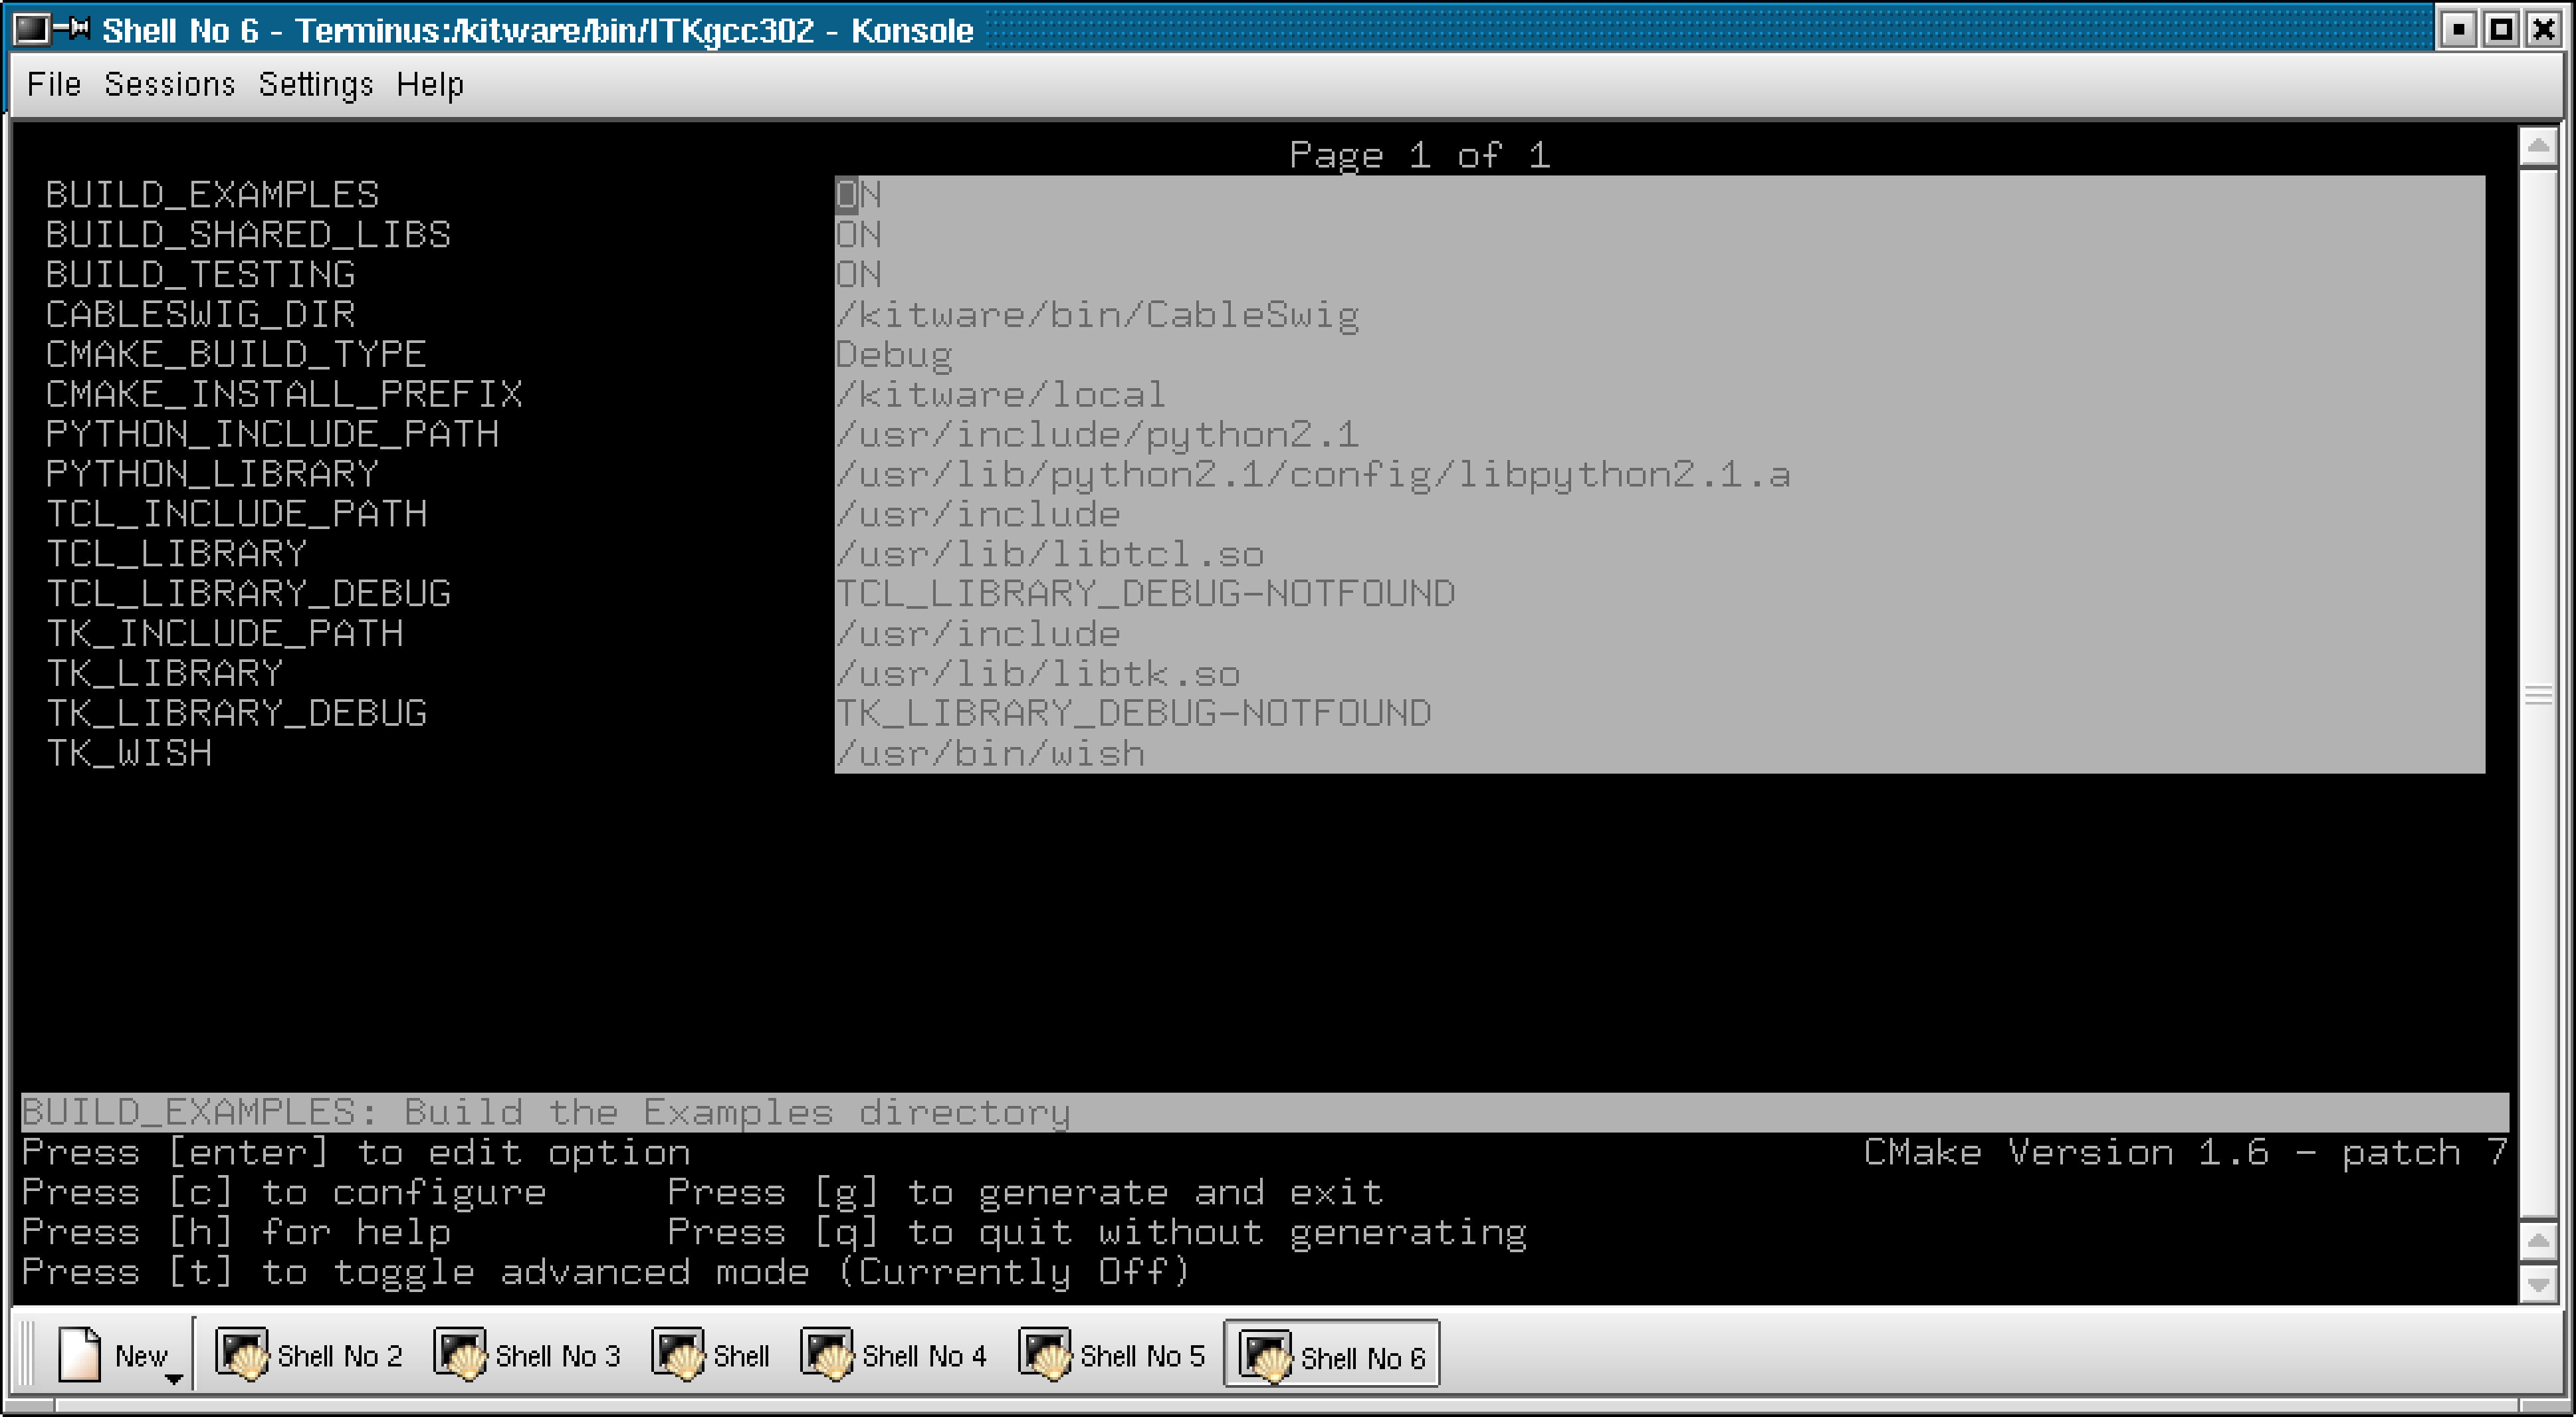
\includegraphics[height=0.45\textwidth]{ccmakeScreenShot.eps}
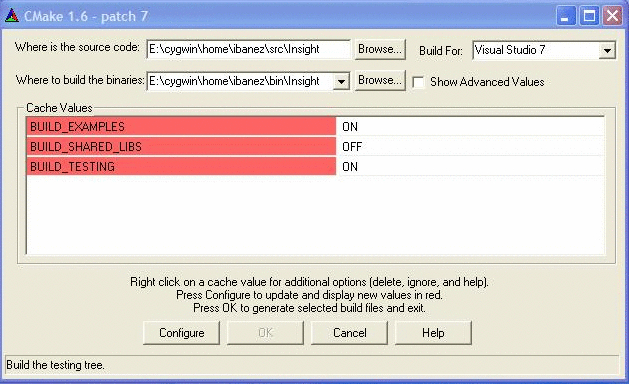
\includegraphics[height=0.45\textwidth]{CMakeSetupScreenShot.eps}
\caption{CMake interface. Left) \texttt{ccmake}, the UNIX version based on
\texttt{curses}. Right) \texttt{CMakeSetup}, the MS-Windows version based on MFC}
\label{fig:CMakeGUI}
\end{figure}

Figure \ref{fig:CMakeGUI} shows the CMake interface for UNIX and MS-Windows.
In order to speed up the build process you may want to disable the
compilation of the demo applications. This is done with the variable
\code{BUILD\_APPLICATIONS=OFF}. The demo applications  distributed with the
toolkit are a helpful resource for learning how to write applications with
ITK.  However, due to the large number of examples and the fact that some of
them rely on third party libraries, enabling this option will considerably
complicate the initial configuration of the toolkit and is to be avoided the
first time.

Begin running CMake by using \code{ccmake} on Unix, and \code{CmakeSetup} on
Windows. Remember to run \code{ccmake} from the build directory on Unix. On
Windows, specify the source and build directories in the GUI. Then begin to
set the build variables in the GUI if necessary.  (Most variables should have
default values that are sensible.) Each time you change a set of variables in
CMake, it is necessary to proceed to another configuration step. In the
Windows version this is done by clicking on the ''Configure'' button. In the
UNIX version this is done in a
\code{curses} interface where you can select to configure by hitting the
''c'' key.

When no new options appear in CMake, you can proceed to generate Makefiles or
Visual Studio projects. This is done in Windows by clicking on the ''Ok''
button.  In the UNIX version this is done by hitting the ''g'' key. After the
generation process CMake will quit silently. To initate the build
process, you can under UNIX simply type \code{make} while under Window you
will have to load the workspace named \code{ITK.dsw} from the directory that
you provide to CMake as Binary directory.

The build process will typically take from 30 minutes to one hour depending
on the performance of your system. As part of the normal built process, about
300 small test programs are compiled. This allows to verify that the basic
components of ITK have been correctly built on your system.

\section{Getting Started With ITK }
\label{sec:GettingStartedWithITK}
 
The simplest way to get started with ITK is to create a new directory
somewhere in your disk and create two files in it. The first one is a
\code{CMakeLists.txt} file that will be used by CMake to generate a Makefile
(if you are using UNIX) or a Visual Studio workspace (if you are using
MS-Windows).  The second file is an actual C++ program that will exercise
some of the multiple classes available in ITK. The details of these files
are described in the following section.

Once both files are in your directory you can run CMake in order to configure
your project. Under UNIX, you can \code{cd} to your newly created directory
and type \code{"ccmake . "}. Note the "." in the command line for indicating
that the \code{CMakeLists.txt} file is in the current directory. The
\code{curses} interface will require you to provide the directory where ITK
was built. This is the same path that you indicated for the
\code{ITK\_BINARY\_DIR} variable at the time of configuring ITK. Under
Windows you can run \code{CMakeSetup} and provide your newly created
directory as being both the source directory and the binary directory for
your new project (i.e., an in-place build. Then CMake will require you to
provide the path to the binary directory where ITK was built. The ITK binary
directory will contain a file named \code{UseITK.cmake} generated during the
configuration process at the time ITK was built.  From this file, CMake will
recover all the information required to configure your new ITK project.

\subsection{Hello World !}
\label{sec:HelloWorldITK}

\index{Hello World|textbf}

Here is the content of the two files to write in your new project. These two
files can be found in the \code{Insight/Examples/Installation} directory. The
\code{CMakeLists.txt} file contains the following lines:

\begin{verbatim}
PROJECT(HelloWorld)

INCLUDE (${CMAKE_ROOT}/Modules/FindITK.cmake)
IF (USE_ITK_FILE)
  INCLUDE(${USE_ITK_FILE})
ENDIF(USE_ITK_FILE)

ADD_EXECUTABLE(HelloWorld HelloWorld.cxx )

TARGET_LINK_LIBRARIES(HelloWorld ITKCommon)
\end{verbatim}

The first line defines the name of your project as it appears in Visual
Studio (it will have no effect under UNIX). The second line loads a CMake
file with a predefined strategy for finding ITK \footnote{Similar files are
provided in CMake for other commonly used libraries, all of them named
\code{Find*.cmake}}. If the strategy for finding ITK fails, CMake will prompt
you for the directory where ITK is installed in your system. In that case you
will write This information in the \code{ITK\_DIR} variable. The line \code{
INCLUDE(\${USE\_ITK\_FILE})} loads the \code{UseITK.cmake} file containing
all the configuration information from ITK. The \code{LINK\_LIBRARIES} line
specify which ITK libraries will be linked against this project. Finally the
line
\code{ADD\_EXECUTABLE} defines as its first argument the name of the executable
that will be produced as result of this project. The following arguments in
the line are the names of the source files to be compiled and linked.

\input HelloWorld.tex

The Image class is explained in detail in section \ref{sec:ImageSection}.

At this point you have successfully installed and compiled ITK, and created
your first simple program. If you have difficulties, please join the
insight-users mailing list (Section \ref{sec:JoinMailList} on page
\pageref{sec:JoinMailList} and pose questions there.

\chapter{System Overview}
\label{chapter:SystemOverview}

The purpose of this chapter is to provide you with an overview of the
\emph{Insight Toolkit} system. We recommend that you read this chapter to
gain an appreciation for the breadth and area of application of ITK.
(Note: this chapter is not yet completed at this time.)

\section{System Organization}
\label{sec:SystemOrganization}

The Insight Toolkit consists of several subsystems. A brief
description of these subsystems follows. Later sections in this chapter---and
in some cases addtional chapters---cover these concepts in more detail. (Note:
in the previous chapter two other modules---\code{InsightDocumentation} and
\code{InsightApplications} were briefly described.)

\begin{description}
	\item[Essential System Concepts.] Like any software system, ITK is
        built around some core design concepts. Some of the more important
        concepts include generic programming, smart pointers for memory
        management, object factories for adaptable object instantiation,
        event management using the command/observer design paradigm, and
        multithreading support.

	\item[Data Representation and Access.]  Two principle classes are
        used to represent data: the Image and Mesh classes. In addition,
        various types of iterators and containers are used to hold and
        traverse the data. Other important but less popular classes are
        also used to represent data such as histograms and BLOX images.

	\item[Numerics] ITK uses VXL's VNL numerics libraries. These are
        easy-to-use C++ wrappers around the Netlib Fortran numerical 
        analysis routines (\url{http://www.netlib.org}).

	\item[Data Processing Pipeline.]  The data representation classes
        (known as \emph{data objects}) are operated on by \emph{filters} that
        in turn may be organized into data flow pipelines. These pipelines
        maintain state and therefore execute only when necessary, support
        multi-threading, and are streaming capable (i.e., can operate on
        pieces of data to minimize the memory footprint).

        \item[IO Framework.] Associated with the data processing pipeline are
        sources, i.e., filters that initiate the pipeline, and mappers,
        filters that terminate the pipeline. A common type of
        sources are readers, used to input data, and writers, used to
        output data from the pipeline. ITK uses a flexible object factory
        mechanism supporting a variety of file formats.

	\item[Registration Framework.] A flexible framework for registration
        supports four different types of registration: image registration,
        multiresolution registration, PDE based registration, and FEM (finite-
        element, i.e., deformable) registration.

	\item[FEM Framework.] ITK includes a subsystem for solving general
        FEM problems, in particular non-rigid registration. The FEM package
        includes mesh definition (nodes and elements), loads, and boundary
        conditions.

	\item[Spatial Objects.] Geometric shapes are represented in ITK using
        the spatial object hierarchy.  These classes are intended to support
        modeling of anatomical structures. Using a common basic interface,
        the spatial objects are capable of representing regions of space in a
        variety of different ways. For example: mesh structures, image masks,
        and implicit equations may be used as the underlying representation
        scheme.  Spatial objects are a natural data structure for
        communicating the results of segmentation methods and for introducing
        anatomical priors in both segmentation and registration methods.

	\item[Level Set Framework.] The level set framework is a set of
        classes for creating filters to solve partial differential equations
        on images using an iterative, finite difference update scheme. The
        level set framework consists of finite difference solvers including a
        sparse level set solver, a generic level set segmentation filter, and
        several specific subclasses including threshold, Canny, and Laplacian
        based methods.

	\item[Wrapping.] ITK uses a unique, powerful system for producing
        interfaces (i.e., ``wrappers'') to interpreted languages such as Tcl
        and Python. The CABLE system is capable of wrapping C++ code of
        arbitrary complexity because it uses a compiler to parse the code.
        The parsed code is in turn represented using XML which is then
        used to build the language interfaces.

	\item[Auxiliary / Utilities] Several auxiliary subsystems are 
        available to supplement other classes in the system. For example,
        calculators are classes that perform specialized operations in
        support of filters (e.g., MeanCalculator computes the mean of a
        sample). Other utilities include a partial DICOM parser, MetaIO file
        support, png, zlib, FLTK / Qt image viewers, and interfaces to the
        Visualization Toolkit (VTK) system.
        
\end{description}


\section{Essential System Concepts}
\label{sec:EssentialSystemConcepts}

This section describes some of the core concepts and implementation features
found in ITK.

\subsection{Generic Programming}
\label{sec:GenericProgramming}

Generic programming is a method of organizing libraries consisting of
generic---or reusable---software components \cite{Musser1996}. The idea is to
make software that is capable of ``plugging together'' in an efficient,
adaptable manner. The essential ideas of generic programming are
\emph{containers} to hold data, \emph{iterators} to access the data, and 
\emph{generic algorithms} that use containers and iterators to create 
efficient, fundamental algorithms such as sorting. Generic programming is
implemented in C++ with the \emph{template} programming mechanism and the 
use of the STL Standard Template Library \cite{Austern1999}.

C++ templating is a programming technique allowing users to write software in
terms of one or more unknown types \code{T}. To create executable code, the
user of the software must specify all types \code{T} (known as \emph{template
instantiation} and successfully process the code with the compiler. The
\code{T} may be a native type such as
\code{float} or \code{int}, or \code{T} may be a user-defined type (e.g.,
\code{class}). At compile-time, the compiler makes sure that the templated 
types are compatible with the instantiated code and that the types are
supported by the necessary functions and operators.

ITK uses the techniques of generic programming in its implementation. The
advantage of this approach is that an almost unlimited variety of data types
are supported simply by defining the appropriate template types. For example,
in ITK it is possible to create images consisting of almost any type of
pixel. In addition, the type resolution is performed at compile-time, so the
compiler can optimize the code to deliver maximal performance. The
disadvantage of generic programming is that many compilers still do not
support these advanced concepts and cannot compile ITK. And even if they do,
they may produce completely undecipherable error messages due to even the
simplest syntax errors. If you are not familiar with templated code and
generic programming, we recommend the two books cited above.

\subsection{Include Files and Class Definitions}
\label{sec:IncludeFiles}

In ITK classes are defined by a maximum of two files: a header \code{.h} file
and an implementation file---\code{.cxx} if a non-templated class, and a
\code{.txx} if a templated class. The header files contains documentation that
is used by the Doxygen documentation systen to produce the HTML manual pages.

In addition to class headers, there are a few other important header files.
\begin{description}
        \item[\code{itkMacro.h}] is found in the \code{Code/Common} directory

        and defines standard system-wide macros (such as \code{Set/Get},
        constants, and other parameters.

        \item[\code{itkNumericTraits.h}] is found in the \code{Code/Common} 
        directory and defines numeric characteristics for native types such
        as its maximum and minimum possible values.

        \item[\code{itkWin32Header.h}] is found in the \code{Code/Common} 
        and is used to define operating system parameters to control
        the compilatilation process.
\end{description}

\subsection{Smart Pointers}
\label{sec:SmartPointers}

By their nature object-oriented systems represent and operate on data through
a variety of object types, or classes. When a particular class is
instantiated to produce an instance of that class, memory allocation occurs
so that the instance can store data attribute values and method pointers
(i.e., the vtable). This object may then be referenced by other classes or
data structures during normal operation of the program. At some
point---certainly by the time the program is exiting---all references to that
instance disappear. At this point, the instance must be deleted to recover
the valuable memory resource that the instance no longer requires. This process
is known as memory management.

In ITK, memory management is implemented through reference counting. This
compares to another popular approach---garbage collection---used by many
systems including Java. In reference counting, a count of the number of
references to each instance is kept. When the reference goes to zero, the
object destroys itself. In garbage collection, a background process sweeps
the system identifying instances no longer referenced in the system and
deletes them. The problem with garbage collection is that the actual point in
time at which memory is deleted is variable. This is unacceptable when an
object size may be gigantic (think of a large 3D volume gigabytes in
size). Reference counting deletes memory immediately.

Reference counting is implemented as follows. Instances have a
\code{Register()} method invoked on them by a class that uses the
instance. The \code{Register()} method increments the instances' reference
count. When the reference to the instance disappears, a \code{Delete()}
method is invoked on the instance---this is equivalent to an
\code{UnRegister()} method that decrements the reference count. When the
reference count returns to zero, the instance is destroyed.

This protocol is greatly simplified by using a helper class called a
\code{SmartPointer}. The smart pointer acts like a regular pointer 
(e.g. supports operators \code{->} and \code{*}) but automagically
performs a \code{Register()} when referring to an instance, and an
\code{UnRegister()} when it no longer points to the instance.  Unlike
most other instances in ITK, \code{SmartPointer}s can be allocated
on the program stack, and are automatically deleted when the scope in
which the \code{SmartPointer} was created is closed. As a result, you should
\emph{rarely if ever call Register() or Delete()} in ITK. For example:

\begin{verbatim}
  MyRegistrationFunction()
    { <----- Start of scope

    // here an interpolator is created and associated to the
    // SmartPointer "interp".
    InterpolatorType::Pointer interp = InterpolatorType::New();

    } <------ End of scope
\end{verbatim}


At the end of scope, the \code{SmartPointer} \code{interp} is destroyed, the
reference count of the actual interpolator object is decremented, and if it
reaches zero, then the interpolator is also destroyed.

%\subsection{Object Factories}
%\label{sec:ObjectFactories}



\subsection{Multi-Threading}
\label{sec:MultiThreading}

Multithreading is handled in ITK in a generic manner. The class
\code{itk::MultiThreader} provides support for multithreaded execution using
\code{sproc()} on an SGI, or \code{pthread\_create} on any platform supporting 
POSIX threads.  This class can be used to execute a single method on multiple
threads, or to specify a method per thread.

%\subsection{Event Handling}
%\label{sec:EventHandling}


%\section{Data Representation and Access}
%\label{sec:DataRepresentationAndAccess}
%
%	mesh, image, iterators, various containers
%
\section{Numerics}
\label{sec:Numerics}

ITK uses the \code{VNL} numerics library and provides extra functionality
beyond \code{VNL} including interface classes to ITK proper.  The numerics
library, \code{VNL} is intended to provide an environment for numerical
programming which combines the ease of use of packages like Mathematica and
Matlab with the speed of C and the elegance of C++. It provides a C++
interface to the high-quality Fortran routines made available in the public
domain by numerical analysis researchers.

The VNL numerics library includes classes for 
\begin{description}
        \item[Matrices and vectors.] Standard matrix and vector support
        and operations on these types.

        \item[Specialized matrix and vector classes.] Several special matrix
        and vector class with special numerical properties are
        available. Class \code{vnl\_diagonal\_matrix} provides a fast and
        convenient diagonal matrix, while fixed size matrices and vectors
        allow "fast-as-C" computations (see \code{vnl\_matrix\_fixed<T,n,m>} 
        and example subclasses \code{vnl\_double\_3x3} and 
        \code{vnl\_double\_3}).

        \item[Matrix decompositions.] Classes \code{vnl\_svd<T>}, 
        \code{vnl\_symmetric\_eigensystem<T>}, and 
        \code{vnl\_generalized\_eigensystem}. 

        \item[Real polynomials.] Class \code{vnl\_real\_polynomial} stores 
        the coefficients of a real polynomial, and provides methods of 
        evaluation of the polynomial at any x, while class 
        \code{vnl\_rpoly\_roots} provides a root finder. 

        \item[Optimization.] Classes \code{vnl\_levenberg\_marquardt},
        \code{vnl\_amoeba}, \code{vnl\_lbfgs},
        \code{vnl\_conjugate\_gradient} allow optimization of user-supplied
        functions either with or without user-supplied derivatives.

        \item[Standardized functions and constants.] Class \code{vnl\_math}
        defines constants (pi, e, eps...) and simple functions (sqr, abs,
        rnd...). Class \code{numeric\_limits} is from the ISO standard
        document, and provides a way to access basic limits of a
        type. E.g. \code{numeric\_limits<short>::max()} returns the maximum
        value of a short.
\end{description}

Most VNL routines are implemented as wrappers around the high-quality Fortran
routines which have been developed by the numerical analysis community over
the last forty years and placed in the public domain. The central repository
for these programs is the "netlib" server \url{http://www.netlib.org/}. The
National Institute of Standards and Technology (NIST) provides an excellent
search interface to this repository in its Guide to Available Mathematical
Software (GAMS) at \url{http://gams.nist.gov}, both as a decision tree and a
text search.

ITK provides additional numerics functionality. A suite of optimizers, that
use \code{VNL} under the hood and integrate with the registration framework
are available. A large collection of statistics functions---not available from
\code{VNL}---are also provided in the \code{Insight/Numerics/Statistics}
directory. In addition, a complete finite element (FEM) package is available,
primarily to support the deformable registration in ITK.

%\section{Data Processing Pipeline}
%\label{sec:DataProcessingPipeline}
%
%filters, mappers, update
%
%\section{Registration Framework}
%\label{sec:RegistrationFramework}
%
%blah blah
%
%\section{FEM Framework}
%\label{sec:FEMFramework}
%
%blah blah
%
\section{Spatial Objects}
\label{sec:SpatialObjects}
%
The ITK spatial object framework supports the philosophy that the task of
image segmentation and registration is actually the task of object
processing. The image is but one medium for representing objects of interest,
and much processing and data analysis can and should occur at the object
level and not based on the medium used to represent the object.

ITK spatial objects provide a common interface for accessing the physical
location and geometric properties of and the relationship between objects in
a scene that is independent of the form used to represent those objects. That
is, the internal representation maintained by a spatial object may be a list
of points internal to an object, the surface mesh of the object, a continuous
or parametric representation of the object's internal points or surfaces, and
so forth.

The capabilities provided by the spatial objects framework supports their use
in object segmentation, registration, surface/volume rendering, and other
display and analysis functions. The spatial object framework extends the
concept of a "scene graph" that is common to computer rendering packages so
as to support these new functions. With the spatial objects framework you
can:
\begin{enumerate}

        \item Specify a spatial object's parent and children objects.  In
        this way, a liver may contain vessels and those vessels can be
        organized in a tree structure.

        \item Query if a physical point is inside of an object or
        (optionally) any of its children.

        \item Request the value and derivatives at a physical point as
        specified by an object or (optionally) its children.

        \item Specify the coordinate transformation that maps a parent
        object's coordinate system into a child object's coordinate system.

        \item Compute the bounding box of a spatial object and (optionally)
        its children.

        \item Query the resolution at which the object was originally
        computed.  For example, you can query the resolution (i.e., voxel
        spacing) of the image used to generate a particular instance of a
        \code{BlobSpatialObject}.
\end{enumerate}

Currently implemented types of spatial objects include: Blob, Ellipse, Group,
Image, Line, Surface, and Tube.  The \code{itk::Scene} object is used to hold
a list of spatial objects that may in-turn have children.  Each spatial
object can be assigned a color property.  Each spatial object type has its
own capabilities. For example, \code{TubeSpatialObject}s indicate to what
point on their parent tube they connect.

There are a limited number of spatial objects and their methods in ITK, but
their number is growing and their potential is huge. Using the nominal
spatial object capabilities methods, such as marching cubes or mutual
information registration, can be applied to objects regardless of their
internal representation. By having a common API, the same method can be used
to register a parametric representation of a heart with an individual's CT
data or to register two hand segmentations of a liver.

%blah blah
%
%\section{Level Set Framework}
%\label{sec:LevelSetFramework}
%
%blah blah
%
%\section{Wrapping}
%\label{sec:Wrapping}
%
%blah blah
%
%\section{Auxiliary \& Utilities}
%\label{sec:Auxiliary}
%\label{sec:Utilities}
%
%calculators and classes supporting the data processing pipeline;
%utilities such as GUI interface tools

\fi


\part{User's Guide}

\ifitkFullVersion

\chapter{DataRepresentation}
\label{sec:DataRepresentation}


This chapter introduces the basic classes responsible
for carrying data in ITK. The most common classes are the
\code{itk::Image},  the \code{itk::Mesh} and the \code{itk::PointSet}.

\section{Image}
\label{sec:ImageSection}

The Image class follows the spirit of Generic Programming where
types are separated from the algorithmic behavior of the class.
ITK supports images with any pixel type and any spatial dimension.

\subsection{Creating an Image}\label{sec:CreatingAnImageSection}


\input Image1.tex

In practice it is rare to allocate and initialize an image directly.
Typically the image is read from a source like a file or a data acquisition
card. The following example illustrates how an image can be read from
a file.




\subsection{Reading an Image from a file}
\label{sec:ReadingImageFromFile}

\input Image2.tex





\subsection{Accessing pixel data}
\label{sec:AccessingImagePixelData}

\input Image3.tex




\subsection{Defining Origin and Spacing}
\label{sec:DefiningImageOriginAndSpacing}

\input Image4.tex


\subsection{RGB Images}
\label{sec:DefiningRGBImages}

\input RGBImage.tex


\subsection{Vector Images}
\label{sec:DefiningVectorImages}

\input VectorImage.tex



\section{PointSet}
\label{PointSetSection}

\subsection{Creating a PointSet}
\label{sec:CreatingAPointSet}

\input PointSet1.tex



\subsection{Getting access to points}
\label{sec:GettingAccessToPointsInThePointSet}

\input PointSet2.tex



\subsection{Getting access to data in points}
\label{sec:GettingAccessToDataInThePointSet}

\input PointSet3.tex



\subsection{RGB as pixel type}
\label{sec:PointSetWithRGBAsPixelType}

\input RGBPointSet.tex




\subsection{Vectors as pixelType}
\label{sec:PointSetWithVectorsAsPixelType}

\input PointSetWithVectors.tex



\subsection{Normals as pixelType}
\label{sec:PointSetWithCovariantVectorsAsPixelType}

\input PointSetWithCovariantVectors.tex




\section{Mesh}\label{MeshSection}

\subsection{Creating a Mesh}
\label{sec:CreatingAMesh}

\input Mesh1.tex


\subsection{Inserting Cells}
\label{sec:InsertingCellsInMesh}

\input Mesh2.tex


\subsection{Managing Data in Cells}
\label{sec:ManagingCellDataInMesh}

\input Mesh3.tex


\subsection{Customizing the Mesh}
\label{sec:CustomizingTheMesh}

\input MeshTraits.tex


\subsection{Topology and the K-Complex}
\label{sec:MeshKComplex}

\input MeshKComplex.tex


\subsection{Iterating Throught Cells}
\label{sec:MeshCellsIteration}

\input MeshCellsIteration.tex


\subsection{Visiting Cells}
\label{sec:MeshCellVisitor}

\input MeshCellVisitor.tex


\subsection{More on Visiting Cells}
\label{sec:MeshCellVisitorMultipleType}

\input MeshCellVisitor2.tex



\fi

\ifitkFullVersion
\chapter{Filtering}

This chapter introduces the most commonly used filters in the toolkit.  Most of
these filters are intended to process images. They will accept one or more
images as input and will produce one or more images as output. Insight is based
on a data pipeline architecture in which the output of one filter is passed as
input to another filter.


\section{Thresholding}
\ifitkFullVersion
\label{sec:ThresholdingFiltering}
\fi

\subsection{Binary Thresholding}
\label{sec:BinaryThresholdingImageFilter}

\ifitkFullVersion
\input{BinaryThresholdImageFilter.tex}
\fi

\subsection{Thresholding}
\label{sec:ThresholdingImageFilter}

\ifitkFullVersion
\input{ThresholdImageFilter.tex}
\fi



\section{Casting}
\label{sec:CastingImageFilters}

The filters discussed in this section perform pixel-wise intensity mappings.
This is usually desired as a parallel action to image pixel-type casting since
the input and output pixel-types have in general different dynamic ranges.

\subsection{Linear Mappings}
\label{sec:IntensityLinearMapping}

%\ifitkFullVersion
\input{CastingImageFilters.tex}
%\fi

\subsection{Non Linear Mappings}
\label{sec:IntensityNonLinearMapping}

The following filter can be seen as a variant of the casting filters. Its main
difference is the use of a smooth and continuous transtion function of
non-linear form.

%\ifitkFullVersion
\input{SigmoidImageFilter.tex}
%\fi
  

\section{Gradients}
\label{sec:GradientFiltering}

Computation of gradients is a fairly common operation in image processing. The
term is sometimes loosely used to refer the gradient vectors or the magnitude
of this gradient. Insight filters attempt to reduce this ambiguity by including
the \emph{magnitude} term when appropriate. Insight provides filters for
computing both the image of gradient vectors and the image of magnitudes.

\subsection{Gradient Magnitude}
\label{sec:GradientMagnitudeImageFilter}

\ifitkFullVersion
\input{GradientMagnitudeImageFilter.tex}
\fi

\subsection{Gradient Magnitude With Smoothing}
\label{sec:GradientMagnitudeRecursiveGaussianImageFilter}

\ifitkFullVersion
\input{GradientMagnitudeRecursiveGaussianImageFilter.tex}
\fi




\section{Neighborhood Filters}
\label{sec:NeighborhoodFilters}

The concept locality is frequently encountered in image processing on the form
of filters that compute every output pixel using information from a reduced
region on the neighborhood of the input pixel. The classical form of this
filters are the $3 \times 3$ filters in 2D images. Convolution masks based on
these neighborhoods could perform diverse tasks ranging from noise reduction,
to differential operations, to mathematical morphology.

The Insight toolkit implements an elegant approach for the computation of these
family of filters. The input image is visited by a special iterator called the
\code{NeighborhoodIterator}. This iterator is capable of moving over all
the pixels in an image and for each position it can address the pixels in a
local neighborhood. Operators can be defined in order to specify what
algorithmic operation must be performed on the neighborhood of the input pixel
to compute the value of the output pixel. The following section describes some
of the commonly used filters that take advantage of this construction.  

\subsection{Mean Filter}
\label{sec:MeanFilter}

\ifitkFullVersion
\input{MeanImageFilter.tex}
\fi

\subsection{Median Filter}
\label{sec:MedianFilter}

\ifitkFullVersion
\input{MedianImageFilter.tex}
\fi


\subsection{Mathematical Morphology}
\label{sec:MathematicalMorphology}

Mathematical morphology has proved to be a a powerful resource for image
processing and analysis \cite{Serra1982}. Insight implements mathematical
morphology filters using the approach of \code{NeighborhoodIterator}s and
\code{NeighborhoodOperator}s. Two basic flavors of filters are available in the
toolkit, the ones that operate on binary images and the ones that operate on
grayscale images. 

\subsubsection{Binary Filters}
\label{sec:MathematicalMorphologyBinaryFilters}

\ifitkFullVersion
\input{MathematicalMorphologyBinaryFilters.tex}
\fi


\subsubsection{Grayscale Filters}
\label{sec:MathematicalMorphologyGrayscaleFilters}

\ifitkFullVersion
\input{MathematicalMorphologyGrayscaleFilters.tex}
\fi




\section{Smoothing Filters}
\label{sec:SmoothingFilters}

Real image data has a level of uncertainty that is manifested on the
variability of measures assigned to pixels. This is usually interpreted as
noise and considered an undesirable component of the image data. This section
describes several methods that can be applied to reduce noise on images.

\subsection{Blurring}
\label{sec:BlurringFilters}

Blurring is the traditional approach for removing noise from images. It it
usually implemented in the form of a convolution with a kernel. The effect of
this operation on the image spectrum is to attenuate high spatial frequencies.
Different kernels attenuate frequencies in different ways. One of the most
commonly used kernels is the Gaussian. Two implementations of Gaussian
smoothing are available in the toolkit. The first one is based on a traditional
convolution while the other is based on the application of IIR filters that
approximate the convolution with a Gaussian \cite{Deriche1990,Deriche1993}. 

\subsubsection{Discrete Gaussian}
\label{sec:DiscreteGaussianImageFilter}

\ifitkFullVersion
\input{DiscreteGaussianImageFilter.tex}
\fi


\subsubsection{Binomial Blurring}
\label{sec:BinomialBlurImageFilter}

\ifitkFullVersion
\input{BinomialBlurImageFilter.tex}
\fi

\subsubsection{Recursive Gaussian IIR}
\label{sec:RecursiveGaussianImageFilter}

\ifitkFullVersion
\input{SmoothingRecursiveGaussianImageFilter.tex}
\fi



\subsection{Edge Preserving Smoothing}
\label{sec:EdgePreservingSmoothingFilters}

\subsubsection{Introduction to Anisotropic Diffusion}
\label{sec:IntroductionAnisotropicDiffusion}
\ifitkFullVersion
%
%
%  This file in inserted in the Filtering.tex file.
%
%

The drawback of image denoising (smoothing) is that it tends to blur away the
sharp boundaries in the image that help to distinguish between the
larger-scale anatomical structures that one is trying to characterize (which
also limits the size of the smoothing kernels in most applications).  Even in
cases where smoothing does not obliterate boundaries, it tends to distort the
fine structure of the image and thereby changes subtle aspects of the
anatomical shapes in question.

Perona and Malik \cite{Perona1990} introduced an alternative to
linear-filtering that they called \emph{anisotropic diffusion}.  Anisotropic
diffusion is closely related to the earlier work of Grossberg
\cite{Grossberg1984}, who used similar nonlinear diffusion processes to model
human vision.  The motivation for anisotropic diffusion (also called
\emph{nonuniform} or \emph{variable conductance} diffusion) is that a Gaussian
smoothed image is a single time slice of the solution to the heat equation,
that has the original image as its initial conditions.  Thus, the solution to
\begin{equation} \frac{\partial g(x, y, t) }{\partial t} = \nabla \cdot \nabla
g(x, y, t), \end{equation} where $g(x, y, 0) = f(x, y)$ is the input image, is
$g(x, y, t) = G(\sqrt{2t}) \otimes f(x, y)$, where $G(\sigma)$ is a Gaussian
with standard deviation $\sigma$.

Anisotropic diffusion includes a variable conductance term that, in turn,
depends on the differential structure of the image.  Thus, the variable
conductance can be formulated to limit the smoothing at ``edges'' in images, as
measured by high gradient magnitude, for example. \begin{equation} g_{t} = \nabla \cdot
c(\left| \nabla g \right|) \nabla g, \label{eq:aniso} \end{equation} where, for
notational convenience, we leave off the independent parameters of $g$ and use
the subscripts with respect to those parameters to indicate partial
derivatives.  The function $c(|\nabla g|)$ is a fuzzy cutoff that reduces the
conductance at areas of large $|\nabla g|$, and can be any one of a number of
functions.  The literature has shown \begin{equation} c(|\nabla g|) =
e^{-\frac{|\nabla g|^{2}}{2k^{2}}} \end{equation} to be quite effective.
Notice that conductance term introduces a free parameter $k$, the {\em
conductance parameter}, that controls the sensitivity of the process to edge
contrast.  Thus, anisotropic diffusion entails two free parameters: the
conductance parameter, $k$, and the time parameter, $t$, that is analogous to
$\sigma$, the effective width of the filter when using Gaussian kernels.

Equation \ref{eq:aniso} is a nonlinear partial differential equation that can
be solved on a discrete grid using finite forward differences.  Thus, the
smoothed image is obtained only by an iterative process, not a convolution or
non-stationary, linear filter.  Typically, the number of iterations required
for practical results are small, and large 2D images can be processed in
several tens of seconds using carefully written code running on modern, general
purpose, single-processor computers.  The technique applies readily and
effectively to 3D images, but requires more processing time.

In the early 1990's several research groups \cite{Gerig1991,Whitaker1993d}
demonstrated the effectiveness of anisotropic diffusion on medical images.  In
a series of papers on the subject
\cite{Whitaker1993,Whitaker1993b,Whitaker1993c,Whitaker1993d,Whitaker-thesis,Whitaker1994},
Whitaker described a detailed analytical and empirical analysis, introduced a
smoothing term in the conductance that made the process more robust, invented a
numerical scheme that virtually eliminated directional artifacts in the
original algorithm, and generalized anisotropic diffusion to vector-valued
images, an image processing technique that can be used on vector-valued medical
data (such as the color cryosection data of the Visible Human Project).

For a vector-valued input $\vec{F}:U \mapsto \Re^{m}$ the process takes the
form \begin{equation} \vec{F}_{t} = \nabla \cdot c({\cal D}\vec{F}) \vec{F},
\label{eq:vector_diff} \end{equation} where ${\cal D}\vec{F}$ is a {\em
dissimilarity} measure of $\vec{F}$, a generalization of the gradient magnitude
to vector-valued images, that can incorporate linear and nonlinear coordinate
transformations on the range of $\vec{F}$.  In this way, the smoothing of the
multiple images associated with vector-valued data is coupled through the
conductance term, that fuses the information in the different images.  Thus
vector-valued, nonlinear diffusion can combine low-level image features (e.g.
edges) across all ``channels'' of a vector-valued image in order to preserve or
enhance those features in all of image ``channels''.

Vector-valued anisotropic diffusion is useful for denoising data from devices
that produce multiple values such as MRI or color photography.  When performing
nonlinear diffusion on a color image, the color channels are diffused
separately, but linked through the conductance term. Vector-valued diffusion
is also useful for processing registered data from different devices or for
denoising higher-order geometric or statistical features from scalar-valued
images \cite{Whitaker1994,Yoo1993}.

The output of anisotropic diffusion is an image or set of images that
demonstrates reduced noise and texture but preserves, and can also enhance,
edges.  Such images are useful for a variety of  processes including
statistical classification, visualization, and geometric feature extraction.
Previous work has shown \cite{Whitaker-thesis} that anisotropic diffusion, over
a wide range of conductance parameters, offers quantifiable advantages over
linear filtering for edge detection in medical images.

Since the effectiveness of nonlinear diffusion was first demonstrated, numerous
variations of this approach have surfaced in the literature \cite{Romeny1994}.
These include alternatives for constructing dissimilarity measures
\cite{Sapiro1996}, directional (i.e., tensor-valued) conductance terms
\cite{Weickert1996,Alvarez1994} and level set interpretations
\cite{Whitaker2001}.

\fi


\subsubsection{Curvature Flow}
\label{sec:CurvatureFlowImageFilter}

\ifitkFullVersion
\input{CurvatureFlowImageFilter.tex}
\fi


\subsubsection{MinMaxCurvature Flow}
\label{sec:MinMaxCurvatureFlowImageFilter}

\ifitkFullVersion
\input{MinMaxCurvatureFlowImageFilter.tex}
\fi



\subsubsection{BinaryMinMaxCurvature Flow}
\label{sec:BinaryMinMaxCurvatureFlowImageFilter}

\ifitkFullVersion
\input{BinaryMinMaxCurvatureFlowImageFilter.tex}
\fi


\subsubsection{Gradient Anisotropic Diffusion}
\label{sec:GradientAnisotropicDiffusionImageFilter}

\ifitkFullVersion
\input{GradientAnisotropicDiffusionImageFilter.tex}
\fi



\subsubsection{Curvature Anisotropic Diffusion}
\label{sec:CurvatureAnisotropicDiffusionImageFilter}

\ifitkFullVersion
\input{CurvatureAnisotropicDiffusionImageFilter.tex}
\fi


\subsubsection{Bilateral Filter}
\label{sec:BilateralImageFilter}

\ifitkFullVersion
\input{BilateralImageFilter.tex}
\fi



\subsection{Edge Preserving Smoothing in Vector Images}
\label{sec:VectorAnisotropicDiffusion}

Anisotropic diffusion can also be applied to images whose pixels are vectors.
In this case the diffusion is computed independently for each vector component.
The following classes implement versions of anisotropic diffusion on vector images.


\subsubsection{Vector Gradient Anisotropic Diffusion}
\label{sec:VectorGradientAnisotropicDiffusionImageFilter}

\ifitkFullVersion
\input{VectorGradientAnisotropicDiffusionImageFilter.tex}
\fi

\subsubsection{Vector Curvature Anisotropic Diffusion}
\label{sec:VectorCurvatureAnisotropicDiffusionImageFilter}

\ifitkFullVersion
\input{VectorCurvatureAnisotropicDiffusionImageFilter.tex}
\fi



\subsection{Edge Preserving Smoothing in Color Images}
\label{sec:ColorAnisotropicDiffusion}

\subsubsection{Gradient Anisotropic Diffusion}
\label{sec:ColorGradientAnisotropicDiffusion}

\ifitkFullVersion
\input{RGBGradientAnisotropicDiffusionImageFilter.tex}
\fi

\subsubsection{Curvature Anisotropic Diffusion}
\label{sec:ColorCurvatureAnisotropicDiffusion}

\ifitkFullVersion
\input{RGBCurvatureAnisotropicDiffusionImageFilter.tex}
\fi



\section{Distance Map}
\label{sec:DistanceMap}

\ifitkFullVersion
\input{DanielssonDistanceMapImageFilter.tex}
\fi



\section{Geometrical Transformations}
\label{sec:GeometricalTransformationFilters}

\subsection{Resample Image Filter}
\label{sec:ResampleImageFilter}

\subsubsection{Introduction}

\ifitkFullVersion
\input{ResampleImageFilter.tex}
\fi

\subsubsection{Importance of Spacing and Origin}
\ifitkFullVersion
\input{ResampleImageFilter2.tex}
\fi

\subsubsection{A full example}
\ifitkFullVersion
\input{ResampleImageFilter3.tex}
\fi

\subsubsection{Rotating an Image}
\ifitkFullVersion
\input{ResampleImageFilter4.tex}
\fi

\subsubsection{Rotating and Scaling an Image}
\ifitkFullVersion
\input{ResampleImageFilter5.tex}
\fi



\fi

\ifitkFullVersion


\chapter{Reading and Writing Images}
\label{sec:IO}

This chapter describes the toolkit architecture supporting reading and
writing of images to files. ITK does not enforce any particular file format,
instead, it provides a structure supporting a variety of formats that can
be easily extended by the user as new formats become available.

We begin the chapter with some simple examples of file I/O.

\section{Basic Example}
\label{sec:ImagReadWrite}
\input{ImageReadWrite.tex}

To better understand the IO architecture, please refer to Figures 
\ref{fig:ImageIOCollaborationDiagram}, 
\ref{fig:ImageIOFactoriesUseCases}, and
\ref{fig:ImageIOFactoriesClassDiagram}. 

\begin{figure}
\center
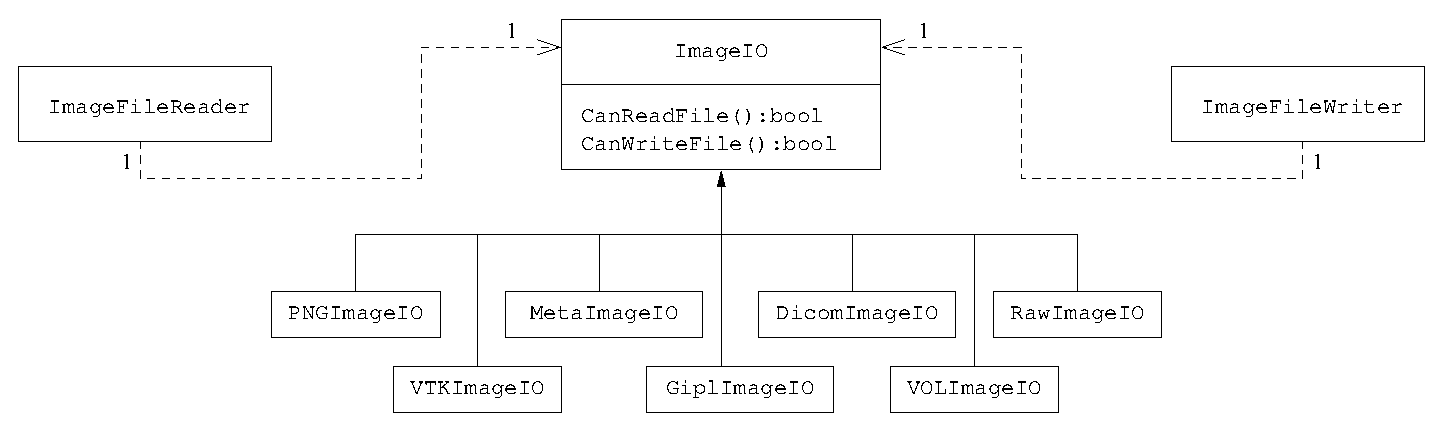
\includegraphics[width=\textwidth]{ImageIOCollaborationDiagram.eps}
\itkcaption[Collaboration diagram of the ImageIO classes]{Collaboration diagram
of the ImageIO classes.} \label{fig:ImageIOCollaborationDiagram}
\end{figure}

\begin{figure}
\center
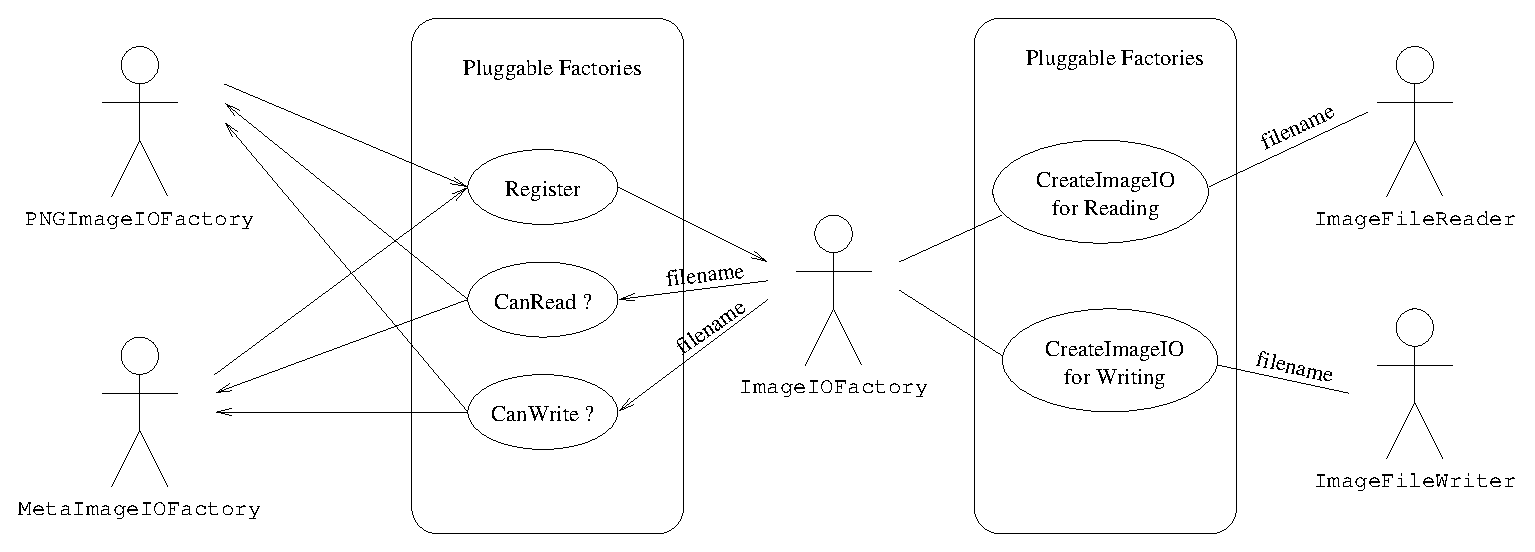
\includegraphics[width=\textwidth]{ImageIOFactoriesUseCases.eps}
\itkcaption[Use cases of ImageIO factories] {Use cases of ImageIO factories.}
\label{fig:ImageIOFactoriesUseCases}
\end{figure}

\begin{figure}
\center
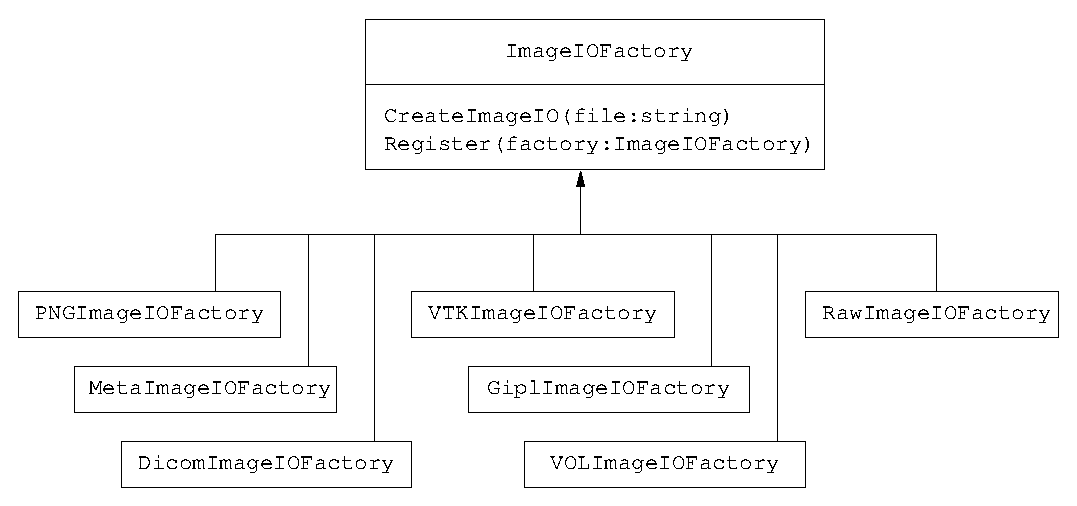
\includegraphics[width=\textwidth]{ImageIOFactoriesClassDiagram.eps}
\itkcaption[Class diagram of ImageIO factories] {Class diagram of the ImageIO
factories.}
\label{fig:ImageIOFactoriesClassDiagram}
\end{figure}

\section{Reading and Writing RGB Images}
\label{sec:RGBImagReadWrite}
\input{RGBImageReadWrite.tex}

\section{Reading, Casting and Writing Images}
\label{sec:ImagReadCastWrite}
\input{ImageReadCastWrite.tex}

\section{Extracting Regions}
\label{sec:ImagReadRegionOfInterestWrite}
\input{ImageReadRegionOfInterestWrite.tex}

\section{Extracting Slices}
\label{sec:ImagReadExtractWrite}
\input{ImageReadExtractWrite.tex}


\section{Reading and Writing Vector Images}
\label{sec:VectorImagReadWrite}

Images whose pixel type is a Vector, a CovariantVector, an Array, or a Complex
are quite common in image processing. It is convenient then to describe rapidly
how those images can be saved into files and how they can be read from those
files later on.

\subsection{The Minimal Example}
\label{VectorImageReadWrite}
\input{VectorImageReadWrite.tex}

\subsection{Producing and Writing Covariant Images}
\label{CovariantVectorImageWrite}
\input{CovariantVectorImageWrite.tex}

\subsection{Reading Covariant Images}
\label{CovariantVectorImageRead}
Let's now take the image that we just created and read it into another program.
\input{CovariantVectorImageRead.tex}


\section{Reading and Writing Complex Images}
\label{sec:ComplexImagReadWrite}
\input{ComplexImageReadWrite.tex}


\section{Extracting Components from Vector Images}
\label{sec:VectorImageExtractComponent}
\input{CovariantVectorImageExtractComponent.tex}


\section{Reading and Writing Image Series}

It is still quite common to store 3D medical images in sets of files each one
containing a single slice of a volume dataset. Those 2D files can be read as
individual 2D images, or can be grouped together in order to reconstruct a 3D
dataset. The same practice can be extended to higher dimensions, for example,
for managing 4D datasets by using sets of files each one containing a 3D image.
This practice is common in the domain of cardiac imaging, perfusion, functional
MRI and PET. This section illustrates the functionalities available in ITK for
dealing with reading and writing series of images.

\index{Series!Reading}
\index{Series!Writing}
\index{Image Series!Reading}
\index{Image Series!Writing}

\subsection{Reading Image Series}
\label{sec:ReadingImageSeries}
\input{ImageSeriesReadWrite.tex}

\subsection{Writing Image Series}
\label{sec:WritingImageSeries}
\input{ImageReadImageSeriesWrite.tex}

\subsection{Reading and Writing Series of RGB Images}
\label{sec:ReadingWritingRGBImageSeries}
\input{RGBImageSeriesReadWrite.tex}


\section{Reading and Writing DICOM Images}
\label{sec:ReadingDicomImageSeries2}

% Small intro to DICOM file format
\index{DICOM}
\index{DICOM!Standard}
\index{DICOM!Series}
\index{DICOM!Introduction}

\subsection{Foreword}
With the introduction of computed tomography (CT) followed by other digital
diagnostic imaging modalities such as MRI in the 1970's, and the increasing use
of computers in clinical applications, the American College of Radiology
(ACR)\footnote{\url{http://www.acr.org}} and the National Electrical
Manufacturers Association (NEMA)\footnote{\url{http://www.nema.org}} recognized
the need for a standard method for transferring images as well as associated
information between devices manufactured from various vendors.

ACR and NEMA formed a joint committee to develop a standard for Digital Imaging
and COmmunications in Medicine (DICOM).  This standard was developed in liaison
with other Standardization Organizations such as CEN TC251, JIRA including
IEEE, HL7 and ANSI USA as reviewers.

DICOM is a comprehensive set of standards for handling, storing and
transmitting information in medical imaging. The DICOM standard was developed
based on the previous NEMA specification.  The standard specifies a file format
definition as well as a network communication protocol. DICOM was developed to
enable integration of scanners, servers, workstations and network hardware from
multiple vendors into an image archiving and communication system.

DICOM files consist of a header and a body of image data. The header contains
standardized as well as free-form fields. The set of standardized fields is
called the public DICOM dictionary, an instance of this dictionary is available
in ITK in the file~\code{Insight/Utilities/gdcm/Dict/dicomV3.dic}.  The list of
free-form fields is also called the \emph{shadow dictionary}.

A single DICOM file can contain multiples frames, allowing storage of volumes
or animations. Image data can be compressed using a large variety of standards,
including JPEG (both lossy and lossless), LZW (Lempel Ziv Welch), and RLE
(Run-length encoding).

The DICOM Standard is an evolving standard and it is maintained in accordance
with the Procedures of the DICOM Standards Committee. Proposals for
enhancements are forthcoming from the DICOM Committee member organizations
based on input from users of the Standard. These proposals are considered for
inclusion in future editions of the Standard. A requirement in updating the
Standard is to maintain effective compatibility with previous editions.

For a more detailed description of the DICOM standard see~\cite{DICOMStandard}.

The following sections illustrate how to use the functionalities that ITK
provides for reading and writing DICOM files. This is extremely important in
the domain of medical imaging since most of the images that are acquired a
clinical setting are stored and transported using the DICOM standard.

DICOM functionalities in ITK are provided by the GDCM library. This open source
library was developed by the CREATIS
Team~\footnote{http://www.www.creatis.insa-lyon.fr} at
INSA-Lyon~\cite{CreatisINSA-Lyon}.  Although originally this library was
distributed under a LGPL
License\footnote{http://www.gnu.org/copyleft/lesser.html}, the CREATIS Team was
lucid enough to understand the limitations of that license and agreed to adopt
the more open BSD-like
License\footnote{http://www.opensource.org/licenses/bsd-license.php} that is
used by ITK. This change in their licensing made possible to distribute GDCM
along with ITK.

GDCM is still being maintained and improved at the original CREATIS site and
the version distributed with ITK gets updated with major releases of the GDCM
library.

\subsection{Reading and writing a 2D image}
\label{DicomImageReadWrite}
\input{DicomImageReadWrite.tex}

\subsection{Reading a 2D DICOM Serie and writting a volume}
\label{DicomSeriesReadImageWrite2}
\input{DicomSeriesReadImageWrite2.tex}

\subsection{Reading a 2D DICOM serie and writting a 2D DICOM serie}
\label{DicomSeriesReadSeriesWrite}
\input{DicomSeriesReadSeriesWrite.tex}

\subsection{Printing out DICOM tags from one slice}
\label{DicomSeriesReadPrintTags}
\input{DicomSeriesReadPrintTags.tex}

\subsection{Printing out DICOM tags from a serie}
\label{DicomImageReadPrintTags}
\input{DicomImageReadPrintTags.tex}

\subsection{Changing a DICOM header}
\label{DicomImageReadChangeHeaderWrite}
\input{DicomImageReadChangeHeaderWrite.tex}



The following section describes the internals of the IO architecture provided
in the toolkit.

\section{Pluggable Factories}
\label{sec:ImageIOPluggableFactories}

The principle behind the input/output mechanism used in ITK is known as
\emph{pluggable-factories} \cite{Gamma1995}. This concept is illustrated in
the UML diagram in Figure~\ref{fig:ImageIOCollaborationDiagram}. From the
user's point of view the objects responsible for reading and writing files
are the \doxygen{ImageFileReader} and \doxygen{ImageFileWriter}
classes. These two classes, however, are not aware of the details involved in
reading or writing particular file formats like PNG or DICOM.  What they do
is to dispatch the user's requests to a set of specific classes that are
aware of the details of image file formats. These classes are the
\doxygen{ImageIO} classes. The ITK delegation mechanism enables users to
extend the number of supported file formats by just adding new classes to the
ImageIO hierarchy.

Each instance of ImageFileReader and ImageFileWriter has
a pointer to an ImageIO object. If this pointer is empty, it will
be impossible to read or write an image and the image file reader/writer must
determine which ImageIO class to use to perform IO operations.
This is done basically by passing the filename to a centralized class, the
\doxygen{ImageIOFactory} and asking it to identify any subclass of
ImageIO capable of reading or writing the user-specified file. This
is illustrated by the use cases on the right side of
Figure~\ref{fig:ImageIOFactoriesUseCases}.

Each class derived from ImageIO must provide an associated factory
class capable of producing an instance of the ImageIO class. For
example, for PNG files, there is a \doxygen{PNGImageIO} object that knows how
to read this image files and there is a \doxygen{PNGImageIOFactory} class
capable of constructing a PNGImageIO object and returning a pointer
to it.  Each time a new file format is added (i.e., a new ImageIO
subclass is created), a factory must be implemented as a derived class of the
ImageIOFactory class as illustrated in
Figure~\ref{fig:ImageIOFactoriesClassDiagram}.

For example, in order to read PNG files, a PNGImageIOFactory is
created and registered with the central ImageIOFactory
singleton\footnote{\emph{Singleton} means that there is only one instance of
this class in a particular application} class as illustrated in the left side
of Figure~\ref{fig:ImageIOFactoriesUseCases}. When the ImageFileReader asks
the ImageIOFactory for an ImageIO capable of reading the
file identified with \emph{filename} the ImageIOFactory will iterate over the
list of registered factories and will ask each one of them is they know how
to read the file. The factory that responds affirmatively will be used to
create the specific ImageIO instance that will be returned to the
ImageFileReader and used to perform the read operations.

In most cases the mechanism is transparent to the user who onlt interacts
with the ImageFileReader and ImageFileWriter. It is
possible, however, to explicitly select the type of ImageIO object
to use.  This is illustrated by the following example.


\section{Using ImageIO Classes Explicitly}
\label{sec:ImageReadExportVTK}
\input{ImageReadExportVTK.tex}




%%% \chapter{Numerics}

Making use of the numerics libraries; interface classes to the numerics classes

\fi

\ifitkFullVersion

\chapter{Registration}

\itkpiccaption[Image Registration Concept]{Image registration is the task of
finding a spatial transform mapping on image into
another.\label{fig:ImageRegistrationConcept}}
\parpic(8cm,3cm)[r]{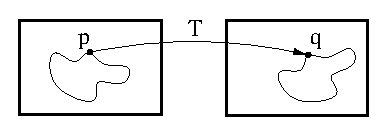
\includegraphics[width=8cm]{ImageRegistrationConcept.eps}}
  
This chapter introduces ITK's capabilities for performing image
registration. Image registration is the process of determining the spatial
transform that maps points from one image to homologous points on a object in
the second image. This concept is schematically represented in Figure
\ref{fig:ImageRegistrationConcept}. In ITK, registration is performed within
a framework of pluggable components that can easily be interchanged.  This
flexibility means that a combinatorial variety of registration methods can be
created, allowing users to pick and choose the right tools for their specific
application.


\section{Registration Framework}
The components of the registration framework and their interconnections are
shown in Figure \ref{fig:RegistrationComponents}. The basic input data to the
registration process are two images: one is defined as the \emph{fixed} image
$f(\bf{X})$ and the other as the \emph{moving} image $m(\bf{X})$. Where
$\bf{X}$ represents a position in N-dimensional space. Registration is treated
as an optimization problem with the goal of finding the spatial mapping that
will bring the moving image into alignment with the fixed image.

\begin{figure}
\center
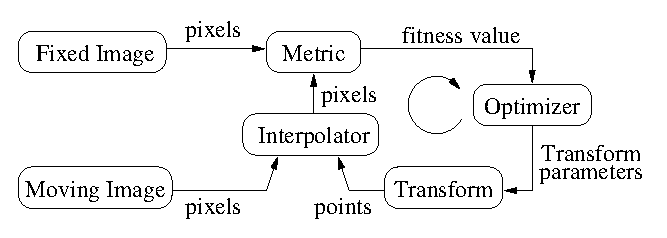
\includegraphics[width=0.8\textwidth]{RegistrationComponentsDiagram.eps}
\itkcaption[Registration Framework Components]{The basic components of the
registration framework are two input images, a transform, a metric, an
interpolator and an optimizer.}
\label{fig:RegistrationComponents}
\end{figure}

The \emph{transform} component $T(\bf{X})$ represents the spatial mapping of
points from the fixed image space to points in the moving image space. The
\emph{interpolator} is used to evaluate moving image intensities at non-grid
positions. The \emph{metric} component $S(f,m \circ T)$ provides a measure of
how well the fixed image is matched by the transformed moving image. This
measure forms the quantitative criterion to be optimized by the
\emph{optimizer} over the search space defined by the parameters of the
\emph{transform}.

These various ITK registration components will be described in later
sections.  First, we begin with some simple registration examples.

\section{"Hello World" Registration}
\label{sec:IntroductionImageRegistration}
\ifitkFullVersion
\input{ImageRegistration1.tex}
\fi

\section{Features of the Registration Framework}
\label{sec:FeaturesOfTheRegistrationFramework}

\begin{figure}
\center
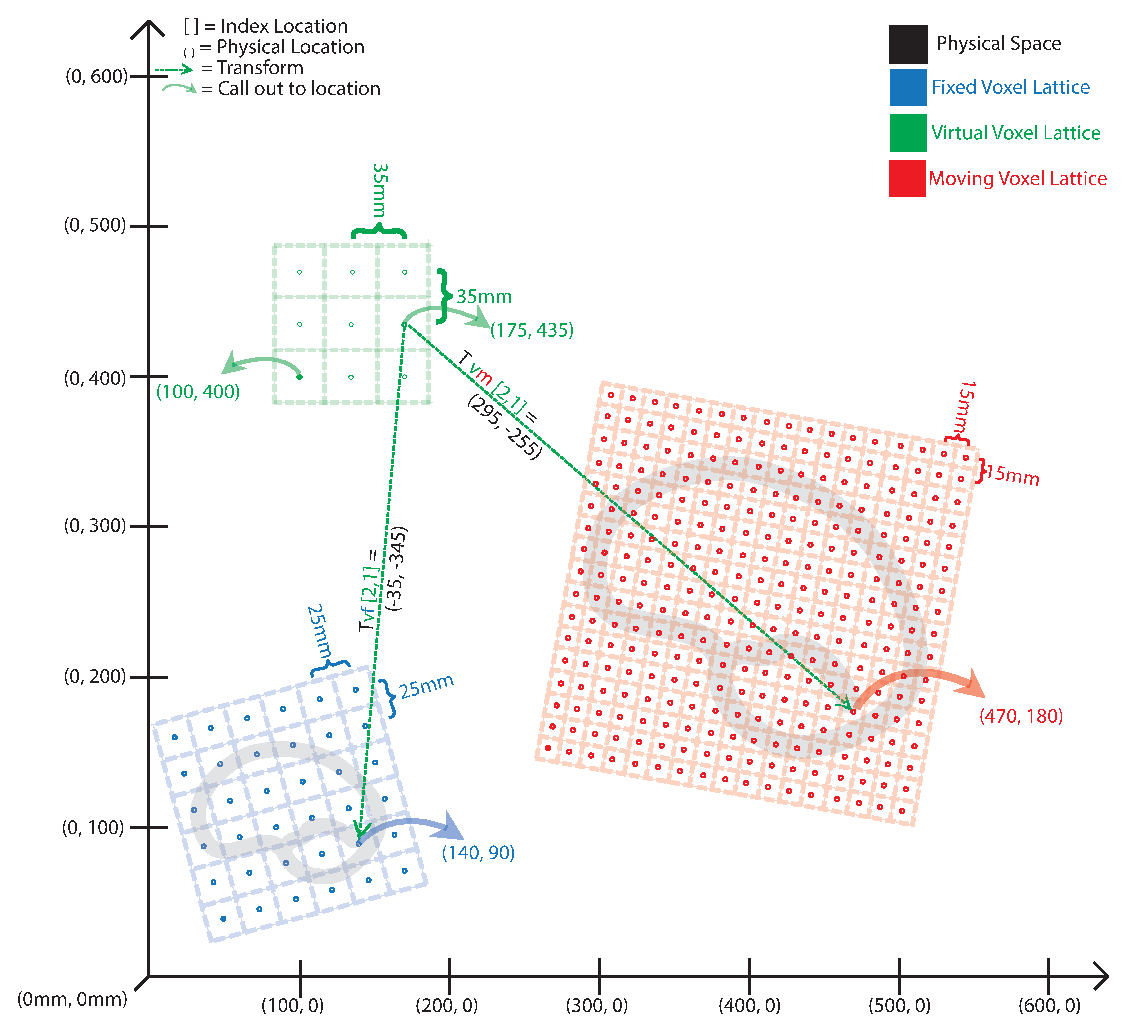
\includegraphics[width=0.75\textwidth]{ImageRegistrationCoordinateSystemsDiagram.eps}
\itkcaption[Registration Coordinate Systems]{Different coordinate systems
involved in the image registration process. Note that the transform being
optimized is the one mapping from the physical space of the fixed image
into the physical space of the moving image.}
\label{fig:ImageRegistrationCoordinateSystemsDiagram}
\end{figure}


This section presents a discussion on the two most common difficulties that
users encounter when they start using the ITK registration framework. They are,
in order of difficulty

\begin{itemize}
\item The direction of the Transform mapping
\item The fact that registration is done in physical coordinates
\end{itemize}

Probably the reason why these two topics tend to create confusion is that they
are implemented in different ways in other systems and therefore users tend to
have different expectations regarding how things should work in ITK. The
situation is further complicated by the fact that most people describe image
operations as if they were manually performed in a picture in paper.

\subsection{Direction of the Transform Mapping}
\label{sec:DirectionOfTheTransformMapping}

The Transform that is optimized in the ITK registration framework is the one
that maps points from the physical space of the fixed image into the physical
space of the moving image. This is illustrated in
Figure~\ref{fig:ImageRegistrationCoordinateSystemsDiagram}. This implies that
the Transform will accept as input points from the fixed image and it will
compute the coordinates of the analogous points in the moving image. What tends
to create confusion is the fact that when the Transform shifts a point on the
\textbf{positive} X direction, the visual effect of this mapping, once the
moving image is resampled, is equivalent to {\em manually shifting} the moving
image along the \textbf{negative} X direction. In the same way, when the
Transform applies a \textbf{clock-wise} rotation to the fixed image points, the
visual effect of this mapping once the moving image has been resampled is
equivalent to {\em manually rotating} the moving image
\textbf{counter-clock-wise}. 

The reason why this direction of mapping has been chosen for the ITK
implementation of the registration framework is that this is the direction that
better fits the fact that the moving image is expected to be resampled using
the grid of the fixed image. The nature of the resampling process is such that
an algorithm must go through every pixel of the {\em fixed} image and compute
the intensity that should be assigned to this pixel from the mapping of the
{\em moving} image. This computation involves taking the integral coordinates
of the pixel in the image grid, usually called the ``(i,j)'' coordinates,
mapping them into the physical space of the fixed image (transform \textbf{T1}
in Figure~\ref{fig:ImageRegistrationCoordinateSystemsDiagram}), mapping those
physical coordinates into the physical space of the moving image (Transform to
be optimized), then mapping the physical coordinates of the moving image in to
the integral coordinates of the discrete grid of the moving image (transform
\textbf{T2} in the figure), where the value of the pixel intensity will be
computed by interpolation. 

If we have used the Transform that maps coordinates from the moving image
physical space into the fixed image physical space, then the resampling process
could not guarantee that every pixel in the grid of the fixed image was going
to receive one and only one value. In other words, the resampling will have
resulted in an image with holes and with redundant or overlapped pixel values.

As you have seen in the previous examples, and you will corroborate in the
remaining examples in this chapter, the Transform computed by the registration
framework is the Transform that can be used directly in the resampling filter
in order to map the moving image into the discrete grid of the fixed image.

There are exceptional cases in which the transform that you want is actually
the inverse transform of the one computed by the ITK registration framework.
Only in those cases you may have to recur to invoking the \code{GetInverse()}
method that most transform offer.  Make sure that before you consider following
that dark path, you interact with the examples of resampling illustrated in
section~\ref{sec:GeometricalTransformationFilters} in order to get familiar
with the correct interpretation of the transforms.


\subsection{Registration is done in physical space}
\label{sec:RegistrationIsDoneInPhysicalSpace}

The second common difficulty that users encounter with the ITK registration
framework is related to the fact that ITK performs registration in the context
of physical space and not in the discrete space of the image grid.
Figure~\ref{fig:ImageRegistrationCoordinateSystemsDiagram} show this concept by
crossing the transform that goes between the two image grids. One important
consequence of this fact is that having the correct image origin and image
pixel size is fundamental for the success of the registration process in ITK.
Users must make sure that they provide correct values for the origin and
spacing of both the fixed and moving images.

A typical case that helps to understand this issue, is to consider the
registration of two images where one has a pixel size different from the other.
For example, a PET\footnote{Positron Emission Tomography} image and a
CT\footnote{Computer Tomography in X-rays} image. Typically a CT image will
have a pixel size in the order of 1 millimeter, while a PET image will have a
pixel size in the order of 5 millimeters to 1 centimeter. Therefore, the CT
will need about 500 pixels in order to cover the extent across a human brain, while
the PET image will only have about 50 pixels for covering the same physical
extent of a human brain. 

A user performing registration between a PET image and a CT image may be
naively expecting that because the PET image has less pixels, a {\em scaling}
factor is required in the Transform in order to map this image into the CT
image. At that point, this person is attempting to interpret the registration
process directly between the two image grids, or in {\em pixel space}. What ITK
will do in this case is to take into account the pixel size that the user has
provided and it will use that pixel size in order to compute a scaling factor
for Transforms {\em T1} and {\em T2} in
Figure~\ref{fig:ImageRegistrationCoordinateSystemsDiagram}. Since these two
transforms take care of the required scaling factor, the spatial Transform to
be computed during the registration process does not need to be concerned about
such scaling. The transform that ITK is computing is the one that will
physically map the brain from the moving image into the brain of the fixed
image.

In order to better understand this concepts, it is very useful to draw sketches
of the fixed and moving image {\em at scale} in the same physical coordinate
system. That is the geometrical configuration that the ITK registration
framework uses as context. Keeping this in mind helps a lot for interpreting
correctly the results of a registration process performed with ITK.

\section{Monitoring Registration}
\label{sec:MonitoringImageRegistration}
\ifitkFullVersion
\input{ImageRegistration3.tex}
\fi



\section{Multi-Modality Registration}
\label{sec:MultiModalityRegistration}

Some of the most challenging cases of image registration arise when images of
different modalities are involved. In such cases, metrics based on direct
comparison of gray levels are not applicable. It has been extensively shown
that metrics based on the evaluation of mutual information are well suited for
overcoming the difficulties of multi-modality registration.

\index{itk::Image\-Registration\-Method!Multi-Modality}

The concept of Mutual Information is derived from Information Theory and its
application to image registration has been proposed in different forms by
different groups \cite{Collignon1995,Maes97,Viola1997}, a more detailed review
can be found in \cite{Hajnal2001,Pluim2003}. The Insight Toolkit currently
provides five different implementations of Mutual Information metrics (see
section \ref{sec:Metrics} for details). The following examples illustrate the
practical use of some of these metrics.

\subsection{Viola-Wells Mutual Information}
\label{sec:MultiModalityRegistrationViolaWells}
\ifitkFullVersion
\input{ImageRegistration2.tex}
\fi

\subsection{Mattes Mutual Information}
\label{sec:MultiModalityRegistrationMattes}
\ifitkFullVersion
\input{ImageRegistration4.tex}
\fi


\subsection{Plotting joint histograms}
\label{sec:JointHistograms}
\ifitkFullVersion
\input{ImageRegistrationHistogramPlotter.tex}
\fi


\section{ Centered Transforms }

The ITK image coordinate origin is typically located in one of the image
corners (see section ~\ref{sec:DefiningImageOriginAndSpacing} for details).
This results in counter-intuitive transform behavior when rotations and scaling
are involved. Users tend to assume that rotations and scaling are performed
around a fixed point at the center of the image.  In order to compensate for
this difference in natural interpretation, the concept of \emph{centered}
transforms have been introduced into the toolkit. The following sections
describe the main characteristics of such transforms.

The introduction of the centered transforms in the Insight Toolkit reflects the
dynamic nature of a software library when it evolves in harmony with the
requests of the community that it serves. This dynamism has, as everything else
in real life, some advantages and some disavantages. The main advantage is that
when a need is identified by the users, it gets implemented in a matter of days
or weeks.  This capability for rapidly responding to the needs of a community
is one of the major strenghts of Open Source software. It has the additional
safety that if the rest of the community does not wish to adopt a particular
change, an isolated user can always implement that change in her local copy of
the toolkit, since all the source code of ITK is available in a BSD-style
license\footnote{\url{http://www.opensource.org/licenses/bsd-license.php}} that
does not restrict modification nor distribution of the code, and that does not
impose the assimilation demands of viral licenses such as
GPL\footnote{\url{http://www.gnu.org/copyleft/gpl.html}}.

The main disadvantage of dynamism, is of course, the fact that there is
continuous change and a need for perpetual adaptation. The evolution of
software occurs at different scales, some changes happen to evolve in localized
regions of the code, while from time to time acommodations of a larger scale
are needed. The need for continuos changes is addressed in Extreme Programming
with the methodology of \emph{Refactoring}. At any given point, the structure
of the code may not project the organized and neatly distributed architecture
that may have resulted from a monolithic and static design. There is, after
all, good reasons why living beings can not have straight angles. What you are
about to witness in this section is a clear example of the diversity of species
that flourishes when Evolution is in action~\cite{Darwin1999}.


\subsection{Rigid Registration in 2D}
\label{sec:RigidRegistrationIn2D}
\ifitkFullVersion
\input{ImageRegistration5.tex}
\fi

\subsection{Initializing with Image Moments}
\label{sec:InitializingRegistrationWithMoments}
\ifitkFullVersion
\input{ImageRegistration6.tex}
\fi



\subsection{Similarity Transform in 2D}
\label{sec:SimilarityRegistrationIn2D}
\ifitkFullVersion
\input{ImageRegistration7.tex}
\fi



\subsection{Rigid Transform in 3D}
\label{sec:RigidRegistrationIn3D}
\ifitkFullVersion
\input{ImageRegistration8.tex}
\fi




\subsection{Centered Affine Transform}
\label{sec:CenteredAffineTransform}
\ifitkFullVersion
\input{ImageRegistration9.tex}
\fi




\section{Multi-Resolution Registration}
\label{sec:MultiResolutionRegistration}
Performing image registration using a multi-resolution approach is widely used
to improve speed, accuracy and robustness. The basic idea is that registration
is first performed at a coarse scale where the images have fewer pixels.
The spatial mapping determined at the coarse level is then used to initialize
registration at the next finer scale. This process is repeated until it
reaches the finest possible scale. This coarse-to-fine strategy greatly
improve the registration success rate and also increases robustness
by eliminating local optima at coarser scales.

The Insight Toolkit offers a multi-resolution registration framework that is
directly compatible with all the registration framework components. The
multi-resolution registration framework has two additional components: a pair
of \emph{image pyramids} that are used to down-sample the fixed and moving
images as illustrated in Figure \ref{fig:MultiResRegistrationComponents}.
The pyramids smooth and subsample the images according to user-defined
scheduling of shrink factors.
 
\begin{figure}
\center
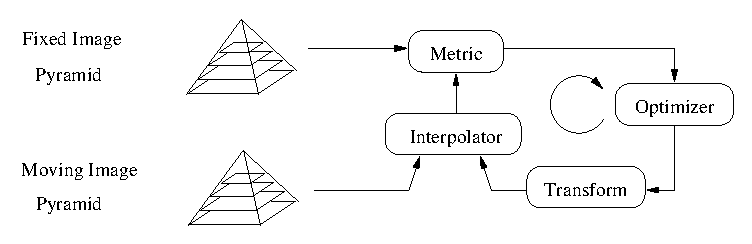
\includegraphics[width=0.8\textwidth]{MultiResRegistrationComponents.eps}
\itkcaption[Multi-Resolution Registration Components]{Components of the
multi-resolution registration framework.}
\label{fig:MultiResRegistrationComponents}
\end{figure}
 
We now present the main capabilities of the multi-resolution framework by
way of an example.

\subsection{Fundamentals}
\ifitkFullVersion
\input{MultiResImageRegistration1.tex}
\fi

\subsection{Parameter Tuning}
\ifitkFullVersion
\input{MultiResImageRegistration2.tex}
\fi

With the completion of these examples, we will now review the main
features of the components forming the registration framework.


% This clearpage command is intended to separate the graphics from previous
% examples from the diagrams of this section. This should prevent the
% registration diagrams from getting mixed with the diagrams for the Geometric
% objects used by the Transforms.
\clearpage

\section{Transforms}
\label{sec:Transforms}
\ifitkFullVersion

\def\tableconfiguration{ | p{3cm} | p{1.8cm} | p{2.5cm} | p{4cm} | }


\index{itk::Transform}

\index{Vector!Geometrical Concept}

In the Insight Toolkit, \doxygen{Transform} objects encapsulate the mapping of
points and vectors from an input space to an output space.  If a transform is
invertible, back transform methods are also provided.  Currently, ITK provides
a variety of transforms from simple translation, rotation and scaling to
general affine and kernel transforms.  Note that, while in this section we
discuss transforms in the context of registration, transforms are general and
can be used for other applications. Some of the most commonly used transforms
will be discussed in detail later. Let's begin by introducing the objects used
in ITK for representing basic spatial concepts.


\subsection{Geometrical Representation}
\label{sec:GeometricalObjects}

\begin{figure}
\center
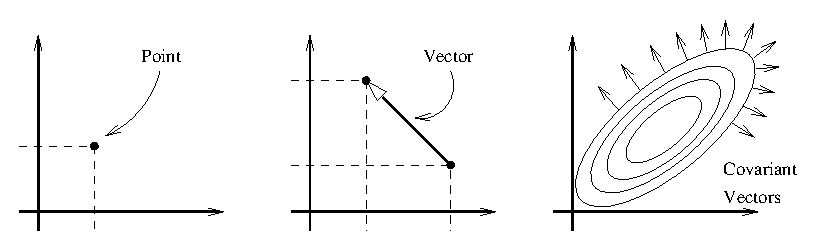
\includegraphics[width=0.9\textwidth]{GeometricalObjects.eps}
\itkcaption[Geometrical representation objects in ITK]{Geometric
representation objects in ITK.}
\label{fig:GeometricalObjects}
\end{figure}
 
ITK implements a consistent geometric representation of the space. The
characteristics of classes involved in this representation are summarized in
Table~\ref{tab:GeometricalConcepts}. In this regard, ITK takes full advantage
of the capabilities of Object Oriented programming and resists the temptation
of using simple arrays of \code{float} or \code{double} in order to represent
geometrical objects. The use of basic arrays would have blurred the important
distinction between the different geometrical concepts and would have allowed
for the innumerable conceptual and programming errors that result from using a
vector where a point is needed or viceversa.

\index{itk::Point!Concept}
\index{itk::Vector!Concept}
\index{itk::CovariantVector!Concept}

\begin{table}
\begin{center}
\begin{tabular}{ | p{0.3\textwidth} | p{ 0.6\textwidth} | }
\hline
\textbf{Class} &
\textbf{Geometrical concept} \\
\hline\hline
\doxygen{Point} & 
Position in space. In $N$-dimensional space it is represented by an array of
$N$ numbers associated with space coordinates. \\
\hline
\doxygen{Vector} & 
Relative position between two points. In $N$-dimensional space it is
represented by an array of $N$ numbers, each one associated with the distance
along a coordinate axis. Vectors do not have a position in space. A vector is
defined as the subtraction of two points.\\
\hline
\doxygen{CovariantVector} & Orthogonal direction to a $(N-1)$-dimensional
manifold in space. For example, in $3D$ it corresponds to the vector orthogonal
to a surface. This is the appropriate class for representing Gradients of
functions. Covariant vectors do not have a position in space. Covariant vector
should not be added to Points, nor to Vectors.\\
\hline
\end{tabular}
\end{center}
\itkcaption[Geometrical Elementary Objects]{Summary of objects representing
geometrical concepts in ITK.\label{tab:GeometricalConcepts}}
\end{table}


Additional uses of the \doxygen{Point}, \doxygen{Vector} and
\doxygen{CovariantVector} classes have been discussed in Chapter
\ref{sec:DataRepresentation}.  Each one of these classes behaves differently
under spatial transformations. It is therefore quite important to keep their
distinction clear. Figure
\ref{fig:GeometricalObjects} illustrates the differences between
these concepts.


\index{itk::Transform!TransformPoint()}
\index{itk::Transform!TransformVector()}
\index{itk::Transform!TransformCovariantVector()}

Transform classes provide different methods for mapping each one of
the basic space-representation objects.  Points, vectors and covariant vectors
are transformed using the methods \code{TransformPoint()},
\code{TransformVector()} and \code{TransformCovariantVector()} respectively.

One of the classes that deserve further comments is the \doxygen{Vector}. This
ITK class tend to be misinterpreted as a container of elements instead of a
geometrical object. This is a common misconception originated by the fact that
Computer Scientist and Software Engineers misuse the term ``Vector''.  The
actual word ``Vector'' is relatively young. It was coined by William Hamilton
in his book ``\emph{Elements of Quaternions}'' published in 1886
(post-mortem)\cite{Hamilton1866}.  In the same text Hamilton coined the terms:
``\emph{Scalar}'', ``\emph{Versor}'' and ``\emph{Tensor}''.  Although the
modern term of ``\emph{Tensor}'' is used in Calculus in a different sense of
what Hamilton defined in his book at the time~\cite{Dodson1997}.

A ``\emph{Vector}'' is, by definition, a mathematical object that embodies the
concept of ``direction in space''. Strictly speaking, a Vector describes the
relationship between two Points in space, and captures both their relative
distance and orientation.

Computer scientists and software engineers missused the term vector in order to
represent the concept of an ``Indexed Set''~\cite{Austern1999}.  Mechanical
Engineers and Civil Engineers, who deal with the real world of physical objects
will not commit this mistake and will keep the word ``\emph{Vector}'' attached
to a geometrical concept.  Biologists, on the other hand, will associate
``\emph{Vector}'' to a ``vehicle'' that allows them to direct something in a
particular direction, for example, a virus that allows them to insert pieces of
code into a DNA strand~\cite{Lodish2000}.

Textbooks in programming do not help to clarify those concepts and losely use
the term ``\emph{Vector}'' for the purpose of representing an ``Enumerated set
of common elements''. STL follows this trend and continue using the word
``\emph{Vector}'' for what it was not supposed to be
used~\cite{Austern1999,Alexandrescu2001}. Linear Algebra devoids the
``\emph{Vector}'' from its notion of Geometrical reality and makes it an
abstract set of numbers with arithmetic operations associated.

For those of you who are looking for the ``\emph{Vector}'' in the Software
Engineering sense, please look at the \doxygen{Array} and \doxygen{FixedArray}
classes that actually provide such functionalities. Additionally, the
\doxygen{VectorContainer} and \doxygen{MapContainer} classes may be of interest
too. These container classes are intended for algorithms that require to insert
and delete elements, and that may have large numbers of elements.

The Insight Toolkit deals with real objects that inhabit the physical space.
This is particularly true in the context of the image registration framework.
We chose to give the appropriate name to the mathematical objects that describe
geometrical relationships in N-Dimensional space. It is for this reason that we
explicitly make clear the distincion between Point, Vector and CovariantVector,
despite the fact that most people would be happy with a simple use of
\code{double[3]} for the three concepts and then will proceed to perform all
sort of conceptually flawed operations such as 

\begin{itemize}
\item Adding two Points
\item Dividing a Point by a Scalar
\item Adding a Covariant Vector to a Point
\item Adding a Covariant Vector to a Vector
\end{itemize}

In order to enforce the correct use of the Geometrical concepts in ITK we
organized these classes in a hierarchy that supports reuse of code and yet
compartamentalize the behavior of the individual classes.  The use of the
\doxygen{FixedArray} as base class of the \doxygen{Point}, the \doxygen{Vector}
and the \doxygen{CovariantVector} was a design decision based on calling things
by their correct name.

An \doxygen{FixedArray} is an enumerated collection with a fixed number of
elements. You can instantiate a fixed array of letters, or a fixed array of
images, or a fixed array of transforms, or a fixed array of geometrical shapes.
Therefore, the FixedArray only implements the functionality that is necesary to
access those enumerated elements. No assumptions can be made at this point on
any other operations required by the elements of the FixedArray, except the
fact of having a default constructor.

The \doxygen{Point} is a type that represents the spatial coordinates of a
spatial location. Based on geometrical concepts we defined the valid operations
of the Point class. In particular we made sure that no \code{operator+()} was
defined between Points, and that no \code{operator*( scalar )} nor
\code{operator/( scalar )} were defined for Points.

In other words, you could do in ITK operations such as:

\begin{itemize}
\item Vector  = Point - Point
\item Point  +=  Vector
\item Point  -=  Vector
\item Point  = BarycentricCombination( Point, Point )
\end{itemize}

and you cannot (because you \textbf{should not}) do operation such as

\begin{itemize}
\item Point = Point * Scalar    
\item Point = Point + Point    
\item Point = Point / Scalar  
\end{itemize}

The \doxygen{Vector} is, by Hamilton's definition, the subtraction between two
points. Therefore a Vector must satisfy the following basic operations:

\begin{itemize}
\item Vector = Point - Point
\item Point  = Point + Vector
\item Point  = Point - Vector
\item Vector = Vector + Vector
\item Vector = Vector - Vector
\end{itemize}

An \doxygen{Vector} object is intended to be instantiated over elements that
support matematical operation such as addition, subtraction and multiplication
by scalars.


\subsection{Transform General Properties}
\label{sec:TransformGeneralProperties}

\index{itk::Transform!SetParameters()} Each transform class typically has
several methods for setting its parameters.  For example,
\doxygen{Euler2DTransform} provides methods for specifying the offset,
angle, and the entire rotation matrix.  However, for use in the
registration framework, the parameters are represented by a flat
Array of doubles to facilitate communication with generic
optimizers. In the case of the Euler2DTransform, the transform is also
defined by three doubles: the first representing the angle, and the last two the
offset. The flat array of parameters is defined using \code{SetParameters()}. A
description of the parameters and their ordering is documented in the 
sections that follow.
 
In the context of registration, the transform parameters define the search
space for optimizers. That is, the goal of the optimization is to find the set
of parameters defining a transform that results in the best possible value of
an image metric. The more parameters a transform has, the longer its
computational time will be when used in a registration method since the
dimension of the search space will be equal to the number of transform
parameters.

\index{itk::Transform!GetJacobian()}

Another requirement that the registration framework imposes on the transform
classes is the computation of their Jacobians. In general, metrics require
the knowledge of the Jacobian in order to compute Metric derivatives.
The Jacobian is a matrix whose element are the partial derivatives of the
output point with respect to the array of parameters that defines the
transform:\footnote{Note that the term \emph{Jacobian} is also commonly used
for the matrix representing the derivatives of output point coordinates with
respect to input point coordinates. Sometimes the term is loosely used to
refer to the determinant of such a matrix.~\cite{Dodson1997}}

\begin{equation}
J=\left[ \begin{array}{cccc}
\frac{\partial x_{1}}{\partial p_{1}} & 
\frac{\partial x_{1}}{\partial p_{2}} & 
\cdots  & \frac{\partial x_{1}}{\partial p_{m}}\\
\frac{\partial x_{2}}{\partial p_{1}} & 
\frac{\partial x_{2}}{\partial p_{2}} & 
\cdots  & \frac{\partial x_{2}}{\partial p_{m}}\\
\vdots  & \vdots  & \ddots  & \vdots \\
\frac{\partial x_{n}}{\partial p_{1}} & 
\frac{\partial x_{n}}{\partial p_{2}} & 
\cdots  & \frac{\partial x_{n}}{\partial p_{m}}
\end{array}\right]
\end{equation}

where $\{p_i\}$ are the transform parameters and $\{x_i\}$ are the coordinates
of the output point.  Within this framework, the Jacobian is represented by an
\doxygen{Array2D} of doubles and is obtained from the transform by method
\code{GetJacobian()}. The Jacobian can be interpreted as a matrix that
indicates for a point in the input space how much its mapping on the output
space will change as a response to a small variation in one of the transform
parameters. Note that the values of the Jacobian matrix depend on the point in
the input space. So actually the Jacobian can be noted as $J(\bf{X})$, where
${\bf{X}}=\{x_i\}$. The use of transform Jacobians enables the efficient
computation of metric derivatives.  When Jacobians are not available, metrics
derivatives have to be computed using finite difference at a price of $2M$
evaluations of the metric value, where $M$ is the number of transform
parameters.

The following sections describe the main characteristics of the transform
classes available in ITK.

\subsection{Identity Transform}
\label{sec:IdentityTransform}
\index{itk::IdentityTransform}

\begin{table}
\begin{center}
\begin{tabular}{\tableconfiguration}
\hline
\textbf{Behavior} &
\textbf{Number of Parameters} &
\textbf{Parameter Ordering} &
\textbf{Restrictions} \\
\hline\hline
Maps every point to itself, every vector to itself and every covariant vector to itself.  & 
0 &
NA  &  
Only defined when the input and output space has the same number of dimensions. \\
\hline
\end{tabular}
\end{center}
\itkcaption[Identity Transform Characteristics]{Characteristics of the identity transform.
\label{tab:IdentityTransformCharacteristics}}
\end{table}

The identity transform \doxygen{IdentityTransform} is mainly used for debugging
purposes. It is provided to methods that require a transform and in cases where
we want to have the certainty that the transform will have no effect whatsoever
in the outcome of the process. It is just a \code{NULL} operation. The main
characteristics of the identity transform are summarized in
Table~\ref{tab:IdentityTransformCharacteristics}


\subsection{Translation Transform}
\label{sec:TranslationTransform}
\index{itk::TranslationTransform}

\begin{table}
\begin{center}
\begin{tabular}{\tableconfiguration}
\hline
\textbf{Behavior} &
\textbf{Number of Parameters} &
\textbf{Parameter Ordering} &
\textbf{Restrictions} \\
\hline\hline
Represents a simple translation of points in the input space
and has no effect on vectors or covariant vectors. &
Same as the input space dimension. &
The $i$-th parameter represents the translation in the $i$-th dimension. &
Only defined when the input and output space has the same number of dimensions. \\
\hline
\end{tabular}
\end{center}
\itkcaption[Translation Transform Characteristics]{Characteristics of the TranslationTransform class.
\label{tab:TranslationTransformCharacteristics}}
\end{table}

The \doxygen{TranslationTransform} is probably the simplest yet one of the most
useful transformations.  It maps all Points by adding a Vector to them.  Vector
and covariant vectors remain unchanged under this transformation since they are
not associated with a particular position in space. Translation is the best
transform to use when starting a registration method. Before attempting to
solve for rotations or scaling it is important to overlap the anatomical
objects in both images as much as possible. This is done by resolving the
translational misalignment between the images. Translations also have the
advantage of being fast to compute and having parameters that are easy to
interpret. The main characteristics of the translation transform are presented
in Table~\ref{tab:TranslationTransformCharacteristics}.

\subsection{Scale Transform}
\label{sec:ScaleTransform}
\index{itk::ScaleTransform}

\begin{table}
\begin{center}
\begin{tabular}{\tableconfiguration}
\hline
\textbf{Behavior} &
\textbf{Number of Parameters} &
\textbf{Parameter Ordering} &
\textbf{Restrictions} \\
\hline\hline
Points are transformed by multiplying each one of their coordinates by the
corresponding scale factor for the dimension.  Vectors are transformed as
points.  Covariant vectors are transformed by \emph{dividing} their components
by the scale factor in the corresponding dimension.  &
Same as the input space dimension. &
The $i$-th parameter represents the scaling in the $i$-th dimension. &
Only defined when the input and output space has the same number of dimensions. \\
\hline
\end{tabular}
\end{center}
\itkcaption[Scale Transform Characteristics]{Characteristics of the ScaleTransform class.
\label{tab:ScaleTransformCharacteristics}}
\end{table}

The \doxygen{ScaleTransform} represents a simple scaling of the
vector space.  Different scaling factors can be applied along each
dimension. Points are transformed by multiplying each one of their
coordinates by the corresponding scale factor for the dimension.  Vectors are
transformed in the same way as points.  Covariant vectors, on the other hand,
are transformed differently since anisotropic scaling does not preserve
angles. Covariant vectors are transformed by \emph{dividing} their components
by the scale factor of the corresponding dimension. In this way, if a
covariant vector was orthogonal to a vector, this orthogonality will be
preserved after the transformation. The following equations summarize the
effect of the transform on the basic geometric objects.

\begin{equation}
\begin{array}{lccccccc}
\mbox{Point }          & \bf{P'} &  =  & T(\bf{P})  & : & \bf{P'}_i &  = & \bf{P}_i \cdot S_i \\
\mbox{Vector}          & \bf{V'} &  =  & T(\bf{V})  & : & \bf{V'}_i &  = & \bf{V}_i \cdot S_i \\
\mbox{CovariantVector} & \bf{C'} &  =  & T(\bf{C})  & : & \bf{C'}_i &  = & \bf{C}_i /     S_i \\
\end{array}
\end{equation}

where $\bf{P}_i$, $\bf{V}_i$ and $\bf{C}_i$ are the point, vector and covariant
vector $i$-th components while $\bf{S}_i$ is the scaling factor along dimension
$i-th$.  The following equation illustrates the effect of the scaling transform
on a $3D$ point.

\begin{equation}
\left[ 
\begin{array}{c}
x' \\
y' \\
z' \\
\end{array}
\right]
=
\left[ 
\begin{array}{ccc}
S_1 &  0  &  0  \\
 0  & S_2 &  0  \\
 0  &  0  & S_3 \\
\end{array}
\right]
\cdot
\left[ 
\begin{array}{c}
x  \\
y  \\
z  \\
\end{array}
\right]
\end{equation}

Scaling appears to be a simple transformation but there are actually a
number of issues to keep in mind when using different scale factors along
every dimension. There are subtle effects---for example, when computing image
derivatives. Since derivatives are represented by covariant vectors, their
values are not intuitively modified by scaling transforms.

One of the difficulties with managing scaling transforms in a registration
process is that typical optimizers manage the parameter space as a vector
space where addition is the basic operation. Scaling is better treated in the
frame of a logarithmic space where additions result in regular multiplicative
increments of the scale. Gradient descent optimizers have trouble updating
step length, since the effect of an additive increment on a scale factor
diminishes as the factor grows. In other words, a scale factor variation of
$(1.0+ \epsilon)$ is quite different from a scale variation of
$(5.0+\epsilon)$.

Registrations involving scale transforms require careful monitoring of the
optimizer parameters in order to keep it progressing at a stable pace. Note
that some of the transforms discussed in following sections, for example, the
AffineTransform, have hidden scaling parameters and are therefore
subject to the same vulnerabilities of the ScaleTransform.

In cases involving misalignments with simultaneous translation, rotation and
scaling components it may be desirable to solve for these components
independently. The main characteristics of the scale transform are presented in
Table~\ref{tab:ScaleTransformCharacteristics}.


\subsection{Scale Logarithmic Transform}
\label{sec:ScaleLogarithmicTransform}
\index{itk::ScaleLogarithmicTransform}

\begin{table}
\begin{center}
\begin{tabular}{\tableconfiguration}
\hline
\textbf{Behavior} &
\textbf{Number of Parameters} &
\textbf{Parameter Ordering} &
\textbf{Restrictions} \\
\hline\hline
Points are transformed by multiplying each one of their coordinates by the
corresponding scale factor for the dimension.  Vectors are transformed as
points.  Covariant vectors are transformed by \emph{dividing} their components
by the scale factor in the corresponding dimension. 
&
Same as the input space dimension. &
The $i$-th parameter represents the scaling in the $i$-th dimension. &
Only defined when the input and output space has the same number of dimensions.
The difference between this transform and the ScaleTransform is that here the
scaling factors are passed as logarithms, in this way their behavior is closer
to the one of a Vector space.  \\
\hline
\end{tabular}
\end{center}
\itkcaption[Scale Logarithmic Transform Characteristics]{Characteristics of the ScaleLogarithmicTransform class.
\label{tab:ScaleLogarithmicTransformCharacteristics}}
\end{table}

The \doxygen{ScaleLogarithmicTransform} is a simple variation of the
\doxygen{ScaleTransform}. It is intended to improve the behavior of the scaling
parameters when they are modified by optimizers. The difference between this
transform and the ScaleTransform is that the parameter factors are passed here
as logarithms. In this way, multiplicative variations in the scale become
additive variations in the logarithm of the scaling factors.




\subsection{Euler2DTransform}
\label{sec:Euler2DTransform}
\index{itk::Euler2DTransform}

\begin{table}
\begin{center}
\begin{tabular}{\tableconfiguration}
\hline
\textbf{Behavior} &
\textbf{Number of Parameters} &
\textbf{Parameter Ordering} &
\textbf{Restrictions} \\
\hline\hline
Represents a $2D$ rotation and a $2D$ translation. Note that the translation
component has no effect on the transformation of vectors and covariant vectors. &
3 &
The first parameter is the angle in radians and the last two parameters
are the translation in each dimension. &
Only defined for two-dimensional input and output spaces. \\
\hline
\end{tabular}
\end{center}
\itkcaption[Euler2D Transform Characteristics]{Characteristics of the Euler2DTransform class.
\label{tab:Euler2DTransformCharacteristics}}
\end{table}

\doxygen{Euler2DTransform} implements a rigid transformation in $2D$. It is 
composed of a plane rotation and a two-dimensional translation. The rotation
is applied first, followed by the translation. The following equation
illustrates the effect of this transform on a $2D$ point,


\begin{equation}
\left[ 
\begin{array}{c}
x' \\
y' \\
\end{array}
\right]
=
\left[ 
\begin{array}{cc}
\cos{\theta} & -\sin{\theta} \\
\sin{\theta} &  \cos{\theta} \\
\end{array}
\right]
\cdot
\left[ 
\begin{array}{c}
x  \\
y  \\
\end{array}
\right]
+ 
\left[ 
\begin{array}{c}
T_x  \\
T_y  \\
\end{array}
\right]
\end{equation}

where $\theta$ is the rotation angle and $(T_x,T_y)$ are the components of the
translation.

A challenging aspect of this transformation is the fact that translations and
rotations do not form a vector space and cannot be managed as linear
independent parameters. Typical optimizers make the loose assumption that
parameters exist in a vector space and rely on the step length to be small
enough for this assumption to hold approximately.

In addition to the non-linearity of the parameter space, the most common
difficulty found when using this transform is the difference in units used
for rotations and translations. Rotations are measured in radians; hence,
their values are in the range $[-\pi,\pi]$. Translations are measured in
millimeters and their actual values vary depending on the image modality
being considered. In practice, translations have values on the order of $10$
to $100$. This scale difference between the rotation and translation
parameters is undesirable for gradient descent optimizers because they
deviate from the trajectories of descent and make optimization slower and more
unstable. In order to compensate for these differences, ITK optimizers accept
an array of scale values that are used to normalize the parameter space.

Registrations involving angles and translations should take advantage of the
scale normalization functionality in order to obtain the best performance out
of the optimizers. The main characteristics of the Euler2DTransform class
are presented in Table~\ref{tab:Euler2DTransformCharacteristics}.


\subsection{CenteredRigid2DTransform}
\label{sec:CenteredRigid2DTransform}
\index{itk::CenteredRigid2DTransform}

\begin{table}
\begin{center}
\begin{tabular}{\tableconfiguration}
\hline
\textbf{Behavior} &
\textbf{Number of Parameters} &
\textbf{Parameter Ordering} &
\textbf{Restrictions} \\
\hline\hline
Represents a $2D$ rotation around a user-provided center followed by a $2D$ translation.&
5 &
The first parameter is the angle in radians. Second and third are the center of
rotation coordinates and the last two parameters are the translation in each
dimension. & 
Only defined for two-dimensional input and output spaces. \\
\hline
\end{tabular}
\end{center}
\itkcaption[CenteredRigid2D Transform Characteristics]{Characteristics of the CenteredRigid2DTransform class.
\label{tab:CenteredRigid2DTransformCharacteristics}}
\end{table}

\doxygen{CenteredRigid2DTransform} implements a rigid transformation in $2D$.
The main difference between this transform and the \doxygen{Euler2DTransform}
is that here we can specify an arbitrary center of rotation, while the
Euler2DTransform always uses the origin of the coordinate system as the center
of rotation. This distinction is quite important in image registration since
ITK images usually have their origin in the corner of the image rather than the
middle.  Rotational mis-registrations usually exist, however, as rotations
around the center of the image, or at least as rotations around a point in the
middle of the anatomical structure captured by the image. Using gradient
descent optimizers, it is almost imposible to solve non-origin rotations using
a transform with origin rotations since the deep basin of the real solution is
usually located across a high ridge in the topography of the cost function.

In practice, the user must supply the center of rotation in the input space,
the angle of rotation and a translation to be applied after the rotation. With
these parameters, the transform initializes a rotation matrix and a translation
vector that together perform the equivalent of translating the center of
rotation to the origin of coordinates, rotating by the specified angle,
translating back to the center of rotation and finally translating by the
user-specified vector.

As with the Euler2DTransform, this transform suffers from the difference in
units used for rotations and translations. Rotations are measured in radians;
hence, their values are in the range $[-\pi,\pi]$. The center of rotation and
the translations are measured in millimeters, and their actual values vary
depending on the image modality being considered.  Registrations involving
angles and translations should take advantage of the scale normalization
functionality of the optimizers in order to get the best performance out of
them.

The following equation illustrates the effect of the transform on an input
point $(x,y)$ that maps to the output point $(x',y')$,

\begin{equation}
\left[ 
\begin{array}{c}
x' \\
y' \\
\end{array}
\right]
=
\left[ 
\begin{array}{cc}
\cos{\theta} & -\sin{\theta} \\
\sin{\theta} &  \cos{\theta} \\
\end{array}
\right]
\cdot
\left[ 
\begin{array}{c}
x - C_x \\
y - C_y \\
\end{array}
\right]
+ 
\left[ 
\begin{array}{c}
T_x + C_x \\
T_y + C_y \\
\end{array}
\right]
\end{equation}

where $\theta$ is the rotation angle, $(C_x,C_y)$ are the coordinates of the
rotation center and $(T_x,T_y)$ are the components of the translation. Note
that the center coordinates are subtracted before the rotation and added back
after the rotation. The main features of the CenteredRigid2DTransform are 
presented in Table~\ref{tab:CenteredRigid2DTransformCharacteristics}.


\subsection{Similarity2DTransform}
\label{sec:Similarity2DTransform}
\index{itk::Similarity2DTransform}

\begin{table}
\begin{center}
\begin{tabular}{\tableconfiguration}
\hline
\textbf{Behavior} &
\textbf{Number of Parameters} &
\textbf{Parameter Ordering} &
\textbf{Restrictions} \\
\hline\hline
Represents a $2D$ rotation, homogeneous scaling and a $2D$ translation. Note that
the translation component has no effect on the transformation of vectors and
covariant vectors. & 
4 &
The first parameter is the scaling factor for all dimensions, the second is the
angle in radians, and the last two parameters are the translations in $(x,y)$
respectively. & 
Only defined for two-dimensional input and output spaces. \\
\hline
\end{tabular}
\end{center}
\itkcaption[Similarity2D Transform Characteristics]{Characteristics of the Similarity2DTransform class.
\label{tab:Similarity2DTransformCharacteristics}}
\end{table}

The \doxygen{Similarity2DTransform} can be seen as a rigid transform combined
with an isotropic scaling factor. This transform preserves angles between
lines. In its $2D$ implementation, the four parameters of this transformation
combine the characteristics of the \doxygen{ScaleTransform} and
\doxygen{Euler2DTransform}. In particular, those relating to the non-linearity
of the parameter space and the non-uniformity of the measurement units.
Gradient descent optimizers should be used with caution on such parameter
spaces since the notions of gradient direction and step length are ill-defined.

The following equation illustrates the effect of the transform on an input
point $(x,y)$ that maps to the output point $(x',y')$,

\begin{equation}
\left[ 
\begin{array}{c}
x' \\
y' \\
\end{array}
\right]
=
\left[ 
\begin{array}{cc}
\lambda &    0     \\
   0    &  \lambda \\
\end{array}
\right]
\cdot
\left[ 
\begin{array}{cc}
\cos{\theta} & -\sin{\theta} \\
\sin{\theta} &  \cos{\theta} \\
\end{array}
\right]
\cdot
\left[ 
\begin{array}{c}
x - C_x \\
y - C_y \\
\end{array}
\right]
+ 
\left[ 
\begin{array}{c}
T_x + C_x \\
T_y + C_y \\
\end{array}
\right]
\end{equation}

where $\lambda$ is the scale factor, $\theta$ is the rotation angle,
$(C_x,C_y)$ are the coordinates of the rotation center and $(T_x,T_y)$ are the
components of the translation. Note that the center coordinates are subtracted
before the rotation and scaling, and they are added back afterwards.  The main
features of the Similarity2DTransform are presented in
Table~\ref{tab:Similarity2DTransformCharacteristics}.


A possible approach for controlling optimization in the parameter space of
this transform is to dynamically modify the array of scales passed to the
optimizer. The effect produced by the parameter scaling can be used to steer
the walk in the parameter space (by giving preference to some of the
parameters over others). For example, perform some iterations updating only
the rotation angle, then balance the array of scale factors in the optimizer
and perform another set of iterations updating only the translations.


\subsection{QuaternionRigidTransform}
\label{sec:QuaternionRigidTransform}
\index{itk::QuaternionRigidTransform}

\begin{table}
\begin{center}
\begin{tabular}{| p{4cm} | p{1.8cm} | p{2.5cm} | p{3cm} |}
\hline
\textbf{Behavior} &
\textbf{Number of Parameters} &
\textbf{Parameter Ordering} &
\textbf{Restrictions} \\
\hline\hline
Represents a $3D$ rotation and a $3D$ translation. The rotation is specified as a
quaternion, defined by a set of four numbers $\bf{q}$.  The relationship
between quaternion and rotation about vector $\bf{n}$ by angle $\theta$ is as
follows: \[ \bf{q} = (\bf{n}\sin(\theta/2), \cos(\theta/2))\] Note that if the
quaternion is not of unit length, scaling will also result. &
7 &
The first four parameters defines the quaternion and the last three parameters
the translation in each dimension. &
Only defined for three-dimensional input and output spaces. \\
\hline
\end{tabular}
\end{center}
\itkcaption[QuaternionRigid Transform Characteristics]{Characteristics of the QuaternionRigidTransform class.
\label{tab:QuaternionRigidTransformCharacteristics}}
\end{table}

The \doxygen{QuaternionRigidTransform} class implements a rigid
transformation in $3D$ space. The rotational part of the transform is
represented using a quaternion while the translation is represented with a
vector. Quaternions components do not form a vector space and hence raise the
same concerns as the \doxygen{Similarity2DTransform} when used with gradient
descent optimizers.

The \doxygen{QuaternionRigidTransformGradientDescentOptimizer} was introduced into the toolkit to address these concerns.  This specialized optimizer implements a variation of a
gradient descent algorithm adapted for a quaternion space.  This class
insures that after advancing in any direction on the parameter space, the
resulting set of transform parameters is mapped back into the permissible
set of parameters. In practice, this comes down to normalizing the newly-computed quaternion to make sure that the transformation remains rigid and no
scaling is applied.  The main characteristics of the
QuaternionRigidTransform are presented in
Table~\ref{tab:QuaternionRigidTransformCharacteristics}.

The Quaternion rigid transform also accepts a user-defined center of rotation.
In this way, the transform can easily be used for registering images where the
rotation is mostly relative to the center of the image instead one of the
corners. The coordinates of this rotation center are not subject to
optimization. They only participate in the computation of the mappings for
Points and in the computation of the Jacobian. The transformations for Vectors
and CovariantVector are not affected by the selection of the rotation center.



\subsection{VersorTransform}
\label{sec:VersorTransform}
\index{itk::VersorTransform}
\index{itk::VersorTransformOptimizer}
\index{itk::Versor!Definition}

\begin{table}
\begin{center}
\begin{tabular}{\tableconfiguration}
\hline
\textbf{Behavior} &
\textbf{Number of Parameters} &
\textbf{Parameter Ordering} &
\textbf{Restrictions} \\
\hline\hline
Represents a $3D$ rotation. The rotation is specified by a versor or unit
quaternion. The rotation is performed around a user-specified center of
rotation.&
3 &
The three parameters define the versor.&
Only defined for three-dimensional input and output spaces. \\
\hline
\end{tabular}
\end{center}
\itkcaption[Versor Transform Characteristics]{Characteristics of the Versor Transform
\label{tab:VersorTransformCharacteristics}}
\end{table}


By definition, a \emph{Versor} is the rotational part of a Quaternion. It can
also be defined as a \emph{unit-quaternion} \cite{Hamilton1866,Joly1905}.
Versors only have three independent components, since they are restricted to
reside in the space of unit-quaternions. The implementation of versors in the
toolkit uses a set of three numbers.  These three numbers correspond to the
first three components of a quaternion.  The fourth component of the quaternion
is computed internally such that the quaternion is of unit length. The main
characteristics of the \doxygen{VersorTransform} are presented in
Table~\ref{tab:VersorTransformCharacteristics}.

This transform exclusively represents rotations in $3D$. It is intended to
rapidly solve the rotational component of a more general misalignment.  The
efficiency of this transform comes from using a parameter space of reduced
dimensionality. Versors are the best possible representation for rotations in
$3D$ space. Sequences of versors allow the creation of smooth rotational
trajectories; for this reason, they behave stably under optimization methods.

The space formed by versor parameters is not a vector space. Standard gradient
descent algorithms are not appropriate for exploring this parameter space. An
optimizer specialized for the versor space is available in the toolkit under
the name of \doxygen{VersorTransformOptimizer}. This optimizer implements
versor derivatives as originally defined by Hamilton \cite{Hamilton1866}.

The center of rotation can be especified by the user with the
\code{SetCenter()} method. The center is not part of the parameters to be
optimized, therefore it remains the same during an optimization process. Its
value is used during the computations for transforming Points and when
computing the Jacobian.

\subsection{VersorRigid3DTransform}
\label{sec:VersorRigid3DTransform}
\index{itk::VersorRigid3DTransform}

\begin{table}
\begin{center}
\begin{tabular}{\tableconfiguration}
\hline
\textbf{Behavior} &
\textbf{Number of Parameters} &
\textbf{Parameter Ordering} &
\textbf{Restrictions} \\
\hline\hline
Represents a $3D$ rotation and a $3D$ translation. The rotation is specified by
a versor or unit quaternion, while the translation is represented by a vector.
Users can specify the coordinates of the center of rotation. &
6 &
The first three parameters define the versor and the last three parameters the
translation in each dimension. &
Only defined for three-dimensional input and output spaces. \\
\hline
\end{tabular}
\end{center}
\itkcaption[Versor Rigid3D Transform Characteristics]{Characteristics of the VersorRigid3DTransform class.
\label{tab:VersorRigid3DTransformCharacteristics}}
\end{table}

The \doxygen{VersorRigid3DTransform} implements a rigid transformation in $3D$
space. It is a variant of the \doxygen{QuaternionRigidTransform} and the
\doxygen{VersorTransform}. It can be seen as a \doxygen{VersorTransform} plus a
translation defined by a vector. The advantage of this class with respect to
the QuaternionRigidTransform is that it exposes only six parameters, three for
the versor components and three for the translational components. This reduces
the search space for the optimizer to six dimensions instead of the seven
dimensional used by the QuaternionRigidTransform.  This transform also allows
the users to set a specific center of rotation. The center coodinates are not
modified during the optimization performed in a registration process.  The main
features of this transform are summarized in
Table~\ref{tab:VersorRigid3DTransformCharacteristics}.  This transform is
probably the best option to use when dealing with rigid transformations in
$3D$. 

Given that the space of Versors is not a Vector space, typical gradient descent
optimizers are not well suited for exploring the parametric space of this
transform. The \doxygen{VersorRigid3DTranformOptimizer} has been
introduced in the ITK toolkit with the purpose of providing an optimizer that
is aware of the Versor space properties on the rotational part of this
transform, as well as the Vector space properties on the translational part of
the transform.


\subsection{Euler3DTransform}
\label{sec:Euler3DTransform}
\index{itk::Euler3DTransform}

\begin{table}
\begin{center}
\begin{tabular}{\tableconfiguration}
\hline
\textbf{Behavior} &
\textbf{Number of Parameters} &
\textbf{Parameter Ordering} &
\textbf{Restrictions} \\
\hline\hline
Represents a rigid rotation in $3D$ space. That is, a rotation followed by a
$3D$ translation. The rotation is specified by three angles representing
rotations to be applied around the X, Y and Z axis one after another.  The
translation part is represented by a Vector. Users can also specify the
coordinates of the center of rotation. &
6 &
The first three parameters are the rotation angles around X, Y and Z axis, and
the last three parameters are the translations along each dimension. &
Only defined for three-dimensional input and output spaces. \\
\hline
\end{tabular}
\end{center}
\itkcaption[Euler3D Transform Characteristics]{Characteristics of the Euler3DTransform class.
\label{tab:Euler3DTransformCharacteristics}}
\end{table}

The \doxygen{Euler3DTransform} implements a rigid transformation in $3D$ space.
It can be seen as a rotation followed by a translation. This class exposes six
parameters, three for the Euler angles that represent the rotation and three
for the translational components. This transform also allows the users to set a
specific center of rotation. The center coodinates are not modified during the
optimization performed in a registration process. The main features of this
transform are summarized in Table~\ref{tab:Euler3DTransformCharacteristics}.  

The fact that the three rotational parameters are non-linears and do not behave
like Vector spaces must be taken into account when selecting an optimizer to
work with this transform and when fine tunning the parameters of such
optimizer. It is strongly recommended to use this transform by introducing very
small variations on the rotaional components. A small rotation will be in the
range of 1 degree, which in radians is approximately $0.0.1745$.

You should not expect this transform to be able to compensate for large
rotations just by being driven with the optimizer. In practice you must provide
a reasonable initialization of the transform angles and only need to correct
for residual rotations in the order of $10$ or $20$ degrees.


\subsection{Similarity3DTransform}
\label{sec:Similarity3DTransform}
\index{itk::Similarity3DTransform}

\begin{table}
\begin{center}
\begin{tabular}{\tableconfiguration}
\hline
\textbf{Behavior} &
\textbf{Number of Parameters} &
\textbf{Parameter Ordering} &
\textbf{Restrictions} \\
\hline\hline
Represents a $3D$ rotation, a $3D$ translation and homogeneous scaling. The
scaling factor is specified by a scalar, the rotation is specified by a versor,
and the translation is represented by a vector.  Users can also specify the
coordinates of the center of rotation, that is the same center used for
scaling. &
7 &
The first parameter is the scaling factor, the next three parameters define the
versor and the last three parameters the translation in each dimension. &
Only defined for three-dimensional input and output spaces. \\
\hline
\end{tabular}
\end{center}
\itkcaption[Similarity3D Transform Characteristics]{Characteristics of the Similarity3DTransform class.
\label{tab:Similarity3DTransformCharacteristics}}
\end{table}

The \doxygen{Similarity3DTransform} implements a similarity transformation in
$3D$ space. It can be seen as an homogeneous scaling followed by a
\doxygen{VersorRigid3DTransform}. This class exposes seven parameters, one for
the scaling factor, three for the versor components and three for the
translational components. This transform also allows the users to set a
specific center of rotation. The center coodinates are not modified during the
optimization performed in a registration process.  Both the rotation and
scaling operations are performed with respect to the center of rotation. The
main features of this transform are summarized in
Table~\ref{tab:Similarity3DTransformCharacteristics}.  

The fact that the scaling and rotational spaces are non-linears and do not
behave like Vector spaces must be taken into account when selecting an
optimizer to work with this transform and when fine tunning the parameters of
such optimizer.


\subsection{Rigid3DPerspectiveTransform}
\label{sec:Rigid3DPerspectiveTransform}
\index{itk::Rigid3DPerspectiveTransform}

\begin{table}
\begin{center}
\begin{tabular}{\tableconfiguration}
\hline
\textbf{Behavior} &
\textbf{Number of Parameters} &
\textbf{Parameter Ordering} &
\textbf{Restrictions} \\
\hline\hline 
Represents a rigid $3D$ transformation followed by a perspective projection.
The rotation is specified by a Versor, while the translation is represented by
a Vector.  Users can specify the coordinates of the center of rotation. They
must specifiy a focal distance to be used for the perspective projection. The
rotation center and the focal distance parameters are not modified during the
optimization process. &
6 &
The first three parameters define the Versor and the last three parameters the
Translation in each dimension. &
Only defined for three-dimensional input and two-dimensional output spaces.
This is one of the few transforms where the input space has a different
dimension from the output space.\\
\hline
\end{tabular}
\end{center}
\itkcaption[Rigid3DPerspective Transform Characteristics]{Characteristics of
the Rigid3DPerspectiveTransform class.
\label{tab:VersorRigid3DTransformCharacteristics}}
\end{table}

The \doxygen{Rigid3DPerspectiveTransform} implements a rigid transformation in
$3D$ space followed by a perspective projection. This transform is intended to
be used in $3D/2D$ registration problems where a 3D object is projected onto a
2D plane. This is the case of Fluoroscopic images used for image guided
intervention, and it is also the case for classical radiography.  Users must
provide a value for the focal distance to be used during the computation of the
perspective transform. This transform also allows users to set a specific
center of rotation. The center coodinates are not modified during the
optimization performed in a registration process.  The main features of this
transform are summarized in
Table~\ref{tab:VersorRigid3DTransformCharacteristics}.  This transform is also
used when creating Digitally Reconstructed Radiographs (DRRs).

The strategies for optimizing the parameters of this transform are the same
ones used for optimizing the VersorRigid3DTransform. In particular, you can use
the same Versor\-Rigid3D\-Tranform\-Optimizer in order to optimize the
parameters of this class.


\subsection{AffineTransform}
\label{sec:AffineTransform}
\index{itk::AffineTransform}

\begin{table}
\begin{center}
\begin{tabular}{\tableconfiguration}
\hline
\textbf{Behavior} &
\textbf{Number of Parameters} &
\textbf{Parameter Ordering} &
\textbf{Restrictions} \\
\hline\hline
Represents an affine transform composed of rotation, scaling, shearing and
translation. The transform is specified by a $N \times N$ matrix and a $N
\times 1$ vector where $N$ is the space dimension. &
$(N+1) \times N$ &
The first $N \times N$ parameters define the matrix in column-major order
(where the column index varies the fastest).  The last $N$ parameters define
the translations for each dimension. &
Only defined when the input and output space have the same dimension. \\
\hline
\end{tabular}
\end{center}
\itkcaption[Affine Transform Characteristics]{Characteristics of the AffineTransform class.
\label{tab:AffineTransformCharacteristics}}
\end{table}

The \doxygen{AffineTransform} is one of the most popular transformations used
for image registration. Its main advantage comes from the fact that it is 
represented as a linear transformation. The main features of this
transform are presented in Table~\ref{tab:AffineTransformCharacteristics}.

The set of AffineTransform coefficients can actually be represented in a vector
space of dimension $(N+1) \times N$. This makes it possible for optimizers to
be used appropriately on this search space. However, the high dimensionality of
the search space also implies a high computational complexity of cost-function
derivatives. The best compromise in the reduction of this computational time is
to use the transform's Jacobian in combination with the image gradient for
computing the cost-function derivatives.

The coefficients of the $N \times N$ matrix can represent rotations,
anisotropic scaling and shearing. These coefficients are usually of a very
different dynamic range compared to the translation
coefficients. Coefficients in the matrix tend to be in the range $[-1:1]$, but
are not restricted to this interval.  Translation coefficients, on the other
hand, can be on the order of $10$ to $100$, and are basically related to the
image size and pixel spacing.

This difference in scale makes it necessary to take advantage of the
functionality offered by the optimizers for rescaling the parameter space. This
is particularly relevant for optimizers based on gradient descent approaches.

A registration based on the affine transform may be more effective when
applied after simpler transformations have been used to remove the major
components of misalignment. Otherwise it will incur an overwhelming
computational cost. For example, using an affine transform, the first set of
optimization iterations would typically focus on removing large
translations. This task could instead be accomplished by a translation
transform in a parameter space of size $N$ instead of the $(N+1) \times N$
associated with the affine transform.

Tracking the evolution of a registration process that uses
AffineTransforms can be challenging, since it is difficult to
represent the coefficients in a meaningful way.  A simple printout of the
transform coefficients generally does not offer a clear picture of the current
behavior and trend of the optimization.  A better implementation uses
the affine transform to deform wire-frame cube which is shown in a $3D$
visualization display.



\subsection{BSplineDeformableTransform}
\label{sec:BSplineDeformableTransform}
\index{itk::BSplineDeformableTransform}

\begin{table}
\begin{center}
\begin{tabular}{\tableconfiguration}
\hline
\textbf{Behavior} &
\textbf{Number of Parameters} &
\textbf{Parameter Ordering} &
\textbf{Restrictions} \\
\hline\hline
Represents a free from deformation by providing a deformation field from the
interpolation of deformations in a coarse grid. 
&
$M \times N$ &
Where $M$ is the number of nodes in the BSpline grid and $N$ is the dimension of the space. &
Only defined when the input and output space have the same dimension. This
transform has the advantage of allowing to compute deformable registration. It
also has the disadvantge of having a very high dimensional parametric space,
and therefore requiring long computation times.\\
\hline
\end{tabular}
\end{center}
\itkcaption[BSpline Deformable Transform Characteristics]{Characteristics of the BSplineDeformableTransform class.
\label{tab:BSplineDeformableTransformCharacteristics}}
\end{table}

The \doxygen{BSplineDeformableTransform} is designed to be used for solving
deformable registration problems. This transform is equivalent to generation a
deformation field where a deformation vector is assigned to every point in
space.  The deformation vectors are computed using BSpline interpolation from
the deformation values of points located in a coarse grid, that is usually
refered to as the BSpline grid.

The BSplineDeformableTransform is not flexible enough for accounting for large
rotations or shearing, or scaling differences. In order to compensate for this
limitation, it provides the functionality of being composed with an arbitrary
transform. This transform is known as the \emph{Bulk} transform and it is
applied to points before they are mapped with the displacement field.

This transform do not provide funcionalities for maping Vectors nor
CovariantVectors, only Points can be mapped. The reason is that the variations
of a vector under a deformable transform actually depend on the location of the
vector in space. In other words, Vector only make sense as the relative
position between two points.

The BSplineDeformableTransform has a very large number of parameters and
therefore is well suited for the \doxygen{LBFGSOptimizer} and
\doxygen{LBFGSBOptimizer}. The use of this transform for was proposed in the
following papers~\cite{Rueckert1999,Mattes2001,Mattes2003}.




\subsection{KernelTransforms}
\label{sec:KernelTransforms}
\index{itk::KernelTransforms}

Kernel Transforms are a set of Transforms that are also suitable for performing
deformable registration. These transforms compute on the fly the displacements
corresponding to a deformation field. The displacement values corresponding to
every point in space are computed by interpolation from the vectors defined by
a set of \emph{Source Landmarks} and a set of \emph{Target Landmarks}.

Several variations of these transforms are available in the toolkit. They
differ on the type of interpolation kernel that is used when computing the
deformation in a particular point of space. Note that these transforms are
computationaly expensive and that they computational complexity is proportional
to the number of landmarks and the space dimension.

The following is the list of Transforms based on the KernelTransform.

\begin{itemize}
\item \doxygen{ElasticBodySplineKernelTransform}
\item \doxygen{ElasticBodyReciprocalSplineKernelTransform}
\item \doxygen{ThinPlateSplineKernelTransform}
\item \doxygen{ThinPlateR2LogRSplineKernelTransform}
\item \doxygen{VolumeSplineKernelTransform}
\end{itemize}

Details about the mathematical background of these transform can be found in
the paper by Davis \emph{et. al}~\cite{Davis1997} and the papers by Rohr
\emph{et. al}~\cite{Rohr1999,Rohr2001}.



\fi



% the clearpage command helps to avoid orphans in the title of the next
% section.
\clearpage

\section{Interpolators}
\label{sec:Interpolators}
\ifitkFullVersion
%
%  This file is included by Registration.tex
%

\begin{figure}
\centering
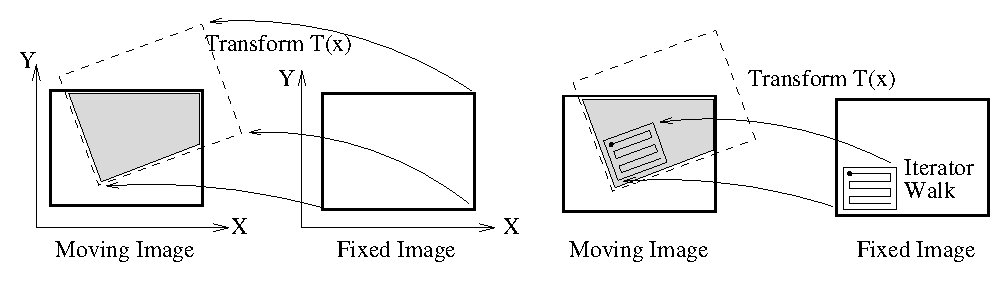
\includegraphics[width=\textwidth]{ImageOverlap.eps}
\itkcaption[Mapping moving image to fixed image in Registration]{ The moving
image is mapped into the fixed image space under some spatial
transformation. An iterator walks through the fixed image and its coordinates
are mapped onto the moving image.}
\label{fig:ImageOverlapIterator}
\end{figure}


\begin{floatingfigure}[rlp]{0.5\textwidth}
 \centering
 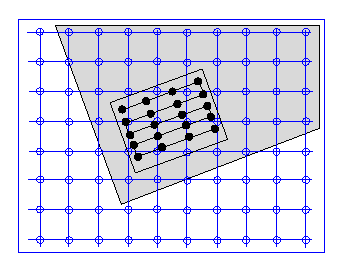
\includegraphics[width=7.5cm]{ImageOverlapInterpolator.eps}
 \caption[Need for interpolation in Registration]{Grid positions of the fixed
image map to non-grid positions of the moving
image.  \label{fig:ImageOverlapInterpolator}}
\end{floatingfigure}

In the registration process, the metric typically compares intensity values
in the fixed image against the corresponding values in the transformed moving
image. When a point is mapped from one space to another by a transform, it
will in general be mapped to a non-grid position. Therefore, interpolation is
required to evaluate the image intensity at the mapped position.

Figure \ref{fig:ImageOverlapIterator} (left) illustrates the mapping of the
fixed image space onto the moving image space. The transform maps points from
the fixed image coordinate system onto the moving image coordinate system. The
figure highlights the region of overlap between the two images after the
mapping. The right side illustrates how an iterator is used to walk through a
region of the fixed image. Each one of the iterator positions is mapped by the
transform onto the moving image space in order to find the homologous pixel.

Figure \ref{fig:ImageOverlapInterpolator} presents a detailed view of the
mapping from the fixed image to the moving image. In general, the grid
positions of the fixed image will not be mapped onto grid positions of the
moving image.  Interpolation is needed for estimating the intensity of the
moving image at these non-grid positions. The service is provided in ITK by
interpolator classes that can be plugged into the registration method.

\index{Nearest\-Neighbor\-Interpolate\-Image\-Function}
\index{Linear\-Interpolate\-Image\-Function}
\index{BSpline\-Interpolate\-Image\-Function}
\index{Windowed\-Sinc\-Interpolate\-Image\-Function}

The following interpolators are available:

\begin{itemize}
\item \doxygen{NearestNeighborInterpolateImageFunction}
\item \doxygen{LinearInterpolateImageFunction}
\item \doxygen{BSplineInterpolateImageFunction}
\item \doxygen{WindowedSincInterpolateImageFunction}
\end{itemize}

In the context of registration, the interpolation method affects the smoothness
of the optimization search space and the overall computation time. On the other
hand, interpolations are executed thousands of times in a single optimization
cycle. Hence, the user has to balance the simplicity of computation with the
smoothness of the optimization when selecting the interpolation scheme.

\index{itk::InterpolateImageFunction}
\index{itk::InterpolateImageFunction!SetInputImage()}
\index{itk::InterpolateImageFunction!Evaluate()}
\index{itk::InterpolateImageFunction!EvaluateAtContinuousIndex()}
\index{itk::InterpolateImageFunction!IsInsideBuffer()}

The basic input to an \doxygen{InterpolateImageFunction} is the image to
be interpolated. Once an image has been defined using \code{SetInputImage()},
a user can interpolate either at a point using \code{Evaluate()} or
an index using \code{EvaluateAtContinuousIndex()}.

Interpolators provide the method \code{IsInsideBuffer()} that tests whether a
particular image index or a physical point falls inside the spatial domain for
which image pixels exist.

\subsection{Nearest Neighbor Interpolation}
\label{sec:NearestNeighborInterpolation}
\index{itk::Nearest\-Neighbor\-Interpolate\-Image\-Function}
The \doxygen{NearestNeighborInterpolateImageFunction} simply uses the
intensity of the nearest grid position. That is, it assumes that the image
intensity is piecewise constant with jumps mid-way between grid positions.
This interpolation scheme is cheap as it does not require any floating point
computations.


\subsection{Linear Interpolation}
\label{sec:LinearInterpolation}
\index{itk::Linear\-Interpolate\-Image\-Function}

The \doxygen{LinearInterpolateImageFunction} assumes that intensity varies
linearly between grid positions. Unlike nearest neighbor interpolation, the
interpolated intensity is spatially continuous. However, the intensity
gradient will be discontinuous at grid positions.


\subsection{B-Spline Interpolation}
\label{sec:BSplineInterpolation}
\index{itk::BSpline\-Interpolate\-Image\-Function}

\begin{figure}
\center
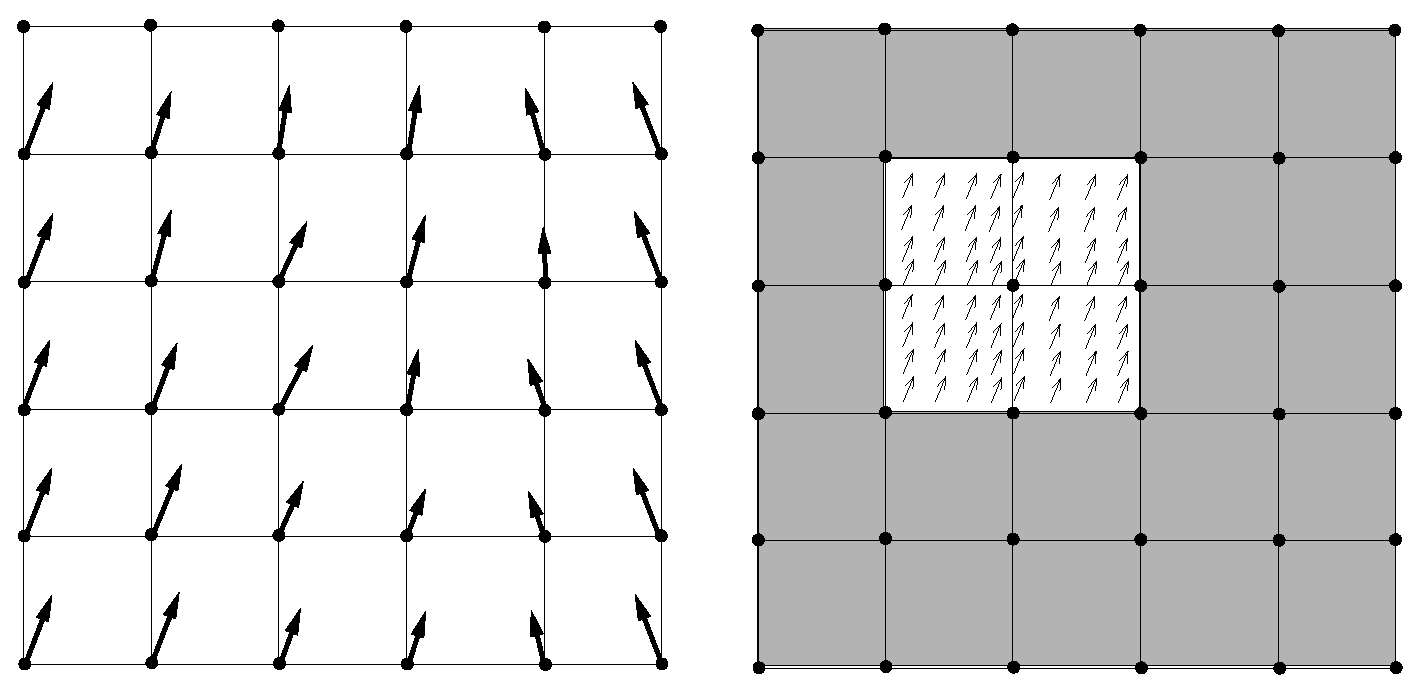
\includegraphics[width=0.9\textwidth]{BSplineInterpolation.eps}
\itkcaption[BSpline Interpolation Concepts]{The left side illustrates the
BSpline grid and the deformations that are known on those nodes. The right side
illustrates the region where interpolation is possible when the BSpline is of
cubic order. The small arrows represent deformation values that were
interpolated from the grid deformations shown on the left side of the diagram.}
\label{fig:BSplineInterpolation}
\end{figure}


The \doxygen{BSplineInterpolateImageFunction} represents the image intensity
using B-spline basis functions. When an input image is first connected to the
interpolator, B-spline coefficients are computed using recursive filtering
(assuming mirror boundary conditions). Intensity at a non-grid position is
computed by multiplying the B-spline coefficients with shifted B-spline kernels
within a small support region of the requested position.
Figure~\ref{fig:BSplineInterpolation} illustrates on the left how the
deformation values on the BSpline grid nodes are used for computing
interpolated deformations in the rest of space. Note for example that when a
cubic BSpline is used, the grid must have one extra node in one side of the
image and two extra nodes on the other side, this along every dimension.

Currently, this interpolator supports splines of order $0$ to $5$. Using a
spline of order $0$ is almost identical to nearest neighbor interpolation; a
spline of order $1$ is exactly identical to linear interpolation. For splines
of order greater than $1$, both the interpolated value and its derivative are
spatially continuous.

It is important to note that when using this scheme, the interpolated
value may lie outside the range of input image intensities. This is
especially important when handling unsigned data, as it is possible
that the interpolated value is negative.


\subsection{Windowed Sinc Interpolation}
\label{sec:WindowedSincInterpolation}
\index{itk::Windowed\-Sinc\-Interpolate\-Image\-Function}

The \doxygen{WindowedSincInterpolateImageFunction} is the best possible
interpolator for data that have been digitized in a discrete grid. This
interpolator has been developed based on Fourier Analysis considerations. It
is well known in signal processing that the process of sampling a spatial
function using a periodic discrete grid results in a replication of the
spectrum of that signal in the frequency domain.

The process of recovering the continuous signal from the discrete sampling is
equivalent to the removal of the replicated spectra in the frequency domain.
This can be done by multiplying the spectra with a box function that will set
to zero all the frequencies above the highest frequency in the original signal.
Multiplying the spectrum with a box function is equivalent to convolving the
spatial discrete signal with a sinc function

\begin{equation}
sinc(x) = \sin{(x)} / x
\end{equation}

The sinc function has infinite support, which of course in practice can not
really be implemented. Therefore, the sinc is usually truncated by multiplying
it with a Window function. The Windowed Sinc interpolator is the result of such an
operation.

This interpolator presents a series of trade-offs in its utilization. Probably
the most significant is that the larger the window, the more precise will be
the resulting interpolation. However, large windows will also result in long
computation times. Since the user can select the window size in this
interpolator, it is up to the user to determine how much interpolation quality
is required in her/his application and how much computation time can be
justified. For details on the signal processing theory behind this
interpolator, please refer to Meijering \emph{et.
al}~\cite{SignalReconstruction}.

The region of the image used for computing the interpolator is determined by
the window \emph{radius}. For example, in a $2D$ image where we want to
interpolate the value at position $(x,y)$ the following computation will be
performed.

\begin{equation}
I(x,y) =
\sum_{i = \lfloor x \rfloor + 1 - m}^{\lfloor x \rfloor + m}
\sum_{j = \lfloor y \rfloor + 1 - m}^{\lfloor y \rfloor + m}
I_{i,j} K(x-i) K(y-j)
\end{equation}

where $m$ is the \emph{radius} of the window. Typically, values such as 3 or 4
are reasonable for the window radius. The function kernel $K(t)$ is composed by
the $sinc$ function and one of the windows listed above.

\begin{equation}
K(t) = w(t) \textrm{sinc}(t) = w(t) \frac{\sin(\pi t)}{\pi t}
\end{equation}

Some of the windows that can be used with this interpolator are

Cosinus window
\begin{equation}
w(x) = cos ( \frac{\pi x}{2 m} )
\end{equation}


Hamming window
\begin{equation}
w(x) = 0.54 + 0.46 cos ( \frac{\pi x}{m} )
\end{equation}


Welch window
\begin{equation}
w(x) = 1 - ( \frac{x^2}{m^2} )
\end{equation}


Lancos window
\begin{equation}
w(x) = \textrm{sinc} ( \frac{x}{m} )
\end{equation}


Blackman window
\begin{equation}
w(x) = 0.42 + 0.5 cos(\frac{\pi x}{m}) + 0.08 cos(\frac{2 \pi x}{m})
\end{equation}


The window functions listed above are available inside the itk::Function
namespace. The conclusions of the referenced paper suggest to use the Welch,
Cosine, Kaiser, and Lancos windows for m = 4,5. These are based on error in
rotating medical images with respect to the linear interpolation method. In
some cases the results achieve a 20-fold improvement in accuracy.

This filter can be used in the same way you would use any
ImageInterpolationFunction. For instance, you can plug it into the
ResampleImageFilter class.  In order to instantiate the filter you must choose
several template parameters.

\small
\begin{minted}[baselinestretch=1,fontsize=\footnotesize,linenos=false,bgcolor=ltgray]{c++}
using InterpolatorType = WindowedSincInterpolateImageFunction<
           TInputImage, VRadius, TWindowFunction,
           TBoundaryCondition, TCoordRep >;

\end{minted}
\normalsize

\code{TInputImage} is the image type, as for any other interpolator.

\code{VRadius} is the radius of the kernel, i.e., the $m$ from the
formula above.

\code{TWindowFunction} is the window function object, which you can choose from
about five different functions defined in this header. The default is the
Hamming window, which is commonly used but not optimal according to the cited
paper.

\code{TBoundaryCondition} is the boundary condition class used to determine the
values of pixels that fall off the image boundary. This class has the same
meaning here as in the \doxygen{NeighborhoodIterator} classes.

\code{TCoordRep} is again standard for interpolating functions, and should be
float or double.


The WindowedSincInterpolateImageFunction is probably not the interpolator that
you want to use for performing registration. Its computation burden makes it
too expensive for this purpose. The best use of this interpolator is for the
final resampling of the image, once the transform has been found using
another less expensive interpolator in the registration process.

\fi

% the clearpage command helps to avoid orphans in the title of the next
% section.
\clearpage

\section{Metrics}
\label{sec:Metrics}
\ifitkFullVersion
%
%  This file is included by Registration.tex
%
%
%

\index{itk::Image\-To\-Image\-Metric}

In ITK, \doxygen{ImageToImageMetric} objects quantitatively measure how well
the transformed moving image fits the fixed image by comparing the gray-scale
intensity of the images. These metrics are very flexible and can work with any
transform or interpolation method and do not require reduction of the
gray-scale images to sparse extracted information such as edges.

The metric component is perhaps the most critical element of the registration
framework. The selection of which metric to use is highly dependent on the
registration problem to be solved. For example, some metrics have a large
capture range while others require initialization close to the optimal
position.  In addition, some metrics are only suitable for comparing images 
obtained from the same imaging modality, while others can handle 
inter-modality comparisons.
Unfortunately, there are no clear-cut rules as to how to choose a metric.

\index{itk::Image\-To\-Image\-Metric!GetValue()}
\index{itk::Image\-To\-Image\-Metric!GetDerivatives()}
\index{itk::Image\-To\-Image\-Metric!GetValueAndDerivatives()}

The basic inputs to a metric are: the fixed and moving images, a transform and
an interpolator. The method \code{GetValue()} can be used to evaluate the
quantitative criterion at the transform parameters specified in the argument.
Typically, the metric samples points within a defined region of the fixed
image.  For each point, the corresponding moving image position is computed
using the transform with the specified parameters, then the interpolator is
used to compute the moving image intensity at the mapped position. Details on
this mapping are illustrated in Figures \ref{fig:ImageOverlapIterator} and
\ref{fig:ImageOverlapInterpolator}. 

The metrics also support region based evaluation. The \code{SetFixedImageMask()} and 
\code{SetMovingImageMask()} methods may be used to restrict evaluation of the metric 
within a specified region. The masks may be of any type derived from \doxygen{SpatialObject}.

Besides the measure value, gradient-based optimization schemes also require
derivatives of the measure with respect to each transform parameter. The
methods \code{GetDerivatives()} and \code{GetValueAndDerivatives()} can be
used to obtain the gradient information.


The following is the list of metrics currently available in ITK:
\begin{itemize}
\item mean squares\\ \doxygen{MeanSquaresImageToImageMetric}
\item normalized correlation \\ \doxygen{NormalizedCorrelationImageToImageMetric}
\item mean reciprocal squared difference \\ \doxygen{MeanReciprocalSquareDifferenceImageToImageMetric} 
\item mutual information by Viola and Wells \\ \doxygen{MutualInformationImageToImageMetric}
\item mutual information by Mattes \\ \doxygen{MattesMutualInformationImageToImageMetric}
\item Kullback Liebler distance metric by Kullback and Liebler \\ \doxygen{KullbackLeiblerCompareHistogramImageToImageMetric}
\item Normalized mutual information \\ \doxygen{NormalizedMutualInformationHistogramImageToImageMetric}
\item Cardinality Match metric \\ \doxygen{MatchCardinalityImageToImageMetric}
\item Kappa Statistics metric\\ \doxygen{KappaStatisticImageToImageMetric}
\item Gradient Difference metric \\ \doxygen{GradientDifferenceImageToImageMetric}
\end{itemize}

In the following sections, we describe each metric type in detail. 
For ease of notation, we will refer to the fixed image $f(\bf{X})$ 
and transformed moving image $(m \circ T(\bf{X}))$ as images $A$ and $B$.

\subsection{Mean Squares Metric}
\label{sec:MeanSquaresMetric}
\index{itk::Mean\-Squares\-Image\-To\-Image\-Metric}

The \doxygen{MeanSquaresImageToImageMetric} computes the mean squared
pixel-wise difference in intensity between image $A$ and $B$ over a user
defined region:

\begin{equation}
MS(A,B) = \frac{1}{N} \sum_{i=1}^N \left( A_i - B_i \right)^2
\end{equation}
\begin{center}
$A_i$ is the i-th pixel of Image A\\ 
$B_i$ is the i-th pixel of Image B\\
$N$ is the number of pixels considered
\end{center}

The optimal value of the metric is zero. Poor matches between images $A$ and
$B$ result in large values of the metric. This metric is simple to compute and
has a relatively large capture radius.

This metric relies on the assumption that intensity representing the same
homologous point must be the same in both images. Hence, its use is restricted
to images of the same modality. Additionally, any linear changes in the
intensity result in a poor match value.

\subsubsection{Exploring a Metric}
\label{sec:ExploringAMetric}

Getting familiar with the characteristics of the Metric as a cost function is
fundamental in order to find the best way of seting up an optimization process
that will use this metric for solving a registration problem. 

\ifitkFullVersion
\input{MeanSquaresImageMetric1.tex}
\fi


\subsection{Normalized Correlation Metric}
\label{sec:NormalizedCorrelationMetric}
\index{itk::Normalized\-Correlation\-Image\-To\-Image\-Metric}

The \doxygen{NormalizedCorrelationImageToImageMetric} computes pixel-wise
cross-correlation and normalizes it by the square root of the autocorrelation
of the images:

\begin{equation}
NC(A,B) = -1 \times \frac{ \sum_{i=1}^N \left( A_i \cdot B_i \right) }
        { \sqrt { \sum_{i=1}^N A_i^2  \cdot \sum_{i=1}^N B_i^2 } }
\end{equation}
\begin{center}
$A_i$ is the i-th pixel of Image A\\ 
$B_i$ is the i-th pixel of Image B\\
$N$ is the number of pixels considered
\end{center}

Note the $-1$ factor in the metric computation. This factor is used to make the
metric be optimal when its minimum is reached.  The optimal value of the metric
is then minus one. Misalignment between the images results in small measure
values.  The use of this metric is limited to images obtained using the same
imaging modality.  The metric is insensitive to multiplicative factors between
the two images.  This metric produces a cost function with sharp peaks and well
defined minima.  On the other hand, it has a relatively small capture radius.

\subsection{Mean Reciprocal Square Differences}
\label{sec:MeanReciprocalSquareDifferenceMetric}
\index{itk::Mean\-Reciprocal\-Square\-Difference\-Image\-To\-Image\-Metric}

The \doxygen{MeanReciprocalSquareDifferenceImageToImageMetric} computes
pixel-wise differences and adds them after passing them through a bell-shaped
function $\frac{1}{1+x^2}$:

\begin{equation}
PI(A,B) =  \sum_{i=1}^N \frac{ 1 }{ 1 + \frac{ \left( A_i - B_i \right) ^ 2}{ \lambda^2 }  }
\end{equation}
\begin{center}
$A_i$ is the i-th pixel of Image A \\
$B_i$ is the i-th pixel of Image B \\
$N$ is the number of pixels considered \\
$\lambda$ controls the capture radius
\end{center}

The optimal value is $N$ and poor matches results in small measure values.
The characteristics of this metric have been studied by Penney and Holden
\cite{Holden1999}\cite{Penney1998}

This image metric has the advantage of producing poor values when few pixels
are considered.  This makes it consistent when its computation is subject to
the size of the overlap region between the images. The capture radius of the
metric can be regulated with the parameter $\lambda$.  The profile of this
metric is very peaky. The sharp peaks of the metric help to measure spatial
misalignment with high precision. Note that the notion of capture radius is
used here in terms of the intensity domain, not the spatial domain. In that
regard, $\lambda$ should be given in intensity units and be associated with
the differences in intensity that will make drop the metric by $50\%$.

The metric is limited to images of the same image modality.  The
fact that its derivative is large at the central peak is a problem for some
optimizers that rely on the derivative to decrease as the extrema are
reached.  This metric is also sensitive to linear changes in intensity.


\subsection{Mutual Information Metric}
\label{sec:MutualInformationMetric}

The \doxygen{MutualInformationImageToImageMetric} computes the mutual
information between image $A$ and image $B$.  Mutual information (MI)
measures how much information one random variable (image intensity in one
image) tells about another random variable (image intensity in the other
image). The major advantage of using MI is that the actual form of the
dependency does not have to be specified.  Therefore, complex mapping between
two images can be modeled.  This flexibility makes MI well suited as a
criterion of multi-modality registration~\cite{Pluim2003}.

Mutual information is defined in terms of entropy. Let
\begin{equation}
H(A) = - \int p_A(a) \log p_A(a)\, da
\end{equation}
be the entropy of random variable $A$, $H(B)$ the entropy of 
random variable $B$ and 
\begin{equation}
H(A,B) = \int p_{AB}(a,b) \log p_{AB}(a,b)\,da\,db
\end{equation}
be the joint entropy of $A$ and $B$. If $A$ and $B$ are independent, then
\begin{equation}
p_{AB}(a,b) = p_A(a) p_B(b)
\end{equation}
and
\begin{equation}
H(A,B) = H(A) + H(B).
\end{equation}
However, if there is any dependency, then
\begin{equation}
H(A,B)<H(A)+H(B).
\end{equation}
The difference is called Mutual Information : \( I(A,B) \)
\begin{equation}
I(A,B)=H(A)+H(B)-H(A,B)
\end{equation}

\subsubsection{Parzen Windowing}

\itkpiccaption[Parzen Windowing in Mutual Information]{
In Parzen windowing, a continuous density function is constructed by
superimposing kernel functions (Gaussian function in this case) centered on the
intensity samples obtained from the image.\label{fig:ParzenWindowing}}
\parpic(0.5\textwidth,5.5cm)[r]{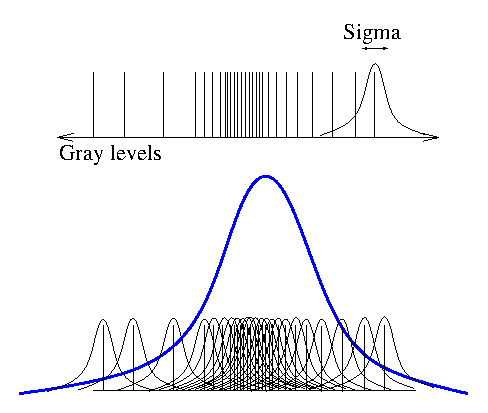
\includegraphics[width=0.48\textwidth]{ParzenWindowing13.eps}}

In a typical registration problem, direct access to the marginal 
and joint probability densities is not available and hence the
densities must be estimated from the image data. Parzen windows 
(also known as kernel density estimators) can be used for this purpose.
In this scheme, the densities are constructed by taking intensity 
samples $S$ from the image and super-positioning kernel functions 
$K(\cdot)$ centered on the elements of $S$ as illustrated in
Figure \ref{fig:ParzenWindowing}:

A variety of functions can be used as the smoothing kernel with the
requirement that they are smooth, symmetric, have zero mean and
integrate to one. For example, boxcar, Gaussian and B-spline functions are
suitable candidates.  A smoothing parameter is used to scale the kernel
function.  The larger the smoothing parameter, the wider the kernel function
used and hence the smoother the density estimate. If the parameter is too
large, features such as modes in the density will get smoothed out.  On the
other hand, if the smoothing parameter is too small, the resulting density
may be too noisy. The estimation is given by the following equation.

\begin{equation}
p(a) \approx P^{*}(a) = \frac{1}{N} \sum_{s_j \in S} K\left(a - s_j\right)
\end{equation}

Choosing the optimal smoothing parameter is a difficult research problem and
beyond the scope of this software guide.  Typically, the optimal value of the
smoothing parameter will depend on the data and the number of samples used.

\subsubsection{Viola and Wells Implementation}

The Insight Toolkit has two mutual information metric implementations. The
first is \doxygen{MutualInformationImageToImageMetric} and follows the method
specified by Viola and Wells in \cite{Viola1997}.

\index{itk::Mutual\-Information\-Image\-To\-Image\-Metric}

In this implementation, two separate intensity samples $S$ and $R$ are drawn
from the image: the first to compute the density, and the second to approximate
the entropy as a sample mean:
\begin{equation}
H(A) = \frac{1}{N} \sum_{r_j \in R} \log P^{*}(r_j).
\end{equation}
Gaussian density is used as a smoothing kernel, where the standard deviation
$\sigma$ acts as the smoothing parameter.

\index{itk::Mutual\-Information\-Image\-To\-Image\-Metric!SetNumberOfSpatialSamples()}

The number of spatial samples used for computation is defined using
the \code{SetNumberOfSpatialSamples()} method. Typical values range from 50 to 100.
Note that computation involves an $N \times N$ loop and hence, the computation
burden becomes very expensive when a large number of samples is used.

\index{itk::Mutual\-Information\-Image\-To\-Image\-Metric!SetFixedImageStandardDeviation()}
\index{itk::Mutual\-Information\-Image\-To\-Image\-Metric!SetMovingImageStandardDeviation()}
The quality of the density estimates depends on the choice of the standard
deviation of the Gaussian kernel. The optimal choice will depend on the
content of the images.  In our experience with the toolkit, we have found
that a standard deviation of 0.4 works well for images that have been
normalized to have a mean of zero and standard deviation of 1.0. The standard
deviation of the fixed image and moving image kernel can be set separately
using methods
\code{SetFixedImageStandardDeviation()} and \code{SetMovingImageStandardDeviation()}.

\subsubsection{Mattes et al. Implementation}
The second form of mutual information metric available in ITK follows the
method specified by Mattes et al. in \cite{Mattes2001} and is implemented by
the \doxygen{MattesMutualInformationImageToImageMetric} class.

\index{itk::Mattes\-Mutual\-Information\-Image\-To\-Image\-Metric}
In this implementation, only one set of intensity samples is drawn from the
image.  Using this set, the marginal and joint probability density function
(PDF) is evaluated at discrete positions or bins uniformly spread within the
dynamic range of the images. Entropy values are then computed by summing over
the bins.

\index{itk::Mattes\-Mutual\-Information\-Image\-To\-Image\-Metric!SetNumberOfSpatialSamples()}
\index{itk::Mattes\-Mutual\-Information\-Image\-To\-Image\-Metric!SetNumberOfHistogramBins()}

The number of spatial samples used is set using method 
\code{SetNumberOfSpatialSamples()}. The number of bins used to compute
the entropy values is set via \code{SetNumberOfHistogramBins()}.

Since the fixed image PDF does not contribute to the metric derivatives, it
does not need to be smooth. Hence, a zero order (boxcar) B-spline kernel is
used for computing the PDF. On the other hand, to ensure smoothness, a third
order B-spline kernel is used to compute the moving image intensity PDF. The
advantage of using a B-spline kernel over a Gaussian kernel is that the
B-spline kernel has a finite support region. This is computationally
attractive, as each intensity sample only affects a small number of bins and
hence does not require a $N \times N$ loop to compute the metric value.

During the PDF calculations, the image intensity values are linearly scaled
to have a minimum of zero and maximum of one. This rescaling means that a
fixed B-spline kernel bandwidth of one can be used to handle image data with
arbitrary magnitude and dynamic range.


\subsection{Kullback-Leibler distance metric}
Another information based metric is the \doxygen{KullbackLeiblerCompareHistogramImageToImageMetric} metric. Kullback-Leibler distance measures the relative entropy between two discrete 
probability distributions. The distributions are obtained from the histograms of the two 
input images, $A$ and $B$. 

The Kullback-Liebler distance between two histograms is given by
\begin{equation}
KL(A,B) =  \sum_i^N p_A(i) \times \log \frac{ p_A(i) }{p_B(i) }
\end{equation}

The distance is always non-negative and is zero only if the two distributions 
are the same. Note that the distance is not symmetric. In other 
words, $KL(A,B) \neq KL(B,A)$. Nevertheless, if the distributions are not too dissimilar, 
the difference betwween $KL(A,B)$ and $KL(B,A)$ is small.

The implementation in ITK is based on \cite{Chung2002}

\subsection{Normalized Mutual Information Metric}
Given two images, $A$ and $B$, the normalized mutual information may be computed as 
\begin{equation}
NMI(A,B) = 1 + \frac{I(A,B)}{H(A,B)} = \frac{H(A) + H(B)}{H(A,B)}
\end{equation}
where the entropy of the images, $H(A)$, $H(B)$, the mutual 
inoformation, $I(A,B)$ and the joint entropy $H(A,B)$ are computed as mentioned 
in \ref{sec:MutualInformationMetric}. Details of the implementation may be found in 
the \cite{Hajnal2001}.

\subsection{Cardinality Match Metric}
\index{itk::Match\-Cardinality\-Image\-To\-Image\-Metric}
The \doxygen{MatchCardinalityImageToImageMetric} computes cardinality of the set of pixels 
that match exactly between the moving and fixed images. In other words, it computes the 
number of pixel matches and mismatches between the two images. The match is designed for 
label maps. All pixel mismatches are considered equal whether they are between label 1 
and label 2 or between label 1 and label 500. In other words, the magnitude of an 
individual label mismatch is not relevant, or the occurence of a label mismatch 
is important. 

The spatial correspondance between the fixed and moving images is established using 
a \doxygen{Transform} using the \code{SetTransform()} method and an interpolator 
using \code{SetInterpolator()}. Given that we are matching pixels with labels, 
it is advisable to use Nearest Neighbor interpolation.

\subsection{Kappa Statistics Metric}
\index{itk::Kappa\-Statistic\-Image\-To\-Image\-Metric}
The \doxygen{KappaStatisticImageToImageMetric} computes spatial intersection of 
two binary images. The metric here is designed for matching pixels in two images 
with the same exact value, which may be set using \code{SetForegroundValue()}. 
Given two images $A$ and $B$, the $\kappa$ coefficient is computed as
 
\begin{equation}
\kappa = \frac{|A| \cap |B|}{|A| + |B|}
\end{equation}

This computes the fraction of area in the two images that is common to both 
the images. In the computation of the metric, only foreground pixels are considered.

\subsection{Gradient Difference Metric}
\index{it::Gradient\-Difference\-Image\-To\-Image\-Metric}
This \doxygen{GradientDifferenceImageToImageMetric} metric evaluates the 
difference in the derivatives of the moving and fixed images. and adds 
them after passing them through a function $\frac{1}{1+x}$.



\fi

% the clearpage command helps to avoid orphans in the title of the next
% section.
\clearpage

\section{Optimizers}
\label{sec:Optimizers}
\ifitkFullVersion

\index{itk::Optimizer|textbf}
\index{itk::SingleValuedNonLinearOptimizer|textbf}


\begin{figure}
\center
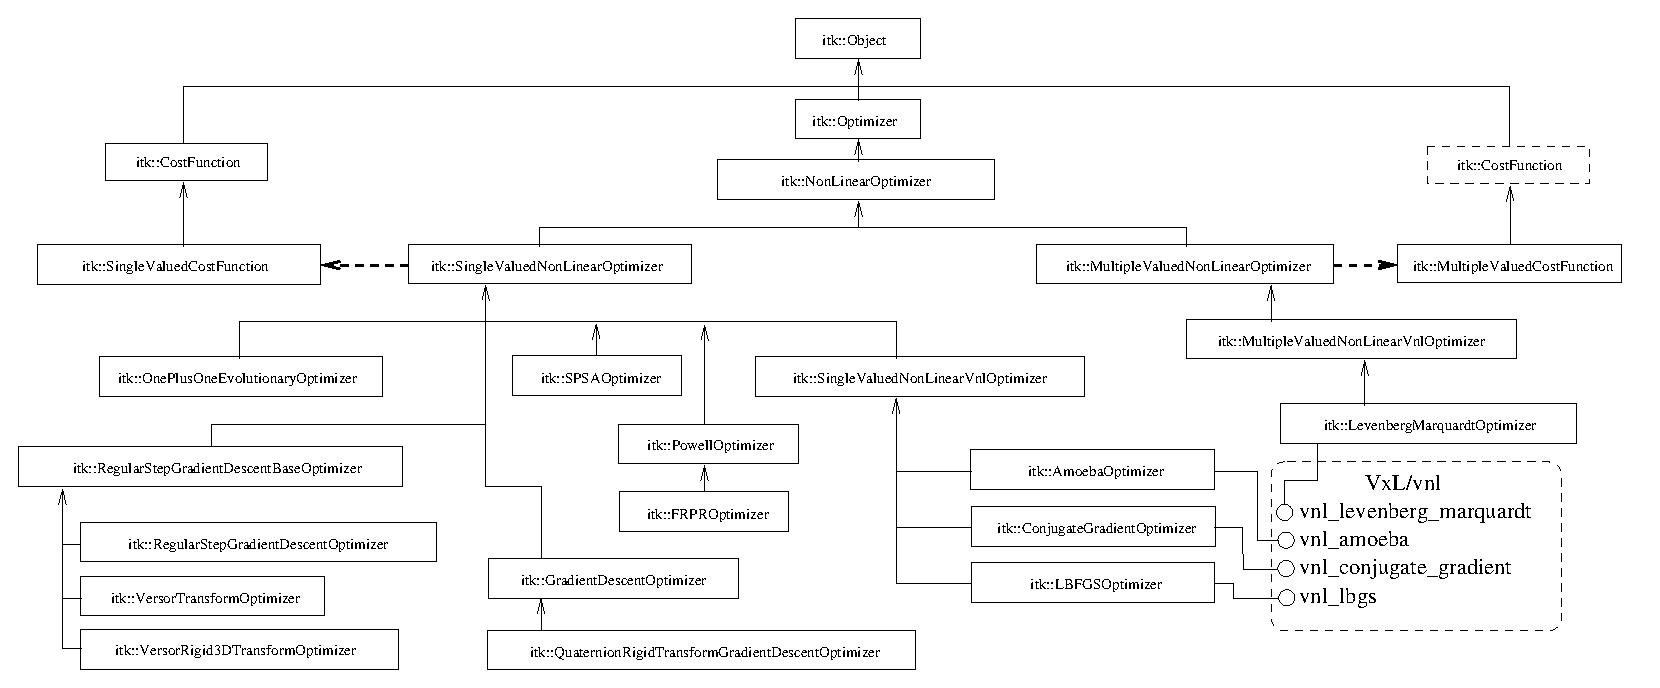
\includegraphics[width=16cm]{OptimizersHierarchy.eps}
\itkcaption{Class diagram of the Optimizers hierarchy.}
\label{fig:OptimizersHierarchy}
\end{figure}

Optimization algorithms are encapsulated as \code{itk::Optimizer} objects
within ITK. Optimizers are generic and can be used for applications other than
registration.  Within the registration framework,
\code{itk::SingleValuedNonLinearOptimizer} are used to optimize the metric
criterion with respect to the transform parameters.

\index{itk::Optimizer!SetInitialPosition()}
\index{itk::Optimizer!StartOptimization()}
\index{itk::Optimizer!GetCurrentPosition()}

The basic input to an optimizer is a cost function object. In the context
of registration, \code{itk::ImageToImageMetric} provide this functionality.
The initial parameters are set using \code{SetInitialPosition()} and
the optimization algorithm is invoked by \code{StartOptimization()}.
Once the optimization has finished, the final parameters can be obtained
using \code{GetCurrentPosition()}.

\index{itk::Optimizer!SetScales()}
Some optimizers also allows rescaling of the individual parameters. This
is convenient for normalizing parameters spaces where some parameters
have different dynamic ranges. For example, the first parameter of
\code{Euler2DTransform} represent an angle while the last two parameters
the translation. A unit change in angle has a much greater impact on
an image than a unit change in translation. This difference in scale appears
as long narrow valleys in the search space making the optimization problem
diffcult. Rescaling the translation parameters can help to fix this problem.
Scales are represented as \code{Array} of doubles and set defined using
\code{SetScales()}.

The types of \code{itk::SingleValuedNonLinearOptimizer} currently available
in ITK are:

\index{itk::AmoebOptimizer|textbf}
\index{itk::ConjugateGradientOptimizer|textbf}
\index{itk::GradientDescentOptimizer|textbf}
\index{itk::QuaternionRigidTransformGradientDescentOptimizer|textbf}
\index{itk::LBFGSOptimizer|textbf}
\index{itk::OnePlusOneEvolutionaryOptimizer|textbf}
\index{itk::RegularStepGradientDescentOptimizer|textbf}
\index{itk::VersorTransformOptimizer|textbf}
\index{itk::LevenbergMarquardtOptimizer|textbf}

\begin{itemize}

\item \textbf{Amoeba}: Nelder-Meade downhill simplex.  This optimizer is
actually implemented in the \code{VxL/vnl} numerics toolkit.  The ITK class
\code{itk::AmoebaOptimizer} is merely an adaptor class.

\item \textbf{Conjugate Gradient}: Fletcher-Reeves form 
of conjugate gradient with or without preconditioning. Also an adaptor to an
optimizer in \code{vnl}.

\item \textbf{Gradient Descent}: Advance parameters in the direction of the
gradient where the step size is governed by a learning rate. 

\item \textbf{Quaternion Rigid Transform Gradient Descent}: 
A specialized version of \code{GradientDescentOptimizer} for
\code{QuaternionRigidTransform} parameters, where the parameters representing
the quaternion is normalize to a magnitude to one at each iteration to
represent a pure rotation.

\item \textbf{LBFGS}: Limited memory Broyden, Fletcher, Goldfarb
and Shannon minmization. It is an adaptor to an optimizer in \code{vnl}.

\item \textbf{One Plus One Evolutionary}: Strategy that simulates the
biological evolution of a set of samples in the search space. This optimizer
is mainly used in the process of bias correction for MRI images.

\item \textbf{Regular Step Gradient Descent}: Advance parameters in the
direction of the gradient where a bipartition scheme is used to compute
the step size. 

\item \textbf{Versor Transform Optimizer}: A specialized version of
\code{RegularStepGradientDescentOptimizer} for \code{VersorTransform}
parameters  where the current rotation is composed with the gradient rotation
to produce the new rotation vector. It follows the definition of versor
gradients defined by Hamilton~\cite{Hamilton1866}.

\end{itemize}

A parallel hierarchy exists for optimizing multiple-valued cost functions. The
base optimizer in this branch of the hierarchy is the
\code{itk::MultipleValuedNonLinearOptimizer} whose only current derived class
is:

\begin{itemize}

\item \textbf{Levenberg Marquardt}: Non-linear least squares minimization.
Adapted to an optimizer in \code{vnl}.

\end{itemize}


Figure \ref{fig:OptimizersHierarchy} illustrates the full class hierarchy of
optimizers in ITK. Optimizers in the lower right corner are adaptors classes to
optimizers existing in the \code{VxL/vnl} numerics toolkit. The optimizers
interact with the \code{itk::CostFunction} class. In the registration framework
this cost function is reimplemented in the form of \code{itk::ImageToImageMetric}.






\fi



\subsection{Registration using Match Cardinality metric}
\label{sec:RegistrationMatchCardinality}
\ifitkFullVersion
\input{ImageRegistration10.tex}
\fi


\subsection{Registration using the One plus One Evolutionary Optimizer}
\label{sec:RegistrationOnePlusOne}
\ifitkFullVersion
\input{ImageRegistration11.tex}
\fi



\subsection{Registration using masks constructed with Spatial objects}
\label{sec:RegistrationSpatialObjects}
\ifitkFullVersion
\input{ImageRegistration12.tex}
\fi



\subsection{Rigid registrations incorporating prior knowledge}
\label{sec:RegistrationCentered2DTransform}
\ifitkFullVersion
\input{ImageRegistration13.tex}
\fi
% the clearpage command helps to avoid orphans in the title of the next
% section.
\clearpage

\section{Image Pyramids}
\label{sec:ImagePyramids}
\ifitkFullVersion

\index{itk::Multi\-Resolution\-Pyramid\-Image\-Filter}

In ITK, the \doxygen{MultiResolutionPyramidImageFilter} can be used to create
a sequence of reduced resolution images from the input image.  The
down-sampling is performed according to a user defined multi-resolution
schedule. The schedule is specified as an \doxygen{Array2D} of integers,
containing shrink factors for each multi-resolution level (rows) for each
dimension (columns). For example,

\small
\begin{verbatim}
8 4 4
4 4 2
\end{verbatim}
\normalsize

is a schedule for a three dimensional image for two multi-resolution levels.
In the first (coarsest) level, the image is reduced by a factor of 8
in the column dimension, factor of 4 in the row dimension and a factor
of 4 in the slice dimension. In the second level, the image reduced
by a factor of 4 in the column dimension, 4 in the row dimension and
2 in the slice dimension.

\index{itk::Multi\-Resolution\-Pyramid\-Image\-Filter!SetNumberOfLevels()}

The method \code{SetNumberOfLevels()} is used to set the number of
resolution levels in the pyramid. This method will allocate memory
for the schedule and generate a default table with the starting
(coarsest) shrink factors for all dimensions set to $2^(M-1)$,
where $M$ is the number of levels. All factors are halved for
all subsequent levels. For example, if we set the number of levels
to 4, the default schedule is then:

\small
\begin{verbatim}
8 8 8
4 4 4
2 2 2
1 1 1
\end{verbatim}
\normalsize

\index{itk::Multi\-Resolution\-Pyramid\-Image\-Filter!GetSchedule()}
\index{itk::Multi\-Resolution\-Pyramid\-Image\-Filter!SetSchedule()}
\index{itk::Multi\-Resolution\-Pyramid\-Image\-Filter!SetStartingShrinkFactors()}

The user can get a copy of the schedule using method \code{GetSchedule()},
make modifications, and reset it using method \code{SetSchedule()}.
Alternatively, a user can create a default table by specifying the
starting (coarsest) shrink factors using the method
\code{SetStartingShrinkFactors()}. The factors for the subsequent
levels are generated by halving the factor or setting it to one,
depending on which is larger. For example, for a 4 level pyramid
and starting factors of 8, 8 and 4, the generated schedule would be:

\small
\begin{verbatim}
8 8 4
4 4 2
2 2 1
1 1 1
\end{verbatim}
\normalsize

When this filter is triggered by \code{Update()}, $M$ outputs are produced
where the $m$-th output corresponds to the $m$-th level of the pyramid.
To generate these images, Gaussian smoothing is first performed using a
\doxygen{DiscreteGaussianImageFilter} with the variance set to $(s/2)^2$,
where $s$ is the shrink factor. The smoothed images are then sub-sampled using
a \doxygen{ShrinkImageFilter}.

\fi


% the clearpage command helps to avoid orphans in the title of the next
% section.
\clearpage

\section{Deformable Registration}
\label{sec:DeformableRegistration}
\ifitkFullVersion
%%%%%%%%%%%%%%%%%%%%%%%%%%%%%%%%%%%%%%%%%%%%%%%%%%%%%%%%%%%%%%%
%
%
%   This file is included in Registration.tex
%
%   Labels and section entries are defined in that file.
%
%
%
%%%%%%%%%%%%%%%%%%%%%%%%%%%%%%%%%%%%%%%%%%%%%%%%%%%%%%%%%%%%%%%


\subsection{FEM-Based Image Registration}
\label{sec:FEMBasedImageRegistration}

\begin{figure}
\centering
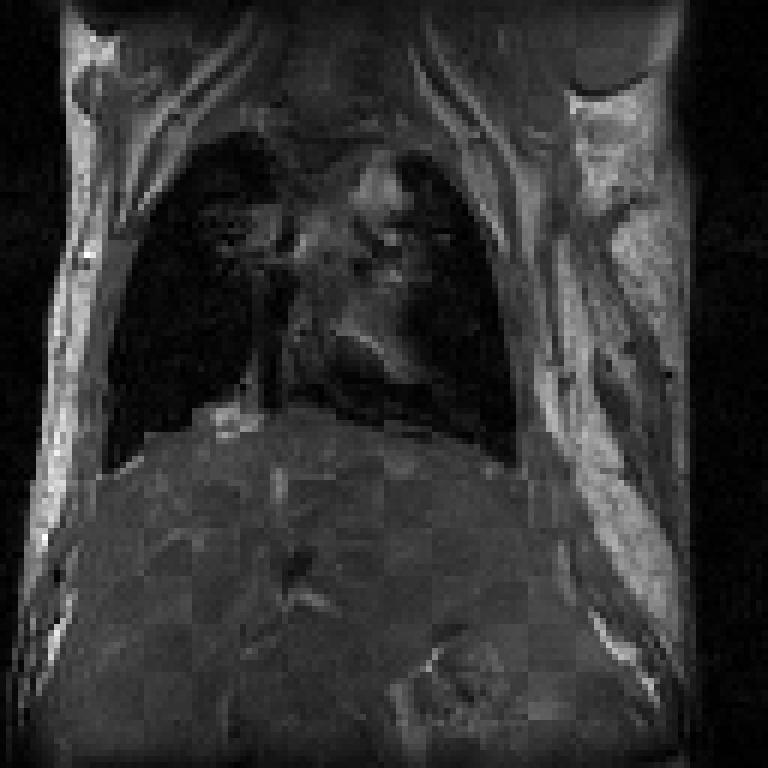
\includegraphics[width=0.44\textwidth]{DeformableRegistration1CheckerboardBefore.eps}
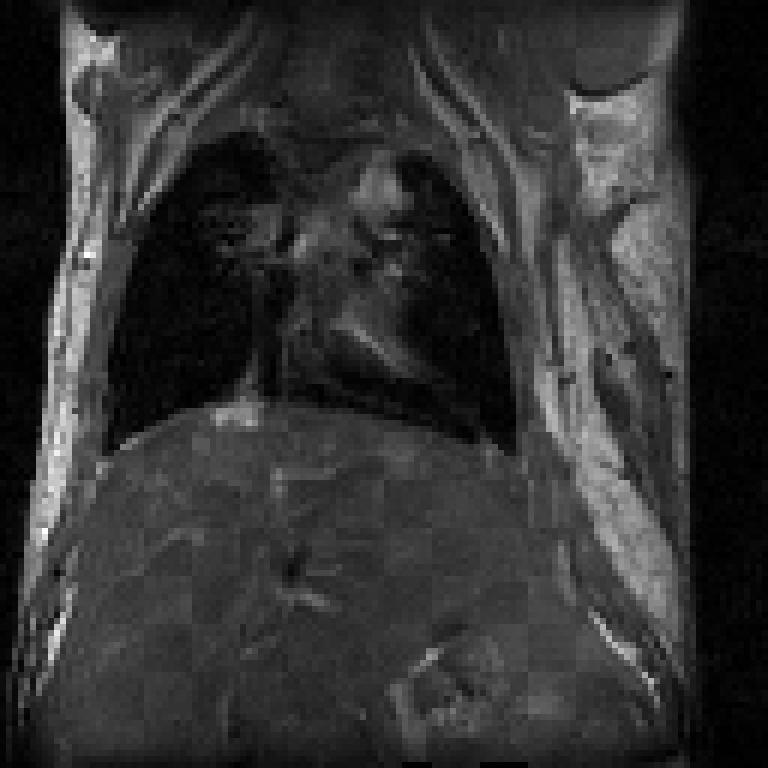
\includegraphics[width=0.44\textwidth]{DeformableRegistration1CheckerboardAfter.eps}
\itkcaption[FEM-based deformable registration results]{Checkerboard comparisons
before and after FEM-based deformable registration.}
\label{fig:DeformableRegistration1Output}
\end{figure}

\input{DeformableRegistration1.tex}

Figure \ref{fig:DeformableRegistration1Output} presents the results of
the FEM-based deformable registration applied to two time-separated
slices of a living rat dataset.  Checkerboard comparisons of the two
images are shown before registration (left) and after registration
(right).  Both images were acquired from the same living rat, the
first after inspiration of air into the lungs and the second after
exhalation.  Deformation occurs due to the relaxation of the diaphragm
and the intercostal muscles, both of which exert force on the lung tissue
and cause air to be expelled.

The following is a documented sample parameter file that can be used with this
deformable registration example.  This example demonstrates the setup of a
basic registration problem that does not use multi-resolution strategies.  As a
result, only one value for the parameters between \texttt{(\# of pixels per
element)} and \texttt{(maximum iterations)} is necessary.  In order to use a
multi-resolution strategy, you would have to specify values for those
parameters at each level of the pyramid.

\small
\verbatiminput{FiniteElementRegistrationParameters1.txt}
\normalsize

\subsection{BSplines Image Registration}
\label{sec:BSplinesImageRegistration}
\input{DeformableRegistration4.tex}


\subsection{Level Set Motion for Deformable Registration}
\label{sec:LevelSetMotionForDeformableRegistration}
\input{DeformableRegistration5.tex}


\subsection{BSplines Multi-Grid Image Registration}
\label{sec:BSplinesMultiGridImageRegistration}
\input{DeformableRegistration6.tex}


\subsection{BSplines Multi-Grid Image Registration in 3D}
\label{sec:BSplinesMultiGridImageRegistrationIn3D}
\input{DeformableRegistration7.tex}


\subsection{Image Warping with Kernel Splines}
\label{sec:ImageWarpingWithKernelSplines}
\input{LandmarkWarping2.tex}


\subsection{Image Warping with BSplines}
\label{sec:ImageWarpingWithBSplines}
\input{BSplineWarping1.tex}

\fi

% the clearpage command helps to avoid orphans in the title of the next
% section.
\clearpage

\section{Demons Deformable Registration}
\label{sec:DemonsDeformableRegistration}
\ifitkFullVersion
%%%%%%%%%%%%%%%%%%%%%%%%%%%%%%%%%%%%%%%%%%%%%%%%%%%%%%%%%%%%%%%
%
%
%   This file is included in Registration.tex
%
%   Lablels and section entries are defined in that file.
%
%
%
%%%%%%%%%%%%%%%%%%%%%%%%%%%%%%%%%%%%%%%%%%%%%%%%%%%%%%%%%%%%%%%

For the problem of intra-modality deformable registration, the Insight
Toolkit provides an implementation of Thirion's ``demons'' algorithm
\cite{Thirion1995b,Thirion1998}. 
In this implementation, each image is viewed as a set of iso-intensity
contours.  The main idea is that a regular grid of forces deform an image by
pushing the contours in the normal direction.  The orientation and magnitude
of the displacement is derived from the instantaneous optical flow equation:

\begin{equation}
\bf{D}(\bf{X}) \cdot \nabla f(\bf{X}) = - \left(m(\bf{X}) - f(\bf{X}) \right)
\label{eqn:OpticalFlow}
\end{equation}

In the above equation, $f(\bf{X})$ is the fixed image, $m(\bf{X})$
is the moving image to be registered, and $\bf{D}(\bf{X})$ is the displacement 
or optical flow between the images. It is well known in optical flow
literature that Equation \ref{eqn:OpticalFlow} is insufficient to specify 
$\bf{D}(\bf{X})$ locally and is usually determined using some form of
regularization. For registration, the projection of the vector on the
direction of the intensity gradient is used:

\begin{equation}
\bf{D}(\bf{X}) = - \frac
{\left(  m(\bf{X}) - f(\bf{X}) \right) \nabla f(\bf{X})}
{\left\|  \nabla f \right\|^2 } 
\end{equation}

However, this equation becomes unstable for small values of the image gradient,
resulting in large displacement values. To overcome this problem, Thirion
re-normalizes the equation such that:

\begin{equation}
\bf{D}(\bf{X}) = - \frac
{\left(  m(\bf{X}) - f(\bf{X}) \right) \nabla f(\bf{X})}
{\left\|  \nabla f \right\|^2 + \left(  m(\bf{X}) - f(\bf{X}) \right)^2 / K } 
\label{eqn:DemonsDisplacement}
\end{equation}

Where $K$ is a normalization factor that accounts for the units imbalance
between intensities and gradients. This factor is computed as the mean squared
value of the pixel spacings. The inclusion of $K$ make the force computation to
be invariant to the pixel scaling of the images.

Starting with an initial deformatin field $\bf{D}^{0}(\bf{X})$, the demons
algorithm iteratively updates the field using Equation
\ref{eqn:DemonsDisplacement} such that the field at the $N$-th iteration is
given by:

\begin{equation}
\bf{D}^{N}(\bf{X}) = \bf{D}^{N-1}(\bf{X}) - \frac
{\left(  m(\bf{X}+ \bf{D}^{N-1}(\bf{X})) 
- f(\bf{X}) \right) \nabla f(\bf{X})}
{\left\|  \nabla f \right\|^2 + \left(  
m(\bf{X}+ \bf{D}^{N-1}(\bf{X}) )
 - f(\bf{X}) \right)^2 } 
\label{eqn:DemonsUpdateEquation}
\end{equation}

Reconstruction of the deformation field is an ill-posed problem where
matching the fixed and moving images has many solutions. For example, since
each image pixel is free to move independently, it is possible that all
pixels of one particular value in $m(\bf{X})$ could map to a single image
pixel in $f(\bf{X})$ of the same value. The resulting deformation field may
be unrealistic for real-world applications. An option to solve for the field
uniquely is to enforce an elastic-like behavior, smoothing the deformation
field with a Gaussian filter between iterations.

In ITK, the demons algorithm is implemented as part of the finite difference
solver (FDS) framework and its use is demonstrated in the following example.

\input{DeformableRegistration2.tex} 

A variant of the force computation is also implemented in which the gradient of
the deformed moving image is also involved. This provides a level of symmetry
in the force calculation during one iteration of the PDE update. The equation
used in this case is

\begin{equation}
\bf{D}(\bf{X}) = - \frac
{2 \left(  m(\bf{X}) - f(\bf{X}) \right) \left(  \nabla f(\bf{X}) +  \nabla g(\bf{X}) \right) }
{\left\|  \nabla f + \nabla g \right\|^2 + \left(  m(\bf{X}) - f(\bf{X}) \right)^2 / K } 
\label{eqn:DemonsDisplacement}
\end{equation}

The following example illustrates the use of this defomable registration
method.

\input{DeformableRegistration3.tex} 




\fi

\section{Visualizing Deformation fields}
\label{sec:VisualizingDeformationFields}
\ifitkFullVersion
%%%%%%%%%%%%%%%%%%%%%%%%%%%%%%%%%%%%%%%%%%%%%%%%%%%%%%%%%%%%%%%
%
%
%   This file is included in Registration.tex
%
%   Lablels and section entries are defined in that file.
%
%
%
%%%%%%%%%%%%%%%%%%%%%%%%%%%%%%%%%%%%%%%%%%%%%%%%%%%%%%%%%%%%%%
Vector deformation fields may be visualized using Paraview.
Paraview \cite{ParaviewBook} is an open-source, multi-platform visualization application and uses the Visualization Toolkit as the data processing and rendering engine and has a user interface written using a unique blend of Tcl/Tk and C++. You may download it from http://paraview.org.

\subsection{Visualizing 2D deformation fields}
Let us visualize the deformation field obtained from Demons Registration algorithm generated from Insight/Examples/Registration/DeformableRegistration2.cxx.

Load the Deformation field in Paraview. (The deformation field must be capable of handling vector data, such as MetaImages). Paraview shows a color map of the magnitudes of the deformation fields as shown in \ref{fig:ParaviewScreenshot1}.

Covert the deformation field to 3D vector data using a {\it Calculator}. The Calculator may be found in the {\it Filter} pull dowm menu. A screenshot of the calculator tab is shown in Figure \ref{fig:ParaviewScreenshot2}. Although the deformation field is a 2D vector, we will generate a 3D vector with the third component set to 0 since Paraview generates glyphs only for 3D vectors. You may now apply a glyph of arrows to the resulting 3D vector field by using {\it Glyph} on the menu bar. The glphs obtained will be very dense since a glyph is generated for each point in the data set. To better visualize the deformation field, you may adopt one of the following approaches. 

Reduce the number of glyphs by reducing the number in {\it Max. Number of Glyphs} to reasonable amount. This uniformly downsamples the number of glyphs. Alternatively, you may apply a {\it Threshold} filter to the {\it Magnitude} of the vector dataset and then glyph the vector data that lies above the threshold. This eliminates the smaller deformation fields that clutter the display. You may now reduce the number of glyphs to a reasonable value.

Figure \ref{fig:ParaviewScreenshot3} shows the vector field visualized using Paraview by thresholding the vector magnitudes by 2.1 and restricting the number of glyphs to 100.

\begin{figure}
\center
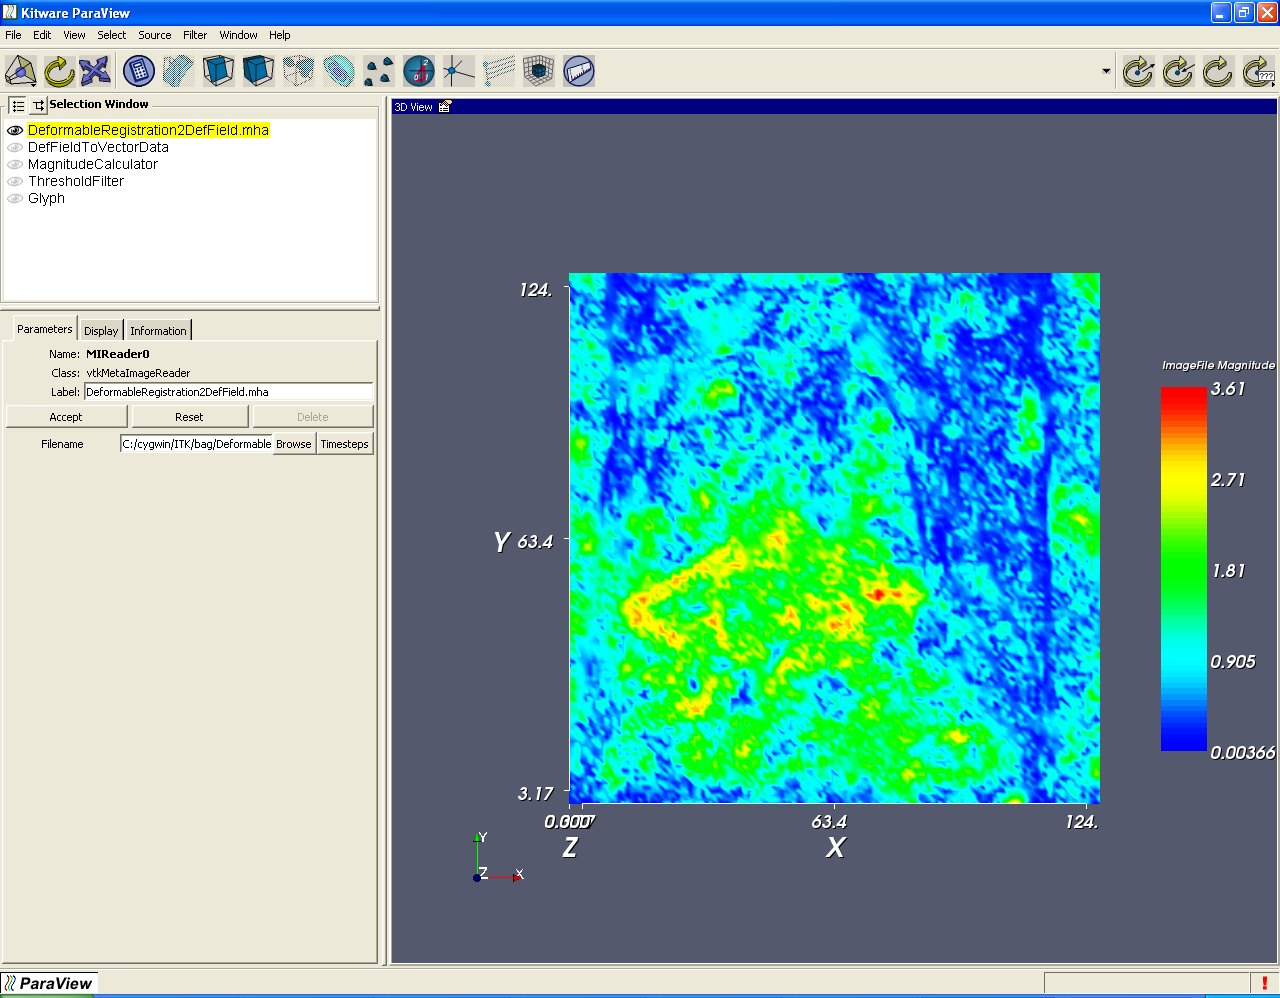
\includegraphics[width=\textwidth]{ParaviewScreenshot1.eps}
\itkcaption[Deformation field magnitudes]{Deformation field magnitudes displayed using Paraview}
\label{fig:ParaviewScreenshot1}
\end{figure}

\begin{figure}
\center
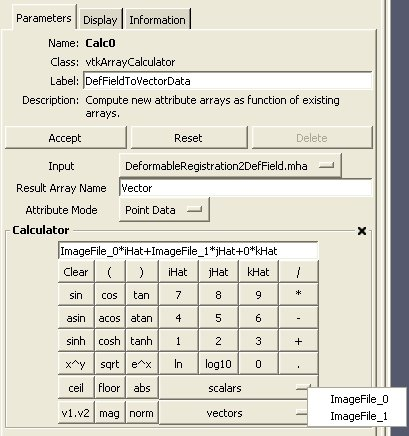
\includegraphics[width=0.3\textwidth]{ParaviewScreenshot2.eps}
\itkcaption[Calculator]{Calculators and filters may be used to compute the vector magnitude, compose vectors etc.}
\label{fig:ParaviewScreenshot2}
\end{figure}

\begin{figure}
\center
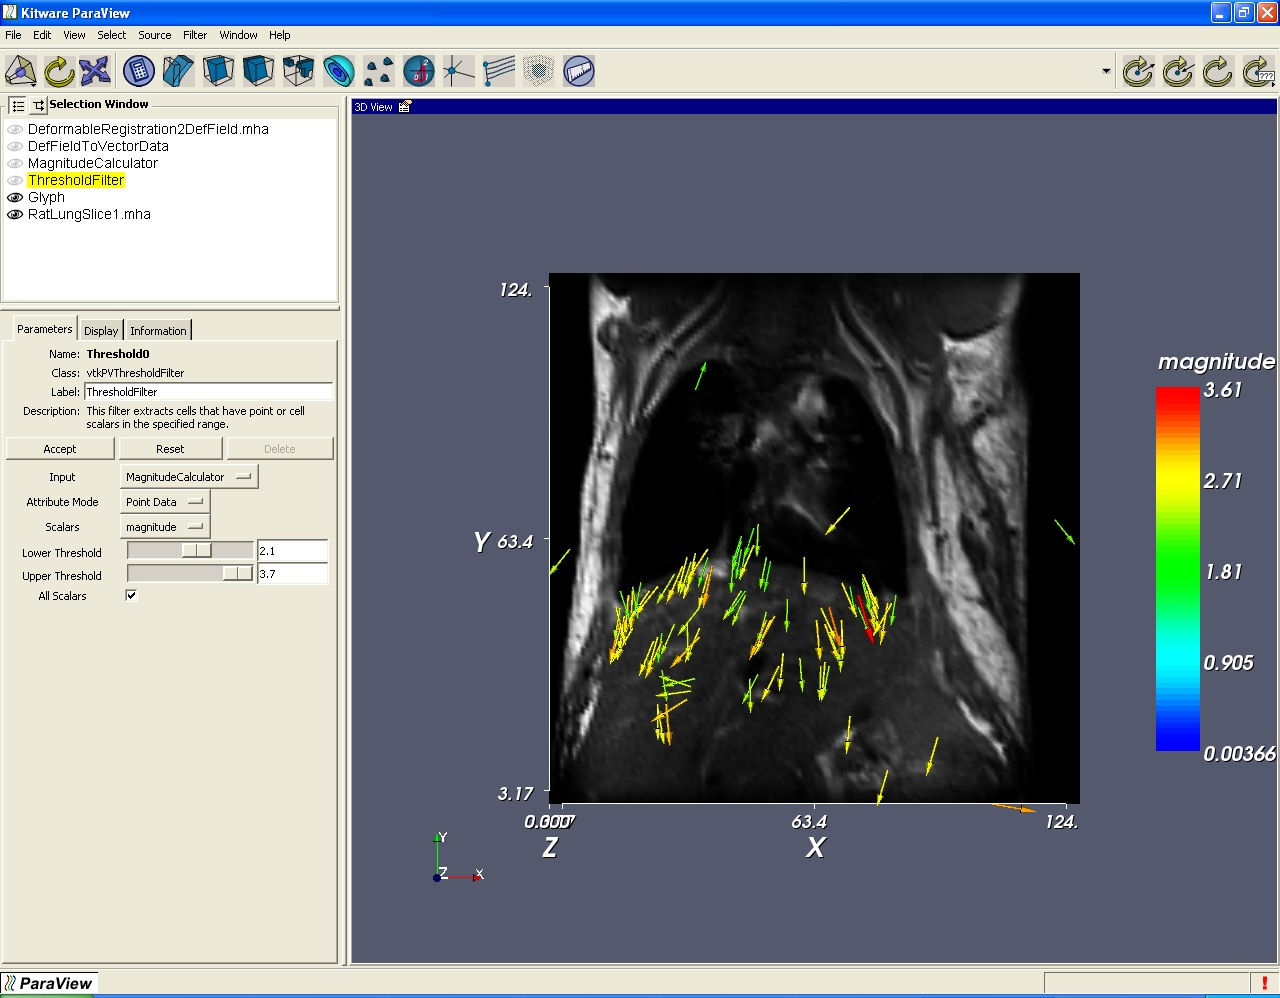
\includegraphics[width=\textwidth]{ParaviewScreenshot3.eps}
\itkcaption[Visualized Def field]{Deformation field visualized using Paraview after thresholding and subsampling.}
\label{fig:ParaviewScreenshot3}
\end{figure}



\subsection{Visualizing 3D deformation fields}
Let us create a 3D deformation field. We will use Thin Plate Splines to warp a 3D dataset and create a deformation field. We will pick a set of point landmarks and translate them to provide a specification of correspondences at point landmarks. Note that the landmarks have been picked randomly for purposes of illustration and are not intended to portray a true deformation. The landmarks may be used to produce a deformation field in several ways. Most techniques minimize some regularizing functional representing the irregularity of the deformation field, which is usually some function of the spatial derivatives of the field. Here will we use {\it thin plate splines}. Thin plate splines minimize the regularizing functional 

\begin{equation}
I[f(x,y)] = \iint (f^2_{xx} + 2 f^2_{xy} + f^2_{yy}) dx dy
\end{equation}
where the subscripts denote partial derivatives of f.

The code for this section can be found in Insight/Examples/Registration/ThinPlateSplineWarp.cxx

We may now proceed as before to visualize the deformation field using Paraview as shown in Figure \ref{fig:ParaviewScreenshot4}.

\begin{figure}
\center
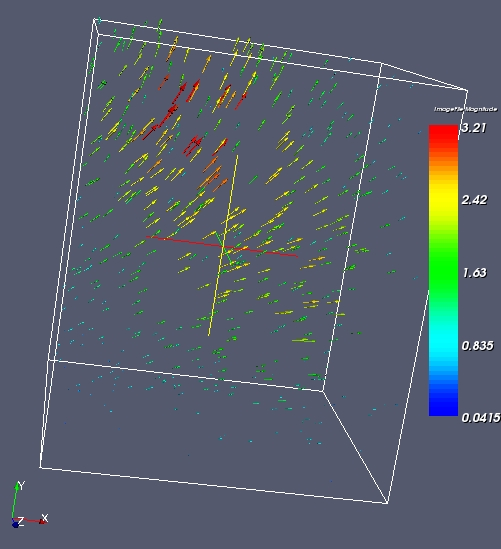
\includegraphics[width=0.7\textwidth]{ParaviewScreenshot4.eps}
\itkcaption[Visualized Def field4]{3D Deformation field visualized using Paraview.}
\label{fig:ParaviewScreenshot4}
\end{figure}




\fi

\ifitkFullVersion
%%%%%%%%%%%%%%%%%%%%%%%%%%%%%%%%%%%%%%%%%%%%%%%%%%%%%%%%%%%%%%%
%
%
%   This file is included in DeformableRegistration.tex
%
%   Labels and section entries are defined in that file.
%
%
%
%%%%%%%%%%%%%%%%%%%%%%%%%%%%%%%%%%%%%%%%%%%%%%%%%%%%%%%%%%%%%%
Let us register the deformed volumes generated by Thin plate warping in the
previous example using DeformableRegistration4.cxx. Since ITK is in general
N-dimensional, the only change in the example is to replace the
\code{ImageDimension} by 3.

The registration method uses B-splines and an LBFGS optimizer. The trace in
Table. \ref{tab:LBFGStrace} prints the trace of the optimizer through the
search space.

\begin{table}
\begin{center}
\begin{tabular}{\tableconfiguration}
\hline
\textbf{Iteration} &
\textbf{Function value} &
\textbf{$\|G\|$} &
\textbf{Step length} \\
\hline\hline
   1    &        156.981  &    14.911  & 0.202 \\
   2    &        68.956    &    11.774    &    1.500 \\
   3    &        38.146    &    4.802     &   1.500 \\
   4    &        26.690    &    2.515     &   1.500 \\
   5    &        23.295    &    1.106     &   1.500\\
   6    &        21.454    &    1.032     &   1.500\\
   7    &        20.322    &    1.557     &   1.500\\
   8    &        19.751    &    0.594     &   1.500\\
\hline
\end{tabular}
\end{center}
\itkcaption[LBFGS Optimizer trace]{LBFGS Optimizer trace.
\label{tab:LBFGStrace}}
\end{table}

Here $\|G\|$ is the norm of the gradient at the current estimate of the
minimum, $x$. ``Function Value" is the current value of the function, f(x).

The resulting deformation field that maps the moving to the fixed image is
shown in \ref{fig:DeformationFieldOutput}. A difference image of two slices
before and after registration is shown in
\ref{fig:DefRegistrationDiffScreenshot}. As can be seen from the figures, the
deformation field is in close agreement to the one generated from the Thin
plate spline warping.

\begin{figure}
\center
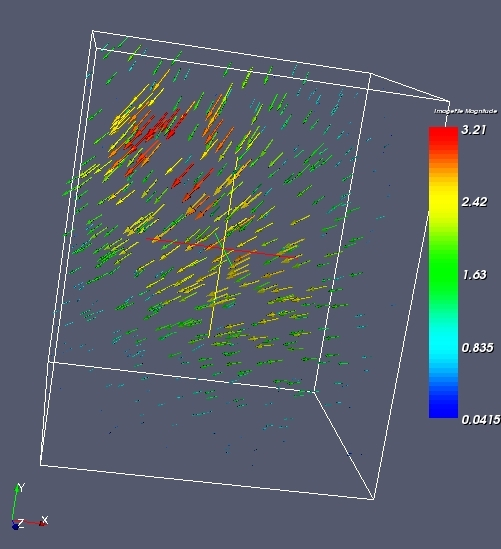
\includegraphics[width=0.6\textwidth]{ParaviewScreenshot5.eps}
\itkcaption[Deformation field output]{Resulting deformation field that maps the moving image to the fixed image.}
\label{fig:DeformationFieldOutput}
\end{figure}

\begin{figure}
\center

\includegraphics[width=0.44\textwidth]{DeformableRegistration4DiffBefore.eps}
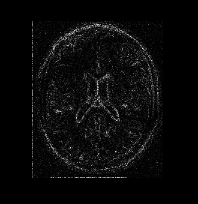
\includegraphics[width=0.44\textwidth]{DeformableRegistration4DiffAfter.eps}
\itkcaption[Difference image]{Difference image from a slice before and after registration.}
\label{fig:DefRegistrationDiffScreenshot}
\end{figure}



\fi


% the clearpage command helps to avoid orphans in the title of the next
% section.
\clearpage

\section{Model Based Registration}
\label{sec:ModelBasedRegistration}
\ifitkFullVersion
%%%%%%%%%%%%%%%%%%%%%%%%%%%%%%%%%%%%%%%%%%%%%%%%%%%%%%%%%%%%%%%
%
%
%   This file is included in Registration.tex
%
%   Lablels and section entries are defined in that file.
%
%
%
%%%%%%%%%%%%%%%%%%%%%%%%%%%%%%%%%%%%%%%%%%%%%%%%%%%%%%%%%%%%%%%

\itkpiccaption[Model to Image Registration Framework Components]{The basic components of model based registration are an image, a spatial object, a transform, a metric, an interpolator and an optimizer.\label{fig:ModelToImageRegistrationComponentsDiagram}}
\parpic(8cm,6cm)[r]{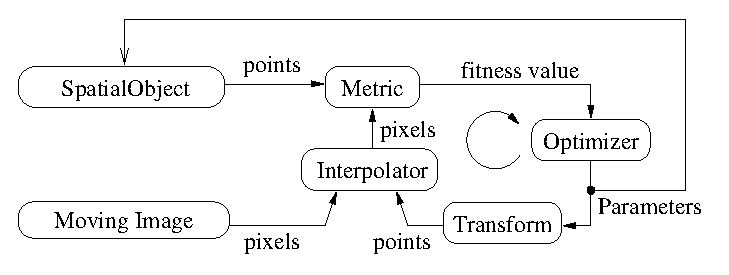
\includegraphics[width=7.5cm]{ModelToImageRegistrationComponentsDiagram.eps}}

This section introduces the concept of registering a geometrical model with an
image. We refer to this concept as \emph{Model Based Registration} but this may
not be the most widespread terminology. In this approach for registration, a
geometrical model is build first and a number of parameters are identified in
the model. Variations of these parameters make possible to adapt the model to
the particular morphology of a specific patient. The task of registration is
then to find the optimal combinations of the model parameters that will make
this model fit as a good representation of the anatomical structure contained
in an image. 


\begin{figure}
\center
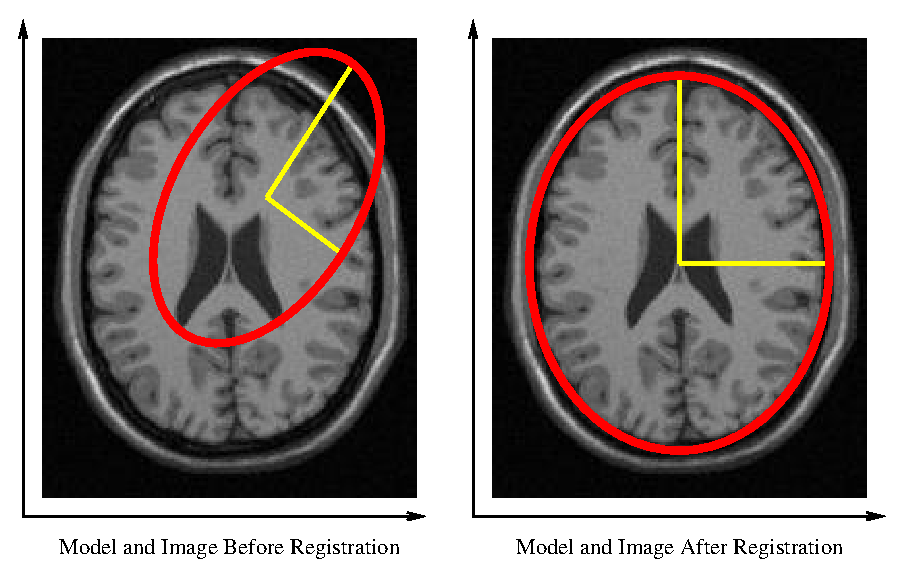
\includegraphics[width=\textwidth]{ModelToImageRegistrationConcept.eps}
\itkcaption[Model to Image Registration Framework Concept]{Basic concept of
  Model-to-Image registration.  A simplified geometrical model (ellipse) is
    registered against an anatomical structure (skull)  by applying a spatial
    transform and modifying the model internal parameters. This image is not
    the result of an actual registration, it is shown here only with the
    purpose of illustrating the concept of model to image registration.}
\label{fig:ModelToImageRegistrationConcept}
\end{figure}


For example, let's say that in the axial view of a brain image we can roughly
approximate the skull with an ellipse. The ellipse becomes our simplified
geometrical model, and registration is the task of finding the best center for
the ellipse, the measures of its axis lengths and its orientation on the plane.
This is illustrated in Figure~\ref{fig:ModelToImageRegistrationConcept}.  If we
compare this aproach with the Image-to-Image registration problem, we can see
that the main difference here is that in addition to mapping the spatial
position of the model, we can also customize internal parameters that change
its shape.

Figure~\ref{fig:ModelToImageRegistrationComponentsDiagram} illustrates the
major components of the registration framework in ITK when a model base
registration problem is configured. The basic input data for the registration
is provided by pixel data in an \doxygen{Image} and by geometrical data stored
in a \doxygen{SpatialObject}. A Metric has to be defined in order to evaluate
the fitness between the model and the image. This fitness value can be improved
by introducing variations in the spatial positioning of the
\doxygen{SpatialObject} and/or by changing its internal parameters. The search
space for the optimizer is now the composition of the transform parameter and
the shape internal parameters.

This same approach can be considered a segmentation technique, since once the
model has been optimally superimposed to the image we could label pixels
according to their associations with specific parts of the model. The
perpectives of model to image registration/segmentation are endless.  Probably
the main advantage of this approach is that, as opposed to image-to-image
registration, it actually provides \emph{Insight} into the anatomical structure
contained in the image. The adapted model becomes a condensed representation of
the essential elements of the anatomical structure.

ITK provides a hierarchy of classes intended to support the construction of
shape models. This hierarchy has the \doxygen{SpatialObject} as its base class.
A number of basic functionalities are defined at this level. For example, the
capacity to evaluate is a given point is \emph{inside} or \emph{outside} of the
model, the capability to form complex shapes by creating hierarchical
conglomerates of basic shapes and the support for basic spatial
parameterizations like scale, orientation and position.

The following sections present examples of the typical uses of these powerful
elements of the toolkit.

%\ifitkFullVersion
\input{ModelToImageRegistration1.tex} 
%\fi





\fi


\section{Point Set Registration}
\label{sec:PointSetRegistration}

The classical algorithm for performing PointSet to PointSet registration is the
Iterative Closest Point (ICP) algorithm.  The following examples illustrate how
this can be used in ITK.

\ifitkFullVersion
\input{IterativeClosestPoint1.tex}
\fi

\ifitkFullVersion
\input{IterativeClosestPoint2.tex}
\fi

\ifitkFullVersion
\input{IterativeClosestPoint3.tex}
\fi



\fi

\ifitkFullVersion

\chapter{Segmentation}

Segmentation of medical images is a challenging task. Myriads of different
methods have been proposed and implemented in recent years. In spite of the
huge effort invested on this problem, there is no a single approach that could
solve in general the problem of segmentation for the large variety of image
modalities existing today.

The most effective segmentation algorithms are obtained by carefully
customizing combination of components. The parameters of these components are
tunned for the characteristics of the image modality used as input and the
features of the anatomical structure to be segmented. 

The Insight toolkit provides a basic set of algorithms that can be used to
develop and customize a full segmentation application. Some of the most
commonly used segmentation components are described in the following sections.


\section{Region Growing}

Region growing algorithms have proved to be a very effective approach for image
segmentation. The basic concept of a region growing algorithm is to start from
a seed region that is considered to belong to the object to be segmented. The
neighbor pixels to this initial region are evaluated to determine if they could
also be considered part of the object, in which case, they are added to the
region. When some of the neighbor pixels are included in the region, other
pixels become new neighbors and hence become candidates to be evaluated and
eventually included in the region. Region growing algorithms vary depending on
the criteria used to decide whether a pixel should be included in the region
or not, the type of neighbor connectivity used on the image grid and the
strategy used for visiting the neighbor pixels.

Several implementations of region growing are available in the
Insight toolkit. This section describes some of the most commonly used.

\subsection{Confidence Connected}
\label{sec:ConfidenceConnected}
\input{ConfidenceConnected.tex}

\subsection{Threshold Connected}

\section{Segmentation Based on Watersheds}
\label{sec:WatershedSegmentation}
\input WatershedSegmentation.tex


%% \section{Level Sets Segmentation}
%% \label{sec:LevelSetsSegmentation}

%% \subsection{Threshold Level Set Segmentation}
%% \subsection{Fast Marching Segmentation}
%% \subsection{Shape Detection Segmentation}
%% \subsection{Geodesic Contours Segmentation}


\section{Hybrid Methods} 
\label{sec:HybridSegmentationMethods}

It is sometimes convenient to combine several segmentation strategies with the
aim of taking advantage of their qualities an compensate their vulnerabilities.
The synergy between fundamentally different methodologies tends to result in
robustness and higher segmentation quality.  This section illustrates an hybrid
approach for segmentation in which two different strategies are configured to
work together. In this case, an input image is first processed by a filter
based on the concept of region growing. The criterion of acceptance in the
region is defined by a similarity measure that evaluates how homogeneous is the
path between to pixels. The output of this filter is used as a prior for
another filter that performs a full partition of the image space and then work
joining and splitting regions in order to optimize an homogeneity measure.
Details on the concepts behind those methods have been discussed in the
litterature
\cite{Angelini2002,Udupa2002,Jin2002,Imielinska2001,Imielinska2000a,Imielinska2000b}

\input{HybridSegmentationFuzzyVoronoi.tex}




\fi

\ifitkFullVersion
\chapter{Statistics}
\label{sec:StaisticsFramework}

This chapter introduces the statistics functionalities in Insight. The
statistics subsystem's primary purpose is to provide general capabilities
for statistical pattern classification. However, its use is not limited
for classification. Users might want to use data containers and
algorithms in the statistics subsystem to perform other statistical
analysis or to preprocessor image data for other tasks.

The statistics subsystem mainly consists of three parts: data container
classes, statistical algorithms, and the classification framework. In this
chapter, we will discuss each major part in that order.

\section{Data Containers}
\label{sec:StatisticsDataContainer}

An \subdoxygen{Statistics}{Sample} object is a data container of elements
that we call \emph{measurement vectors}. A measurement vector is an array of
values (of the same type) measured on an object (In images, it can be a
vector of the gray intensity value and/or the gradient value of a
pixel). Strictly speaking from the design of the Sample class, a measurement
vector can be any class derived from \doxygen{FixedArray}, including
FixedArray itself.

\begin{figure}
  \centering
  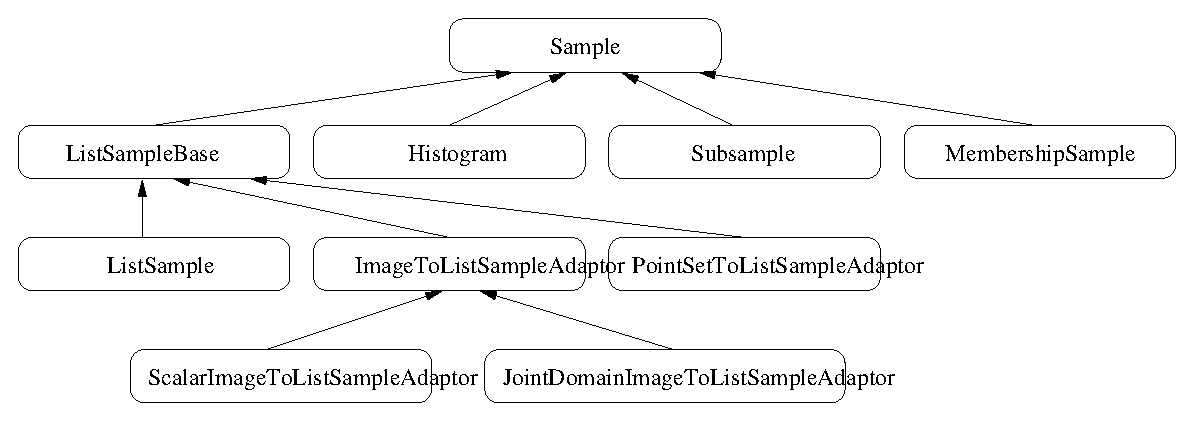
\includegraphics[width=0.9\textwidth]{SampleInheritanceTree.eps}
  \itkcaption[Sample class inheritance tree]{Sample class inheritance diagram.}
  \protect\label{fig:SampleInheritanceTree}
\end{figure}

\subsection{Sample Interface}
\label{sec:SampleInterface}

\ifitkFullVersion 
\input{ListSample.tex}
\fi

\subsection{Sample Adaptors}
\label{sec:SampleAdaptors}

There are two adaptor classes that provide the common
\subdoxygen{Statistics}{Sample} interfaces for \doxygen{Image} and
\doxygen{PointSet}, two fundamental data container classes found in ITK. The
adaptor classes do not store any real data elements themselves. These data
comes from the source data container plugged into them. First, we will
describe how to create an
\subdoxygen{Statistics}{ImageToListAdaptor} and then an
\subdoxygen{statistics}{PointSetToListAdaptor} object.

\subsubsection{ImageToListAdaptor}
\label{sec:ImageToListAdaptor}

\ifitkFullVersion 
\input{ImageToListAdaptor.tex}
\fi

\subsubsection{PointSetToListAdaptor}
\label{sec:PointSetToListAdaptor}

\ifitkFullVersion 
\input{PointSetToListAdaptor.tex}
\fi

\ifitkFullVersion 
\input{PointSetToAdaptor.tex}
\fi


\subsection{Histogram}
\label{sec:Histogram}

\ifitkFullVersion 
\input{Histogram.tex}
\fi

\subsection{Subsample}
\label{sec:Subsample}

\ifitkFullVersion 
\input{Subsample.tex}
\fi

\subsection{MembershipSample}
\label{sec:MembershipSample}

\ifitkFullVersion 
\input{MembershipSample.tex}
\fi

\subsection{MembershipSampleGenerator}
\label{sec:MembershipSampleGenerator}

\ifitkFullVersion 
\input{MembershipSampleGenerator.tex}
\fi


\subsection{K-d Tree}
\label{sec:KdTree}

\ifitkFullVersion 
\input{KdTree.tex}
\fi

\section{Algorithms and Functions}
\label{sec:StatisticsAlgorithmsFunctions}

In the previous section, we described the data containers in the ITK
statistics subsystem. We also need data processing algorithms and statistical
functions to conduct statistical analysis or statistical classification using
these containers. Here we define an algorithm to be an operation over a set
of measurement vectors in a sample. A function is an operation over
individual measurement vectors. For example, if we implement a class
(\subdoxygen{Statistics}{EuclideanDistance}) to calculate the Euclidean
distance between two measurement vectors, we call it a function, while if we
implemented a class (\subdoxygen{Statistics}{MeanCalculator}) to calculate
the mean of a sample, we call it an algorithm.

\subsection{Sample Statistics}
\label{sec:SampleStatistics}

We will show how to get sample statistics such as means and covariance from
the (\subdoxygen{Statistics}{Sample}) classes. Statistics can tells us
characteristics of a sample. Such sample statistics are very important for
statistical classification. When we know the form of the sample distributions
and their parameters (statistics), we can conduct Bayesian classification. In
ITK, sample mean and covariance calculation algorithms are implemented. Each
algorithm also has its weighted version (see Section
\ref{sec:WeightedMeanCovariance}). The weighted versions are used in the
expectation-maximization parameter estimation process.

\subsubsection{Mean and Covariance}
\label{sec:MeanCovariance}

\ifitkFullVersion 
\input{SampleStatistics.tex}
\fi

\subsubsection{Weighted Mean and Covariance}
\label{sec:WeightedMeanCovariance}

\ifitkFullVersion 
\input{WeightedSampleStatistics.tex}
\fi

\subsection{Sample Generation}
\label{sec:SampleGeneration}

\subsubsection{ListSampleToHistogramFilter}
\label{sec:ListSampleToHistogramFilter}

\ifitkFullVersion 
\input{ListSampleToHistogramFilter.tex}
\fi

\subsubsection{ListSampleToHistogramGenerator}
\label{sec:ListSampleToHistogramGenerator}

\ifitkFullVersion 
\input{ListSampleToHistogramGenerator.tex}
\fi

\subsubsection{NeighborhoodSampler}
\label{sec:NeighborhoodSampler}

\ifitkFullVersion 
\input{NeighborhoodSampler.tex}
\fi

\subsubsection{SampleToHistogramProjectionFilter}
\label{sec:SampleToHistogramProjectionFilter}

\ifitkFullVersion 
\input{SampleToHistogramProjectionFilter.tex}
\fi




\subsection{Sample Sorting}
\label{sec:SampleSorting}

\ifitkFullVersion 
\input{SampleSorting.tex}
\fi

\subsection{Probability Density Functions}
\label{sec:ProbabilityDensityFunctions}

The probability density function (PDF) for a specific distribution returns
the probability density for a measurement vector. To get the probability
density from a PDF, we use the \code{Evaluate(input)} method. PDFs for
different distributions require different sets of distribution
parameters. Before calling the \code{Evaluate()} method, make sure to set the
proper values for the distribution parameters.

\subsubsection{Gaussian Distribution}
\label{sec:GaussianDensityFunction}

\ifitkFullVersion 
\input{GaussianDensityFunction.tex}
\fi

\subsection{Distance Metric}
\label{sec:DistanceMetric}

\subsubsection{Euclidean Distance}
\label{sec:EuclideanDistance}

\ifitkFullVersion 
\input{EuclideanDistance.tex}
\fi

\subsection{Decision Rules}
\label{sec:DecisionRules}

A decision rule is a function that returns the index of one data element in a
vector of data elements. The index returned depends on the internal logic of
each decision rule. The decision rule is an essential part of the ITK
statistical classification framework. The scores from a set of membership
functions (e.g. probability density functions, distance metrics) are compared
by a decision rule and a class label is assigned based on the output of the
decision rule. The common interface is very simple. Any decision rule class
must implement the \code{Evaluate()} method. In addition to this method,
certain decision rule class can have additional method that accepts prior
knowledge about the decision task. The
\doxygen{MaximumRatioDecisionRule} is an example of such a class.

The argument type for the \code{Evaluate()} method is
\code{std::vector< double >}. The decision rule classes are part of the
\code{itk} namespace instead of \code{itk::Statistics} namespace.

For a project that uses a decision rule, it must link the \code{itkCommon}
library. Decision rules are not templated classes.

\subsubsection{Maximum Decision Rule}
\label{sec:MaximumDecisionRule}

\ifitkFullVersion 
\input{MaximumDecisionRule.tex}
\fi

\subsubsection{Minimum Decision Rule}
\label{sec:MinimumDecisionRule}

\ifitkFullVersion 
\input{MinimumDecisionRule.tex}
\fi

\subsubsection{Maximum Ratio Decision Rule}
\label{sec:MaximumRatioDecisionRule}

\input{MaximumRatioDecisionRule.tex}

\subsection{Random Variable Generation}
\label{sec:RandomVariableGeneration}

A random variable generation class returns a variate when the
\code{GetVariate()} method is called. When we repeatedly call the method
for ``enough'' times, the set of variates we will get follows
the distribution form of the random variable generation class.
 
\subsubsection{Normal (Gaussian) Distribution}
\label{sec:NormalVariateGeneration}

\ifitkFullVersion 
\input{NormalVariateGenerator.tex}
\fi


\section{Statistics applied to Images}
\label{sec:StatisticsAppliedToImages}

\subsection{Image Histograms}
\label{sec:ImageHistogram}


\subsubsection{Scalar Image Histogram with Adaptor}
\label{sec:ScalarImageHistogramAdaptor}
\ifitkFullVersion 
\input{ImageHistogram1.tex}
\fi


\subsubsection{Scalar Image Histogram with Generator}
\label{sec:ScalarImageHistogramGenerator}
\ifitkFullVersion 
\input{ImageHistogram2.tex}
\fi


\subsubsection{Color Image Histogram with Generator}
\label{sec:ColorImageHistogramGenerator}
\ifitkFullVersion 
\input{ImageHistogram3.tex}
\fi


\subsubsection{Color Image Histogram Writing}
\label{sec:ColorImageHistogramGeneratorWriting}
\ifitkFullVersion 
\input{ImageHistogram4.tex}
\fi


\subsection{Image Information Theory}
\label{sec:ComputingImageEntropy}

Many concepts from Information Theory have been used successfully in the domain
of image processing. This section introduces some of such concepts and
illustrates how the statistical framework in ITK can be used for computing
measures that have some relevance in terms of Information Theory
\cite{Shannon1948,Shannon1949,Kullback1997}.


\subsubsection{Computing Image Entropy}
\label{sec:ComputingImageEntropy}

\index{Entropy!What's wrong in images}

The concept of Entropy has been introduced into image processing as a crude
mapping from its application in Communications. The notions of Information
Theory can be decepting and misleading when applied to images because their
language from Communication Theory does not necessarily maps to what people in
the Imaging Community use.

For example, it is commonly said that

\emph{``The Entropy of an image is a measure of the amount of information
contained in an image''}. 

This statement is fundamentally \textbf{incorrect}. 

The way the notion of Entropy is commonly measured in images is by first
assuming that the spatial location of a pixel in an image is irrelevant!  That
is, we simply take the statistical distribution of the pixel values as it can
be evaluated in a histogram and from that histogram we estimate the frequency
of the value associated to each bin. In other words, we simply assume that the
image is a set of pixels that are passing through a channel, just as things are
commonly considered for communication purposes.

Once the frequency of every pixel value has been estimated, Information Theory
defines that the amount of uncertainty that an observer will lose by taking one
pixel and finding its real value to be the one associated with the i-th bin of the
histogram, is given by $-\log_2{(p_i)}$, where $p_i$ is the frequency in that
histogram bin. Since a reduction in uncertainty is equivalent to an increase in
the amount of information in the observer, we conclude that measuring one pixel
and finding its level to be in the i-th bin results in an acquisition of
$-\log_2{(p_i)}$ bits of information\footnote{Note that \textbf{bit} is the unit of
amount of information. Our modern culture has vulgarized the bit and its
multiples, the Byte, KiloByte, MegaByte, GigaByte and so on as simple measures
of the amount of RAM memory and capacity of a hard drive in a computer. In that
sense, a confusion is created between the encoding of a piece of data and its
actual amount of information. For example a file composed of one million
letters will take one million bytes in a hard disk, but it does not necessariy
has one million bytes of information, since in many cases parts of the file can
be predicted from others. This is the reason why data compression can manage to
compact files.}.

Since we could have picked any pixel at random, our chances or picking the ones
that are associated to the i-th histogram bin are given by $p_i$. Therefore,
the expected reduction in uncertainty that we can get from measuring the value
of one pixel is given by

\begin{equation}
H = - \sum_i{ p_i  \cdot \log_2{(p_i)} }
\end{equation}

This quantity $H$ is what is usually defined as the \emph{Entropy of the
Image}. It would be more accurate to call it the Entropy of the random variable
associated to the intensity value of \emph{one} pixel. The fact that $H$ is
unrelated to the spatial arrangement of the pixels in an image shows how little
of the real \emph{Image Information} is $H$ actually representing. The Entropy
of an image, as mesure above, is only a crude indication of how the intensity
values are spread in the dynamic range of intensites. For example, an image
with maximum entropy will be the one that has a large dynamic range and every
value in that range is equally probable. 

The common acceptation of $H$ as a representation of image information has
terribly undermined the enormous potential on the application of Information
Theory to image processing and analysis.

The real concepts of Information Theory would require that we define the amount
of information in an image based on our expectations and prior knowledge from
that image. In particular, the \emph{Amount of Information} provided by an
image should measure the number of features that we are not able to predict
based on our prior knowledge about that image. For example, if we know that we
are going to analyze a CT scan of the abdomen of an adult human male in the age
range of 40 to 45, there is already a good deal that we could predict about the
content of that image.  The real amount of information in the image is the
representation of the features in the image that we could not predict from
knowing that it is a CT scan from a human adult male.

The application of Information Theory to image analysis is still in its early
infancy and it is an exciting an promising field to be explored further. All
that being said, let's now look closer at how the concept of Entropy (which is
not the amount of information in an image) can be measured with the ITK
statistics framework.

\ifitkFullVersion 
\input{ImageEntropy1.tex}
\fi

\subsubsection{Computing Images Mutual Information}
\label{sec:ComputingImagesMutualInformation}

\ifitkFullVersion 
\input{ImageMutualInformation1.tex}
\fi



\section{Classification}
\label{sec:Classification}

In statistical classification, each object is represented by $d$ features (a
measurement vector), and the goal of classification becomes finding compact and
disjoint regions (decision regions\cite{Duda2000}) for classes in a
$d$-dimensional feature space. Such decision regions are defined by decision
rules that are known or can be trained.  The simplest configuration of a
classification consists of a decision rule and multiple membership functions;
each membership function represents a class. Figure~\ref{fig:simple}
illustrates this general framework.

\begin{figure}[h]
  \centering
  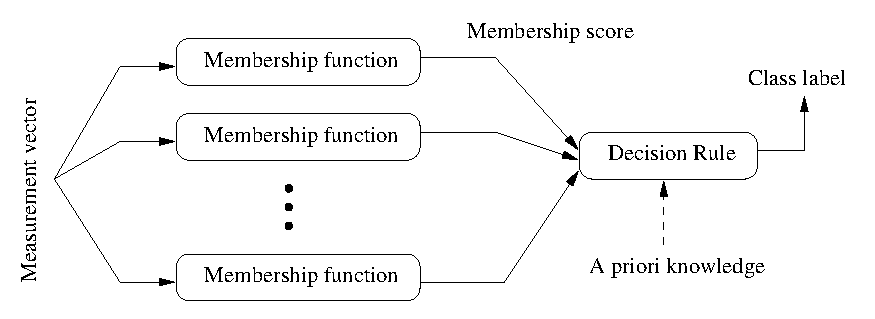
\includegraphics[width=0.7\textwidth]{DudaClassifier.eps}
  \itkcaption[Simple conceptual classifier]{Simple conceptual classifier.}
  \label{fig:simple}
\end{figure}

This framework closely follows that of Duda and
Hart\cite{Duda2000}. The classification process can be described
as follows:

\begin{enumerate}
\item{A measurement vector is input to each membership function.}
\item{Membership functions feed the membership scores to the
    decision rule.}
\item{A decision rule compares the membership scores and returns a
    class label.}
\end{enumerate}

\begin{figure}
  \centering
  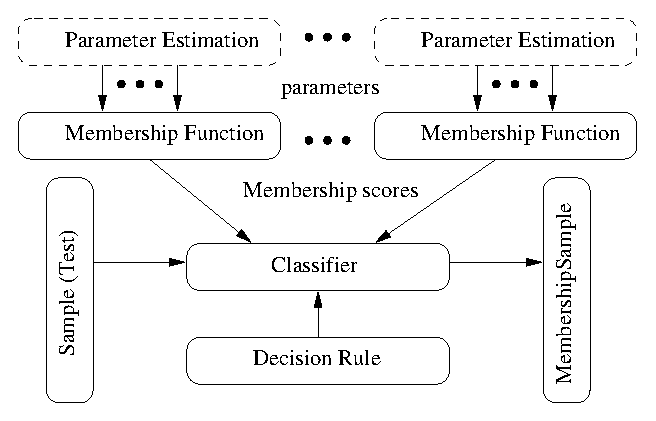
\includegraphics[width=0.7\textwidth]{StatisticalClassificationFramework.eps}
  \itkcaption[Statistical classification framework]{Statistical classification
framework.}
  \protect\label{fig:StatisticalClassificationFramework}
\end{figure}

This simple configuration can be used to formulated various classification
tasks by using different membership functions and incorporating task specific
requirements and prior knowledge into the decision rule. For example, instead
of using probability density functions as membership functions, through
distance functions and a minimum value decision rule (which assigns a class
from the distance function that returns the smallest value) users can achieve a
least squared error classifier. As another example, users can add a rejection
scheme to the decision rule so that even in a situation where the membership
scores suggest a ``winner'', a measurement vector can be flagged as ill
defined. Such a rejection scheme can avoid risks of assigning a class label
without a proper win margin.

\subsection{k-d Tree Based k-Means Clustering}
\label{sec:KdTreeBasedKMeansClustering}
\ifitkFullVersion
\input{KdTreeBasedKMeansClustering.tex}
\fi

\subsection{K-Means Classification}
\label{sec:KMeansClassifier}
\ifitkFullVersion
\input{ScalarImageKmeansClassifier.tex}
\fi

\subsection{Bayesian Plug-In Classifier}
\label{sec:BayesianPluginClassifier}

\ifitkFullVersion 
\input{BayesianPluginClassifier.tex}
\fi


\subsection{Expectation Maximization Mixture Model Estimation}
\label{sec:ExpectationMaximizationMixtureModelEstimation}

\ifitkFullVersion 
\input{ExpectationMaximizationMixtureModelEstimator.tex}
\fi

\subsection{Classification using Markov Random Field}
\label{sec:MarkovRandomField}

Markov Random Fields are probabilistic models that use the correlation between
pixels in a neighborhood to decide the object region. The
\subdoxygen{Statistics}{MRFImageFilter} uses the maximum a posteriori (MAP)
estimates for modeling the MRF. The object traverses the data set and uses the
model generated by the Mahalanobis distance classifier to gets the the distance
between each pixel in the data set to a set of known classes, updates the
distances by evaluating the influence of its neighboring pixels (based on a MRF
model) and finally, classifies each pixel to the class which has the minimum
distance to that pixel (taking the neighborhood influence under consideration).
The energy function minimization is done using the iterated coditional modes
(ICM) algorithm \cite{Besag1986}.

\ifitkFullVersion
\input{ScalarImageMarkovRandomField1.tex}
\fi 




\fi

%%% \chapter{Application}

Pointers and a brief description of the available ITK applications.




\ifitkFullVersion
\part{Developer's Guide}

%%% \chapter{Infrastructure.tex}

Smart pointers, exceptions, events, object factories

\chapter{Iterators}

Using iterators in algorithms: image and mesh

\chapter{How To Write A Filter}
\label{chapter:WriteAFilter}

This purpose of this chapter is help developers create their own
filter (process object).  This chapter is divided into four major
parts. An initial definition of terms is followed by an overview of
the filter creation process. Next, data streaming is discussed. The
way data is streamed in ITK must be understood in order to write
correct filters. Finally, a section on multithreading describes what
you must do in order to take advantage of shared memory parallel
processing.

\section{Terminology}
\label{sec:Terminology}

The following is some basic terminology for the discussion that follows.
Chapter \ref{chapter:SystemOverview} provides additional background
information.

\begin{itemize}
        \item The \textbf{data processing pipeline} is a directed graph of
        \textbf{process} and \textbf{data objects}. The pipeline inputs,
        operators on, and outputs data.
        \index{data processing pipeline}
        \index{process object}
        \index{data object}

        \item A \textbf{filter}, or \textbf{process object}, has one or more
        inputs, and one or more outputs.
        \index{filter}

        \item A \textbf{source}, or source process object, initiates the data
        processing pipeline, and has one or more outputs.
        \index{source}

        \item A \textbf{mapper}, or mapper process object, terminates the
        data processing pipeline. The mapper has one or more outputs, and may
        write data to disk, interface with a display system, or interface to
        any other system.
        \index{mapper}

        \item A \textbf{data object} represents and provides access to
        data. In ITK, the data object (ITK class \doxygen{DataObject}) is 
        typically of type \doxygen{Image} or \doxygen{Mesh}.
        \index{data object}

        \item A \textbf{region} (ITK class \doxygen{Region}) represents a 
        piece, or subset of the entire data set.
        \index{region}

        \item An \textbf{image region} (ITK class \doxygen{ImageRegion})
        represents a structured portion of data. ImageRegion is implemented
        using the \doxygen{Index} and \doxygen{Size} classes
        \index{image region}

        \item A \textbf{mesh region} (ITK class \doxygen{MeshRegion}) 
        represents an unstructured portion of data.
        \index{mesh region}

        \item The \textbf{LargestPossibleRegion} is the theoretical single,
        largest piece (region) that could represent the entire dataset. The
        LargestPossibleRegion is used in the system as the measure of the
        largest possible data size.
        \index{LargestPossibleRegion}

        \item The \textbf{BufferedRegion} is a contiguous block of memory
        that is lesss than or equal to in size to the
        LargestPossibleRegion. The buffered region is what has actually been
        allocated by a filter to hold its output.
        \index{BufferedRegion}

        \item The \textbf{RequestedRegion} is the piece of the dataset that a
        filter is required to produce. The RequestedRegion is less than or
        equal in size to the BufferedRegion. The RequestedRegion may differ
        in size from the BufferedRegion due to performance reasons. The
        RequestedRegion may be set by a user, or by an application that needs
        just a portion of the data.
        \index{RequestedRegion}

        \item The \textbf{modified time} (represented by ITK class
        \doxygen{TimeStamp}) is a monotonically increasing integer value that
        characterizes a point in time when an object was last modified.
        \index{modified time}

        \item \textbf{Downstream} is the direction of dataflow, from sources
        to mappers.
        \index{pipeline!downstream}

        \item \textbf{Upstream} is the opposite of downstream, from mappers
        to sources.
        \index{pipeline!upstream}

        \item The \textbf{pipeline modified time} for a particular data
        object is the maximum modified time of all upstream data objects and
        process objects.
        \index{pipeline!modified time}

        \item The term \textbf{information} refers to metadata that
        characterizes data. For example, index and dimensions are information
        characterizing an image region.
        \index{pipeline!information}
\end{itemize}

\section{Overview of Filter Creation}
\label{sec:OverviewFilterCreation}
\index{filter!overview of creation}

\itkpiccaption[Relationship between DataObjects and ProcessObjects]
{Relationship between DataObject and ProcessObject.
\label{fig:DataPipeLineOneConnection}}
\parpic(7cm,2.5cm)[r]{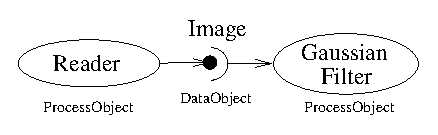
\includegraphics[width=6cm]{DataPipelineOneConnection.eps}}


Filters are defined with respect to the type of data they input (if
any), and the type of data they output (if any). The key to writing a
ITK filter is to identify the number and types of input and
output. Having done so, there are often superclasses that simplify
this task via class derivation. For example, most filters in ITK take
a single image as input, and produce a single image on output. The
superclass \doxygen{ImageToImageFilter} is a convenience class that
provide most of the functionality needed for such a filter.

Once the appropriate superclass is identified, the filter writer
implements the class defining the methods required by most all ITK
objects: \code{New()}, \code{PrintSelf()}, and protected constructor,
copy constructor, delete, and operator=, and so on. Also, don't forget
standard typedefs like \code{Self}, \code{Superclass}, \code{Pointer}, and
\code{ConstPointer}. Then the filter writer can focus on the most important
parts of the implementation: defining the API, data members, and other
implementation details of the algorithm. In particular, the filter writer
will have to implement either a \code{GenerateData()} (non-threaded) or
\code{ThreadedGenerateData()} method. (See Section~\ref{sec:MultiThreading}
for an overview of multi-threading in ITK.)

An important note: the GenerateData() method is required to allocate memory
for the output. The ThreadedGenerateData() method is not. In default
implementation (see \doxygen{ImageSource}, a superclass of
\doxygen{ImageToImageFilter})
\code{GenerateData()} allocates memory and then invokes
\code{ThreadedGenerateData()}.

One of the most important decisions that the developer must make is whether
the filter can stream data; that is, process just a portion of the input to
produce a portion of the output. Often superclass behavior works well: if the
filter processes the input using single pixel access, then the default
behavior is adequate. If not, then the user may have to a) find a more
specialized superclass to derive from, or b) override one or more methods
that control how the filter operates during pipeline execution. The next
section describes these methods.



\section{Streaming Large Data}
\label{sec:StreamingLargeData}
\index{pipeline!streaming large data}

The data associated with multi-dimensional images is large and becoming larger.
This trend is due to advances in scanning resolution, as well as increases in
computing capability. Any practical segmentation and registration software
system must address this fact in order to be useful in application. ITK
addresses this problem via its data streaming facility.

In ITK, streaming is the process of dividing data into pieces, or regions,
and then processing this data through the data pipeline. Recall that the
pipeline consists of process objects that generate data objects, connected
into a pipeline topology. The input to a process object is a data object
(unless the process initiates the pipeline and then it is a source process
object). These data objects in turn are consumed by other process objects,
and so on, until a directed graph of data flow is constructed. Eventually the
pipeline is terminated by one or more mappers, that may write data to
storage, or interface with a graphics or other system. This is illustrated in 
figures \ref{fig:DataPipeLineOneConnection} and \ref{fig:DataPipeLine}.

A significant benefit of this architecture is that the relatively complex
process of managing pipeline execution is designed into the system. This
means that keeping the pipeline up to date, executing only those portions of
the pipeline that have changed, multithreading execution, managing memory
allocation, and streaming is all built into the architecture. However, these
features do introduce complexity into the system, the bulk of which is seen
by class developers. The purpose of this chapter is to describe the pipeline
execution process in detail, with a focus on data streaming.


\subsection{Overview of Pipeline Execution}
\label{sec:OverviewPipelineExecution}
\index{pipeline!overview of execution}

The pipeline execution process performs several important functions.

\begin{figure}
  \par\centering
  \resizebox{5in}{!}{ 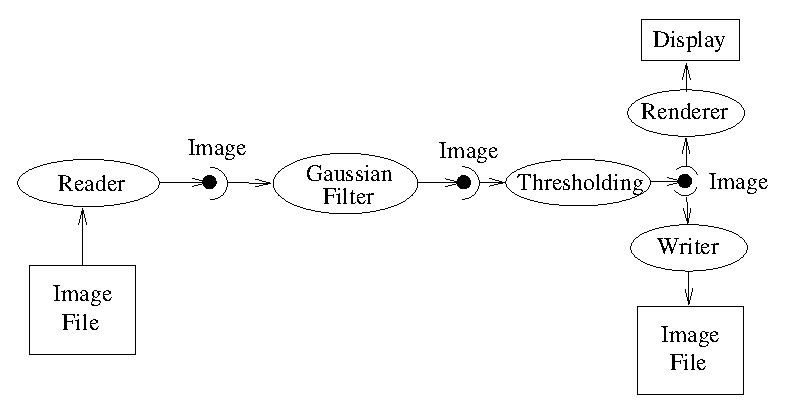
\includegraphics{DataPipeline.eps}} 
  \itkcaption[The Data Pipeline]{The Data Pipeline}
  \label{fig:DataPipeLine}
  \par
\end{figure}

\begin{enumerate}
        \item It determines which filters, in a pipeline of filters, need to
        execute. This prevents redundant execution and minimizes overall
        execution time.

        \item It initializes the (filter's) output data objects, preparing
        them for new data.  In addition, it determines how much memory each
        filter must allocate for its output, and allocates it.

        \item The execution process determines how much data a filter must
        process in order to produce an output of sufficient size for
        downstream filters; it also takes into account any limits on memory
        or special filter requirements. Other factors include the size of
        data processing kernels, that affect how much data input data 
        (extra padding) is required.

        \item It subdivides data into subpieces for multithreading. (Note
        that the division of data into subpieces is exactly same problem as
        dividing data into pieces for streaming; hence multithreading comes
        for free as part of the streaming architecture.)

        \item It may free (or release) output data if filters no longer need
        it to compute, and the user requests that data is to be
        released. (Note: a filter's output data object may be considered a
        ``cache''. If the cache is allowed to remain (\code{ReleaseDataFlagOff()}) 
        between pipeline execution, and the filter, or the input to the 
        filter, never changes, then process objects downstream of the filter 
        just reuse the filter's cache to reexecute.)
\end{enumerate}

To perform these functions, the execution process negotiates with the
filters that define the pipeline. Only each filter can know how much data is
required on input to produce a particular output. For example, a shrink
filter with a shrink factor of two requires an image twice as large (in terms
of its x-y dimensions) on input to produce a particular size output. An
image convolution filter would require extra input (boundary padding)
depending on the size of the convolution kernel. Some filters require the
entire input to produce an output (for example, a histogram), and have the
option of requesting the entire input. (In this case streaming does not work
unless the developer creates a filter that can request multiple pieces,
caching state between each piece to assemble the final output.)


\begin{figure}
  \par\centering
  \resizebox{5in}{!}{ 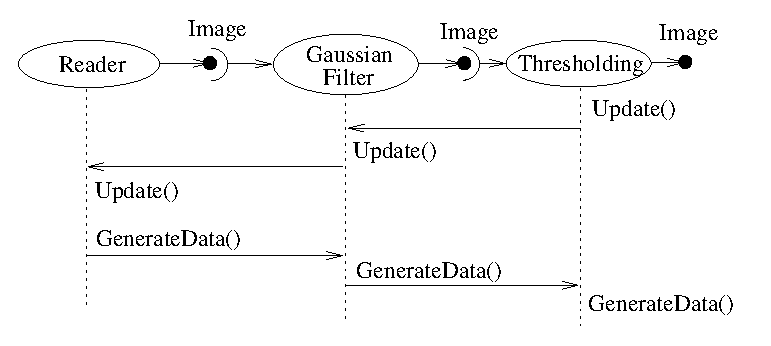
\includegraphics{DataPipelineUpdate.eps}} 
  \itkcaption[Sequence of the Data Pipeline updating mechanism]{Sequence of the
Data Pipeline updating mechanism}
  \label{fig:DataPipeLineUpdate}
  \par
\end{figure}


Ultimately the negotiation process is controlled by the request for data of a
particular size (i.e., region). It may be that the user asks to process a
region of interest within a large image, or that memory limitations result in
processing the data in several pieces. For example, an application may
compute the memory required by a pipeline, and then use
\doxygen{StreamingImageFilter} to break the data processing into several pieces.
The data request is propagated through the pipeline in the upstream
direction, and the negotiation process configures each filter to produce
output data of a particular size.

The secret to creating a streaming filter is to understand how this
negotiation process works, and how to override its default behavior by using
the appropriate virtual functions defined in \doxygen{ProcessObject}. The next
section describes the specifics of these methods, and when to override
them. Examples are provided along the way to illustrate concepts.


\subsection{Details of Pipeline Execution}
\label{sec:DetailsPipelineExecution}
\index{pipeline!execution details}

Typically pipeline execution is initiated when a process object
receives the \code{ProcessObject::Update()} method invocation. This
method is simply delegated to the output of the filter, invoking the
\code{DataObject::Update()} method. Note that this behavior is typical
of the interaction between ProcessObject and DataObject: a method
invoked on one is eventually delegated to the other. In this way the
data request from the pipeline is propagated upstream, initiating data
flow that returns downstream.

The \code{DataObject::Update()} method in turn invokes three other methods:

\begin{itemize}
        \item \code{DataObject::UpdateOutputInformation()}
        \item \code{DataObject::PropagateRequestedRegion()}
        \item \code{DataObject::UpdateOutputData()}
\end{itemize}

\subsubsection{UpdateOutputInformation()}
\label{sec:UpdateOutputInformation}
\index{pipeline!UpdateOutputInformation}

The \code{UpdateOutputInformation()} method determines the pipeline modified
time. It may set the RequestedRegion and the LargestPossibleRegion depending
on how the filters are configured. (The RequestedRegion is set to process all
the data, i.e., the LargestPossibleRegion, if it has not been set.) The
UpdateOutputInformation() propagates upstream through the entire pipeline and
terminates at the sources.

During \code{UpdateOutputInformation()}, filters have a chance to override the
\code{ProcessObject::GenerateOutputInformation()} method
(\code{GenerateOutputInformation()} is invoked by
\code{UpdateOutputInformation()}). The default behavior is for the
\code{GenerateOutputInformation()} to copy the metadata describing the input
to the output (via \code{DataObject::CopyInformation()}). Remember, information
is metadata describing the output, such as the origin, spacing,
and LargestPossibleRegion (i.e., largest possible size) of an image.

A good example of this behavior is \doxygen{ShrinkImageFilter}. This filter
takes an input image and shrinks it by some integral value. The result is that
the spacing and LargestPossibleRegion of the output will be different to that 
of the input. Thus, \code{GenerateOutputInformation()} is overloaded.

\subsubsection{PropagateRequestedRegion()}
\label{sec:PropagateRequestedRegion}
\index{pipeline!PropagateRequestedRegion}

The \code{PropagateRequestedRegion()} call propagates upstream to 
satisfy a data request. In typical application this data request is usually the
LargestPossibleRegion, but if streaming is necessary, or the user is
interested in updating just a portion of the data, the RequestedRegion may be
any valid region within the LargestPossibleRegion.

The function of \code{PropagateRequestedRegion()} is, given a request
for data (the amount is specified by RequestedRegion), propagate
upstream configuring the filter's input and output process object's to
the correct size. Eventually, this means configuring the
BufferedRegion, that is the amount of data actually allocated.

The reason for the buffered region is this: the output of a filter may be
consumed by more than one downstream filter. If these consumers each request
different amounts of input (say due to kernel requirements or other padding
needs), then the upstream, generating filter produces the data to satisfy
both consumers, that may mean it produces more data than one of the
consumers needs.

The \code{ProcessObject::PropagateRequestedRegion()} method invokes
three methods that the filter developer may choose to overload.

\begin{itemize}
        \item \code{EnlargeOutputRequestedRegion(DataObject *output)} gives the
        (filter) subclass a chance to indicate that it will provide more data
        than required for the output. This can happen, for example, when a
        source can only produce the whole output (i.e., the
        LargestPossibleRegion).

        \item \code{GenerateOutputRequestedRegion(DataObject *output)} gives 
        the subclass a chance to define how to set the requested regions for 
        each of its outputs, given this output's requested region.  The default
        implementation is to make all the output requested regions the same.
        A subclass may need to override this method if each output is a
        different resolution. This method is only overridden if a filter has
        multiple outputs.

        \item \code{GenerateInputRequestedRegion()} gives the subclass a 
        chance to
        request a larger requested region on the inputs. This is necessary
        when, for example, a filter requires more data at the ``internal''
        boundaries to produce the boundary values - due to kernel operations
        or other region boundary effects.
\end{itemize}

\doxygen{RGBGibbsPriorFilter} is an example of a filter that needs to
invoke \code{EnlargeOutputRequestedRegion()}. The designer of this
filter decided that the filter should operate on all the data. Note
that a subtle interplay between this method and
\code{GenerateInputRequestedRegion()} is occurring here. The default
behavior of \code{GenerateInputRequestedRegion()} (at least for
\doxygen{ImageToImageFilter}) is to set the input RequestedRegion to
the output's ReqestedRegion. Hence, by overriding the method
\code{EnlargeOutputRequestedRegion()} to set the output to the
LargestPossibleRegion, effectively sets the input to this filter to
the LargestPossibleRegion (and probably causing all upstream filters
to process their LargestPossibleRegion as well. This means that the
filter, and therefore the pipeline, does not stream. This could be
fixed by reimplementing the filter with the notion of streaming built
in to the algorithm.)

\doxygen{GradientMagnitudeImageFilter} is an example of a filter that needs to
invoke \code{GenerateInputRequestedRegion()}. It needs a larger input requested
region because a kernel is required to compute the gradient at a pixel. Hence
the input needs to be ``padded out'' so the filter has enough data to compute
the gradient at each output pixel.

\subsubsection{UpdateOutputData()}
\label{sec:UpdateOutputData}
\index{pipeline!UpdateOutputData}

\code{UpdateOutputData()} is the third and final method as a result of the
\code{Update()} method. The purpose of this method is to determine whether a
particular filter needs to execute in order to bring its output up to date. (A
filter executes when its \code{GenerateData()} method is invoked.) Filter
execution occurs when a) the filter is modified as a result of modifying an
instance variable; b) the input to the filter changes; c) the input data has
been released; or d) an invalid RequestedRegion was set previously and the
filter did not produce data. Filters execute in order in the downstream
direction.  Once a filter executes, all filters downstream of it must also
execute.

\code{DataObject::UpdateOutputData()} is delegated to the DataObject's source
(i.e., the ProcessObject that generated it) only if the DataObject needs to be
updated. A comparison of modified time, pipeline time, release data flag, and
valid requested region is made. If any one of these conditions indicate that
the data needs regeneration, then the source's
\code{ProcessObject::UpdateOutputData()} is invoked. These calls are made
recursively up the pipeline until a source filter object is encountered, or the
pipeline is determined to be up to date and valid. At this point, the recursion
unrolls, and the execution of the filter proceeds. (This means that the output
data is initialized, StartEvent is invoked, the filters \code{GenerateData()}
is called, EndEvent is invoked, and input data to this filter may be released,
if requested. In addition, this filter's InformationTime is updated to the
current time.)

The developer will never override \code{UpdateOutputData()}. The developer need
only write the \code{GenerateData()} method (non-threaded) or
\code{ThreadedGenerateData()} method. A discussion of threading follows in the
next section.


\section{Threaded Filter Execution}
\label{sec:ThreadedFilterExecution}
\index{pipeline!ThreadedFilterExecution}

Filters that can process data in pieces can typically multi-process
using the data parallel, shared memory implementation built into the
pipeline execution process. To create a multithreaded filter, simply
define and implement a \code{ThreadedGenerateData()} method. For
example, a \doxygen{ImageToImageFilter} would create the method:

\small
\begin{verbatim}
    void ThreadedGenerateData(const OutputImageRegionType& 
                              outputRegionForThread, int threadId)
\end{verbatim}
\normalsize

The key to threading is to generate output for the output region given (as
the first parameter in the argument list above). In ITK, this is simple to do
because an output iterator can be created using the region provided. Hence
the output can be iterated over, accessing the corresponding input pixels as
necessary to compute the value of the output pixel.

Multi-threading requires caution when performing I/O (including using
\code{cout} or \code{cerr}) or invoking events. A safe practice is to allow 
only thread id zero to perform I/O or generate events. (The thread id is
passed as argument into \code{ThreadedGenerateData()}).  If more than one
thread tries to write to the same place at the same time, the program can
behave badly, and possibly even deadlock or crash.



\chapter{Image Adaptors}
\label{sec:ImageAdaptors}

\index{ImageAdaptors}

\begin{figure}
\centering
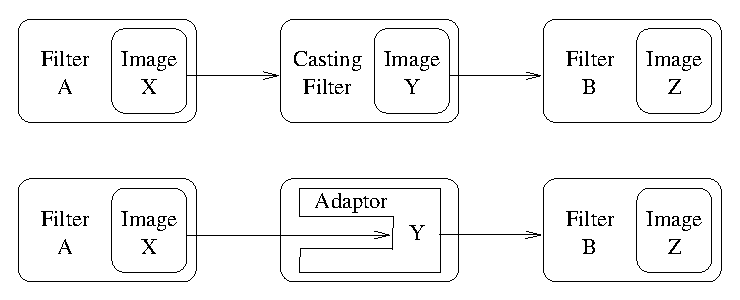
\includegraphics[width=0.8\textwidth]{ImageAdaptorConcept.eps}
\itkcaption[ImageAdaptor concept]{ The difference between using a
CastImageFilter and an ImageAdaptor.  ImageAdaptors
convert pixel values when they are accessed by iterators.  Thus, they do not
produces an intermediate image.  In the example
illustrated by this figure, the \emph{Image Y} is not created by the
ImageAdaptor; instead, the image is simulated on the fly each time an
iterator from the filter downstream attempts to access the image data.}
\label{fig:ImageAdaptorConcept}
\end{figure}

The purpose of an \emph{image adaptor} is to make one image appear
like another image, possibly of a different pixel type.  A typical
example is to take an image of pixel type \code{unsigned char} and
present it as an image of pixel type \code{float}. The motivation for
using image adaptors in this case is to avoid the extra memory
resources required by using a casting filter.  When we use the
\doxygen{CastImageFilter} for the conversion, the filter creates a
memory buffer large enough to store the \code{float} image. The
\code{float} image requires four times the memory of the
original image and contains no useful additional information. Image
adaptors, on the other hand, do not require the extra memory as
pixels are converted only when they are read using image iterators
(see Chapter~\ref{sec:ImageIteratorsChapter}).

Image adaptors are particularly useful when there is infrequent pixel access,
since the actual conversion occurs on the fly during the access operation. In
such cases the use of image adaptors may reduce overall computation time as
well as reduce memory usage. The use of image adaptors, however, can be
disadvantageous in some situations. For example, when the downstream filter
is executed multiple times, a CastImageFilter will cache its output after the
first execution and will not re-execute when the filter downstream is
updated. Conversely, an image adaptor will compute the cast every time.

Another application for image adaptors is to perform lightweight
pixel-wise operations replacing the need for a filter. In the toolkit,
adaptors are defined for many single valued and single parameter
functions such as trigonometric, exponential and logarithmic
functions. For example,
\begin{itemize}
\item \doxygen{ExpImageAdaptor}
\item \doxygen{SinImageAdaptor}
\item \doxygen{CosImageAdaptor}
\end{itemize}

The following examples illustrate common applications of image adaptors.

\section{Image Casting}
\label{sec:ImageAdaptorForBasicCasting}
\input{ImageAdaptor1.tex}


\section{Adapting RGB Images}
\label{sec:ImageAdaptorForRGB}
\input{ImageAdaptor2.tex}


\section{Adapting Vector Images}
\label{sec:ImageAdaptorForVectors}
\input{ImageAdaptor3.tex}


\section{Adaptors for Simple Computation}
\label{sec:ImageAdaptorForSimpleComputation}
\input{ImageAdaptor4.tex}


\section{Adaptors and Writers}

Image adaptors will not behave correctly when connected directly to a writer.
The reason is that writers tend to get direct access to the image buffer from
their input, since image adaptors do not have a real buffer their behavior in
this circumstances is incorrect. You should avoid instantiating the
\code{ImageFileWriter} or the \code{ImageSeriesWriter} over an image adaptor
type.

%%% \chapter{GUI}

Interface to GUI's such as FLTK, Qt, and wxWindows.

%%% \chapter{Wrapping.tex}

Using wrappers and generating wrappers


\chapter{Software Process}
\label{chapter:SoftwareProcess}

An outstanding feature of ITK is the software process used to develop,
maintain and test the toolkit. The Insight Toolkit software continues to
evolve rapidly due to the efforts of developers and users located around the
world, so the software process is essential to maintaining its quality. If
you are planning to contribute to ITK, or use the CVS source code repository,
you need to know something about this process (see
\ref{sec:ObtainingTheSoftware} on page \pageref{sec:ObtainingTheSoftware} to
learn more about obtaining ITK using CVS). This information will help you
know when and how to update and work with the software as it changes. The
following sections describe key elements of the process.

\section{CVS Source Code Repository}
\label{sec:CVSRepository}

\index{ITK!CVS repository}
\index{CVS}

The Concurrent Versions System (CVS) is a tool for version control
\cite{Fogel1999}. It is a very valuable resource for software projects
involving multiple developers.  The primary purpose of CVS is to keep
track of changes to software. CVS date and version stamps every
addition to files in the repository. Additionally, a user may set a
tag to mark a particular of the whole software. Thus, it is possible
to return to a particular state or point of time whenever desired. The
differences between any two points is represented by a ``diff'' file,
that is a compact, incremental representation of change. CVS supports
concurrent development so that two developers can edit the same file
at the same time, that are then (usually) merged together without
incident (and marked if there is a conflict). In addition, branches
off of the main development trunk provide parallel development of
software.

Developers and users can check out the software from the CVS repository. When
developers introduce changes in the system,  CVS facilitates to update the
local copies of other developers and users by downloading only the differences
between their local copy and the version on the repository.  This is an
important advantage for those who are interested in keeping up to date with the
leading edge of the toolkit. Bug fixes can be obtained in this way as soon as
they have been checked into the system.

ITK source code, data, and examples are maintained in a CVS repository.  The
principal advantage of a system like CVS is that it frees developers to try
new ideas and introduce changes without fear of losing a previous working
version of the software. It also provides a simple way to incrementally
update code as new features are added to the repository.



\section{DART Regression Testing System}
\label{sec:DART}
\label{sec:QualityDashboard}

\index{Dashboard}
\index{Quality Dashboard}
\index{Dart}

One of the unique features of the ITK software process is its use of the DART
regression testing system (\url{http://public.kitware.com/Dart}). In a
nutshell, what DART does is to provide quantifiable feedback to developers as
they check in new code and make changes. The feedback consists of the results
of a variety of tests, and the results are posted on a publicly-accessible
Web page (to which we refer as a \emph{dashboard}) as shown in
Figure~\ref{fig:Dashboard}. The most recent dashboard is accessible from
\url{http://www.itk.org/HTML/Testing.htm}). Since all users and developers of
ITK can view the Web page, the DART dashboard serves as a vehicle for
developer communication, especially when new additions to the software is
found to be faulty.  The dashboard should be consulted before considering
updating software via CVS.


\begin{figure}[ht]
\centering 
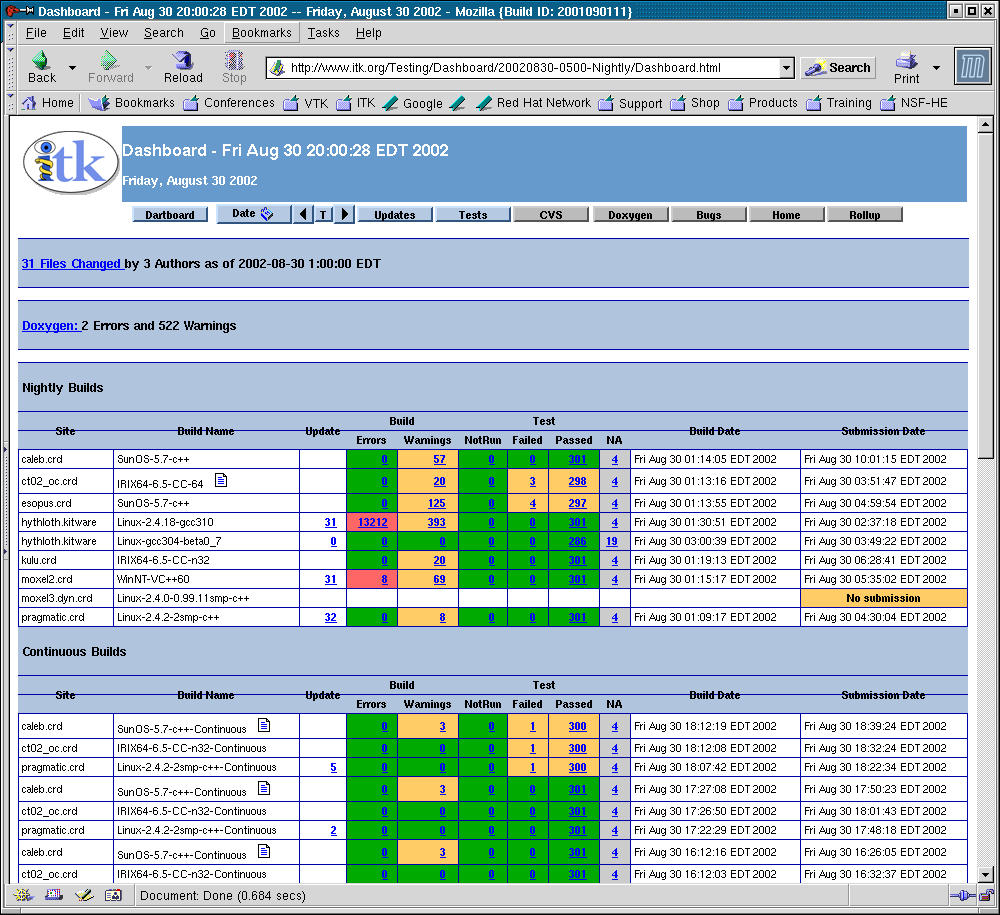
\includegraphics[width=0.7\textwidth]{Dashboard.eps}
\itkcaption[Dart Quality Dashboard]{On-line presentation of the quality
dashboard generated by DART.}
\label{fig:Dashboard}
\end{figure}

Note that DART is independent of ITK and can be used to manage quality
control for any software project. It is itself an open-source package and can
be obtained from

\begin{center} 
\url{http://public.kitware.com/Dart/HTML/Index.shtml}
\end{center} 

DART supports a variety of test types. These include the following.
\begin{description}
        \item[Compilation.] All source and test code is compiled and linked. 
        Any resulting errors and warnings are reported on the dashboard.

        \item[Regression.] Some ITK tests produce images as output. Testing
        requires comparing each test�s output against a valid baseline image. If
        the images match then the test passes. The comparison must be
        performed carefully since many 3D graphics systems (e.g., OpenGL)
        produce slightly different results on different platforms.

        \item[Memory.] Problems relating to memory such as leaks, uninitialized
        memory reads, and reads/ writes beyond allocated space can cause 
        unexpected results and program crashes. ITK checks run-time memory 
        access and management using Purify, a commercial package produced by 
        Rational. (Other memory checking programs will be added in the future.)

        \item[PrintSelf.] All classes in ITK are expected to print out all
        their instance variables (i.e., those with associated Set and Get 
        methods) correctly. This test checks to make sure
        that this is the case.

        \item[Unit.] Each class in ITK should have a corresponding unit test
        where the class functionalities are exercised and quantitatively
        compared against expected results. These tests are typically written
        by the class developer and should endeavor to cover all lines of code
        including \code{Set/Get} methods and error handling.

       \item[Coverage.] There is a saying among ITK developers: \emph{If it
        isn't covered, then it's broke.} What this means is that
        code that is not executed during testing is likely to be wrong. The
        coverage tests identify lines that are not executed in the
        Insight Toolkit test suite, reporting a total percentage
        covered at the end of the test. While it is nearly impossible to
        bring the coverage to 100\% because of error handling code and similar
        constructs that are rarely encountered in practice, the coverage
        numbers should be 75\% or higher. Code that is not covered well enough
        requires additional tests.
\end{description}

Figure~\ref{fig:Dashboard} shows the top-level dashboard web page. Each row
in the dashboard corresponds to a particular platform (hardware + operating
system + compiler). The data on the row indicates the number of compile
errors and warnings as well as the results of running hundreds of
small test programs. In this way the toolkit is tested both at compile time
and run time.

When a user or developer decides to update ITK source code from CVS it is
important to first verify that the current dashboard is in good shape. This
can be rapidly judged by the general coloration of the dashboard. A green
state means that the software is building correctly and it is a good day to
start with ITK or to get an upgrade. A red state, on the other hand, is an
indication of instability on the system and hence users should refrain from
checking out or upgrading the source code.

Another nice feature of DART is that it maintains a history of changes to the
source code (by coordinating with CVS) and summarizes the changes as part of
the dashboard. This is useful for tracking problems and keeping up to date
with new additions to ITK.

\section{Working The Process}
\label{sec:WorkingTheProcess}

The ITK software process functions across three cycles---the continuous
cycle, the daily cycle, and the release cycle.

The continuous cycle revolves around the actions of developers as they check
code into CVS. When changed or new code is checked into CVS, the DART
continuous testing process kicks in. A small number of tests are performed
(including compilation), and if something breaks, email is sent to all
developers who checked code in during the continuous cycle. Developers are
expected to fix the problem immediately.

The daily cycle occurs over a 24-hour period. Changes to the source base made
during the day are extensively tested by the nightly DART regression testing
sequence. These tests occur on different combinations of computers and
operating systems located around the world, and the results are posted every
day to the DART dashboard. Developers who checked in code are expected to
visit the dashboard and ensure their changes are acceptable---that is, they
do not introduce compilation errors or warnings, or break any other tests
including regression, memory, PrintSelf, and Set/Get. Again, developers are
expected to fix problems immediately.

The release cycle occurs a small number of times a year. This requires
tagging and branching the CVS repository, updating documentation, and
producing new release packages. Although additional testing is performed to
insure the consistency of the package, keeping the daily CVS build error free
minimizes the work required to cut a release.

ITK users typically work with releases, since they are the most
stable. Developers work with the CVS repository, or sometimes with periodic
release snapshots, in order to take advantage of newly-added features. It is
extremely important that developers watch the dashboard carefully, and
\emph{update their software only when the dashboard is in good condition
(i.e., is ``green'')}. Failure to do so can cause significant disruption if a
particular day's software release is unstable.

\section{The Effectiveness of the Process}
\label{sec:Effectiveness}

The effectiveness of this process is profound. By providing immediate
feedback to developers through email and Web pages (e.g., the dashboard), the
quality of ITK is exceptionally high, especially considering the complexity
of the algorithms and system. Errors, when accidently introduced, are caught
quickly, as compared to catching them at the point of release. To wait to the
point of release is to wait too long, since the causal relationship between a
code change or addition and a bug is lost. The process is so powerful that it
routinely catches errors in vendor's graphics drivers (e.g., OpenGL drivers)
or changes to external subsystems such as the VXL/VNL numerics library. All
of these tools that make up the process (CMake, CVS, and DART) are
open-source. Many large and small systems such as VTK (The Visualization
Toolkit \url{http://www.vtk.org}) use the same process with similar
results. We encourage the adoption of the process in your environment.


\fi

\backmatter


%%%%%%%%%%%%%%%%%%%%%%%%%%%%%%%%%%%%%%%%%
%
%  Insert the bibliography using BibTeX
%
%%%%%%%%%%%%%%%%%%%%%%%%%%%%%%%%%%%%%%%%%

\bibliographystyle{plain}
\bibliography{\bibtexdatabasepath}


%%%%%%%%%%%%%%%%%%%%%%%%%%%%%%%%%%%%%%%%%
%
%  Insert the Index file
%
%%%%%%%%%%%%%%%%%%%%%%%%%%%%%%%%%%%%%%%%%

\InputIfFileExists{SoftwareGuide.ind}


\end{document}



